\documentclass[12pt, a4paper, twoside]{article}
\usepackage[left=1in,right=1in,bottom=0.5in,top=0.8in]{geometry}
\usepackage{amsfonts}
\usepackage{amsmath, amssymb}
\usepackage{graphicx}
\usepackage[font=small,labelfont=bf]{caption}
\usepackage{epstopdf}
\usepackage[pdfpagelabels,hyperindex]{hyperref}
\usepackage{xcolor}
\usepackage{amsthm}
\usepackage{float}
\usepackage{pgfplots}
\usepackage{listings}
\usepackage{tikz-cd}
\usepackage{longtable}
\usepackage{mathrsfs}
\usepackage{mathtools}
\usepackage{hyperref}
\usepackage[most]{tcolorbox}
\usepackage{amssymb}
\usepackage{algorithm}
\usepackage{algpseudocode}
\usepackage{comment}
\usepackage{mathpartir}
\usepackage{braket}
\usepackage{tikz}
\usetikzlibrary{quantikz}
\usetikzlibrary{angles, quotes}
\pgfplotsset{compat=1.18}
\usepackage{soul}
\usepackage{xcolor}
\sethlcolor{yellow!40!white}
\usetikzlibrary{decorations.markings, arrows.meta}

\linespread{1.4}

\hypersetup{
pdftitle={.},
pdfauthor={Hojune Lee},
}

\newcommand{\overbar}[1]{\mkern 1.5mu\overline{\mkern-1.5mu#1\mkern-1.5mu}\mkern 1.5mu}
% newcommand bb
\newcommand{\BA}{{\mathbb {A}}} \newcommand{\BB}{{\mathbb {B}}}
\newcommand{\BC}{{\mathbb {C}}} \newcommand{\BD}{{\mathbb {D}}}
\newcommand{\BE}{{\mathbb {E}}} \newcommand{\BF}{{\mathbb {F}}}
\newcommand{\BG}{{\mathbb {G}}} \newcommand{\BH}{{\mathbb {H}}}
\newcommand{\BI}{{\mathbb {I}}} \newcommand{\BJ}{{\mathbb {J}}}
\newcommand{\BK}{{\mathbb {U}}} \newcommand{\BL}{{\mathbb {L}}}
\newcommand{\BM}{{\mathbb {M}}} \newcommand{\BN}{{\mathbb {N}}}
\newcommand{\BO}{{\mathbb {O}}} \newcommand{\BP}{{\mathbb {P}}}
\newcommand{\BQ}{{\mathbb {Q}}} \newcommand{\BR}{{\mathbb {R}}}
\newcommand{\BS}{{\mathbb {S}}} \newcommand{\BT}{{\mathbb {T}}}
\newcommand{\BU}{{\mathbb {U}}} \newcommand{\BV}{{\mathbb {V}}}
\newcommand{\BW}{{\mathbb {W}}} \newcommand{\BX}{{\mathbb {X}}}
\newcommand{\BY}{{\mathbb {Y}}} \newcommand{\BZ}{{\mathbb {Z}}}

% newcommand  scr
\newcommand{\sA}{{\mathscr {A}}} \newcommand{\sB}{{\mathscr {B}}}
\newcommand{\sC}{{\mathscr {C}}} \newcommand{\sD}{{\mathscr {D}}}
\newcommand{\sE}{{\mathscr {E}}} \newcommand{\sF}{{\mathscr {F}}}
\newcommand{\sG}{{\mathscr {G}}} \newcommand{\sH}{{\mathscr {H}}}
\newcommand{\sI}{{\mathscr {I}}} \newcommand{\sJ}{{\mathscr {J}}}
\newcommand{\sK}{{\mathscr {K}}} \newcommand{\sL}{{\mathscr {L}}}
\newcommand{\sN}{{\mathscr {N}}} \newcommand{\sM}{{\mathscr {M}}}
\newcommand{\sO}{{\mathscr {O}}} \newcommand{\sP}{{\mathscr {P}}}
\newcommand{\sQ}{{\mathscr {Q}}} \newcommand{\sR}{{\mathscr {R}}}
\newcommand{\sS}{{\mathscr {S}}} \newcommand{\sT}{{\mathscr {T}}}
\newcommand{\sU}{{\mathscr {U}}} \newcommand{\sV}{{\mathscr {V}}}
\newcommand{\sW}{{\mathscr {W}}} \newcommand{\sX}{{\mathscr {X}}}
\newcommand{\sY}{{\mathscr {Y}}} \newcommand{\sZ}{{\mathscr {Z}}}


% newcommand cal
\newcommand{\CA}{{\mathcal {A}}} \newcommand{\CB}{{\mathcal {B}}}
\newcommand{\CC}{{\mathcal {C}}} \newcommand{\CD}{{\mathcal {D}}}
\newcommand{\CE}{{\mathcal {E}}} \newcommand{\CF}{{\mathcal {F}}}
\newcommand{\CG}{{\mathcal {G}}} \newcommand{\CH}{{\mathcal {H}}}
\newcommand{\CI}{{\mathcal {I}}} \newcommand{\CJ}{{\mathcal {J}}}
\newcommand{\CK}{{\mathcal {K}}} \newcommand{\CL}{{\mathcal {L}}}
\newcommand{\CM}{{\mathcal {M}}} \newcommand{\CN}{{\mathcal {N}}}
\newcommand{\CO}{{\mathcal {O}}} \newcommand{\CP}{{\mathcal {P}}}
\newcommand{\CQ}{{\mathcal {Q}}} \newcommand{\CR}{{\mathcal {R}}}
\newcommand{\CS}{{\mathcal {S}}} \newcommand{\CT}{{\mathcal {T}}}
\newcommand{\CU}{{\mathcal {U}}} \newcommand{\CV}{{\mathcal {V}}}
\newcommand{\CW}{{\mathcal {W}}} \newcommand{\CX}{{\mathcal {X}}}
\newcommand{\CY}{{\mathcal {Y}}} \newcommand{\CZ}{{\mathcal {Z}}}

% newcommand frak
\newcommand{\fa}{{\mathfrak{a}}}  \newcommand{\fb}{{\mathfrak{b}}}
\newcommand{\fc}{{\mathfrak{c}}}  \newcommand{\fd}{{\mathfrak{d}}}
\newcommand{\fe}{{\mathfrak{e}}}  \newcommand{\ff}{{\mathfrak{f}}}
\newcommand{\fg}{{\mathfrak{g}}}  \newcommand{\fh}{{\mathfrak{h}}}
\newcommand{\fii}{{\mathfrak{i}}}  \newcommand{\fj}{{\mathfrak{j}}}
\newcommand{\fk}{{\mathfrak{m}}}  \newcommand{\fl}{{\mathfrak{l}}}
\newcommand{\fm}{{\mathfrak{m}}}  \newcommand{\fn}{{\mathfrak{n}}}
\newcommand{\fo}{{\mathfrak{o}}}  \newcommand{\fp}{{\mathfrak{p}}}
\newcommand{\fq}{{\mathfrak{q}}}  \newcommand{\fr}{{\mathfrak{r}}}
\newcommand{\fs}{{\mathfrak{s}}}  \newcommand{\ft}{{\mathfrak{t}}}
\newcommand{\fu}{{\mathfrak{u}}}  \newcommand{\fv}{{\mathfrak{v}}}
\newcommand{\fw}{{\mathfrak{w}}}  \newcommand{\fx}{{\mathfrak{x}}}
\newcommand{\fy}{{\mathfrak{y}}}  \newcommand{\fz}{{\mathfrak{z}}}

\newcommand{\fA}{{\mathfrak{A}}}  \newcommand{\fB}{{\mathfrak{B}}}
\newcommand{\fC}{{\mathfrak{C}}}  \newcommand{\fD}{{\mathfrak{D}}}
\newcommand{\fE}{{\mathfrak{E}}}  \newcommand{\fF}{{\mathfrak{F}}}
\newcommand{\fG}{{\mathfrak{G}}}  \newcommand{\fH}{{\mathfrak{H}}}
\newcommand{\fI}{{\mathfrak{I}}}  \newcommand{\fJ}{{\mathfrak{J}}}
\newcommand{\fK}{{\mathfrak{K}}}  \newcommand{\fL}{{\mathfrak{L}}}
\newcommand{\fM}{{\mathfrak{M}}}  \newcommand{\fN}{{\mathfrak{N}}}
\newcommand{\fO}{{\mathfrak{O}}}  \newcommand{\fP}{{\mathfrak{P}}}
\newcommand{\fQ}{{\mathfrak{Q}}}  \newcommand{\fR}{{\mathfrak{R}}}
\newcommand{\fS}{{\mathfrak{S}}}  \newcommand{\fT}{{\mathfrak{T}}}
\newcommand{\fU}{{\mathfrak{U}}}  \newcommand{\fV}{{\mathfrak{V}}}
\newcommand{\fW}{{\mathfrak{W}}}  \newcommand{\fX}{{\mathfrak{X}}}
\newcommand{\fY}{{\mathfrak{Y}}}  \newcommand{\fZ}{{\mathfrak{Z}}}



% newcommand :rm
\newcommand{\RA}{{\mathrm {A}}} \newcommand{\RB}{{\mathrm {B}}}
\newcommand{\RC}{{\mathrm {C}}} \newcommand{\RD}{{\mathrm {D}}}
\newcommand{\RE}{{\mathrm {E}}} \newcommand{\RF}{{\mathrm {F}}}
\newcommand{\RG}{{\mathrm {G}}} \newcommand{\RH}{{\mathrm {H}}}
\newcommand{\RI}{{\mathrm {I}}} \newcommand{\RJ}{{\mathrm {J}}}
\newcommand{\RK}{{\mathrm {K}}} \newcommand{\RL}{{\mathrm {L}}}
\newcommand{\RM}{{\mathrm {M}}} \newcommand{\RN}{{\mathrm {N}}}
\newcommand{\RO}{{\mathrm {O}}} \newcommand{\RP}{{\mathrm {P}}}
\newcommand{\RQ}{{\mathrm {Q}}} \newcommand{\RR}{{\mathrm {R}}}
\newcommand{\RS}{{\mathrm {S}}} \newcommand{\RT}{{\mathrm {T}}}
\newcommand{\RU}{{\mathrm {U}}} \newcommand{\RV}{{\mathrm {V}}}
\newcommand{\RW}{{\mathrm {W}}} \newcommand{\RX}{{\mathrm {X}}}
\newcommand{\RY}{{\mathrm {Y}}} \newcommand{\RZ}{{\mathrm {Z}}}

\newcommand{\Ad}{{\mathrm{Ad}}} \newcommand{\Aut}{{\mathrm{Aut}}}
\newcommand{\Br}{{\mathrm{Br}}} \newcommand{\Ch}{{\mathrm{Ch}}}
\newcommand{\cod}{{\mathrm{cod}}} \newcommand{\cont}{{\mathrm{cont}}}
\newcommand{\cl}{{\mathrm{cl}}}   \newcommand{\Cl}{{\mathrm{Cl}}}
\newcommand{\disc}{{\mathrm{disc}}}\newcommand{\Eis}{{\mathrm{Eis}}}
\newcommand{\Div}{{\mathrm{Div}}} \renewcommand{\div}{{\mathrm{div}}}
\newcommand{\End}{{\mathrm{End}}} \newcommand{\Frob}{{\mathrm{Frob}}}
\newcommand{\Gal}{{\mathrm{Gal}}} \newcommand{\GL}{{\mathrm{GL}}}
\newcommand{\Hom}{{\mathrm{Hom}}} \renewcommand{\Im}{{\mathrm{Im}}}
\newcommand{\Ind}{{\mathrm{Ind}}} \newcommand{\ind}{{\mathrm{ind}}}
\newcommand{\inv}{{\mathrm{inv}}}
\newcommand{\Isom}{{\mathrm{Isom}}} \newcommand{\Jac}{{\mathrm{Jac}}}
\newcommand{\ad}{{\mathrm{ad}}}  \newcommand{\Tr}{{\mathrm{Tr}}}
\newcommand{\Ker}{{\mathrm{Ker}}} \newcommand{\Ros}{{\mathrm{Ros}}}
\newcommand{\Lie}{{\mathrm{Lie}}} \newcommand{\Hol}{{\mathrm{Hol}}}

\newcommand{\cyc}{{\mathrm{cyc}}}\newcommand{\id}{{\mathrm{id}}}
\newcommand{\new}{{\mathrm{new}}} \newcommand{\NS}{{\mathrm{NS}}}
\newcommand{\ord}{{\mathrm{ord}}} \newcommand{\rank}{{\mathrm{rank}}}
\newcommand{\PGL}{{\mathrm{PGL}}} \newcommand{\Pic}{\mathrm{Pic}}
\newcommand{\cond}{\mathrm{cond}} \newcommand{\Is}{{\mathrm{Is}}}
\renewcommand{\Re}{{\mathrm{Re}}} \newcommand{\reg}{{\mathrm{reg}}}
\newcommand{\Res}{{\mathrm{Res}}} \newcommand{\Sel}{{\mathrm{Sel}}}
\newcommand{\RTr}{{\mathrm{Tr}}} \newcommand{\alg}{{\mathrm{alg}}}
\newcommand{\PSL}{{\mathrm{PSL}}}

\newcommand{\coker}{{\mathrm{coker}}}
\newcommand{\val}{{\mathrm{val}}} 
\newcommand{\sign}{{\mathrm{sign}}}
\newcommand{\mult}{{\mathrm{mult}}} 
\newcommand{\Vol}{{\mathrm{Vol}}}
\newcommand{\Meas}{{\mathrm{Meas}}}
\renewcommand{\mod}{\ \mathrm{mod}\ }
\newcommand{\Ann}{\mathrm{Ann}}
\newcommand{\Tor}{\mathrm{Tor}}
\newcommand{\Supp}{\mathrm{Supp}}
\newcommand{\supp}{\mathrm{supp}}
\newcommand{\Max}{\mathrm{Max}}
\newcommand{\Coker}{\mathrm{Coker}}
\newcommand{\Stab}{\mathrm{Stab}}
\newcommand{\Irr}{\mathrm{Irr}}
\newcommand{\Inf}{\mathrm{Inf}}
\newcommand{\Sup}{\mathrm{Sup}}
\newcommand{\rk}{\mathrm{rk}}
\newcommand{\Fil}{\mathrm{Fil}}
\newcommand{\Sim}{{\mathrm{Sim}}} 
\newcommand{\SL}{{\mathrm{SL}}}
\newcommand{\Spec}{{\mathrm{Spec}}} 
\newcommand{\SO}{{\mathrm{SO}}}
\newcommand{\SU}{{\mathrm{SU}}} 
\newcommand{\Sym}{{\mathrm{Sym}}}
\newcommand{\sgn}{{\mathrm{sgn}}} 
\newcommand{\tr}{{\mathrm{tr}}}
\newcommand{\tor}{{\mathrm{tor}}}  
\newcommand{\ur}{{\mathrm{ur}}}
\newcommand{\vol}{{\mathrm{vol}}}  
\newcommand{\ab}{{\mathrm{ab}}}
\newcommand{\Sh}{{\mathrm{Sh}}} 
\newcommand{\Ell}{{\mathrm{Ell}}}
\newcommand{\Char}{{\mathrm{Char}}}
\newcommand{\Tate}{{\mathrm{Tate}}}
\newcommand{\corank}{{\mathrm{corank}}} 
\newcommand{\Cond}{{\mathrm{Cond}}}
\newcommand{\Inn}{{\mathrm{Inn}}} 
\newcommand{\Spf}{{\mathrm{Spf}}}
\newcommand{\Mat}{{\mathrm{Mat}}}
\font\cyr=wncyr10  
\newcommand{\Sha}{\hbox{\cyr X}}
\newcommand{\wt}{\widetilde} 
\newcommand{\wh}{\widehat} 
\newcommand{\ck}{\check}
\newcommand{\pp}{\frac{\partial\bar\partial}{\pi i}}
\newcommand{\pair}[1]{\langle {#1} \rangle}
\newcommand{\wpair}[1]{\left\{{#1}\right\}}
\newcommand{\intn}[1]{\left( {#1} \right)}
\newcommand{\norm}[1]{\|{#1}\|}
\newcommand{\sfrac}[2]{\left( \frac {#1}{#2}\right)}
\newcommand{\ds}{\displaystyle}
\newcommand{\ov}{\overline}
\newcommand{\Gros}{Gr\"{o}ssencharaktere}
\newcommand{\incl}{\hookrightarrow}
\newcommand{\lra}{\longrightarrow}
\newcommand{\ra}{\rightarrow}
\newcommand{\imp}{\Longrightarrow}
\newcommand{\lto}{\longmapsto}
\newcommand{\bs}{\backslash}
\newcommand{\nequiv}{\equiv\hspace{-7.8pt}/}
\theoremstyle{plain}

\tcbuselibrary{theorems}

\tcbset{
    commonstyle/.style={
        enhanced,
        breakable,
        arc=2mm,
        fonttitle=\bfseries,
        description font=\normalfont,
        before skip=12pt,
        after skip=12pt,
        separator sign={.},
    }
}

\tcbset{thmstyle/.style={commonstyle, colback=blue!5, colframe=blue!30!black}}

\tcbset{defstyle/.style={commonstyle, colback=teal!5, colframe=teal!35!black}}

\tcbset{remstyle/.style={commonstyle, colback=orange!5, colframe=orange!40!black}}

\newtcbtheorem[number within=section]{thm}{Theorem}{thmstyle}{thm}
\newtcbtheorem[use counter from=thm]{cor}{Corollary}{thmstyle}{cor}
\newtcbtheorem[use counter from=thm]{prop}{Proposition}{thmstyle}{prop}
\newtcbtheorem[use counter from=thm]{lem}{Lemma}{thmstyle}{lem}
\newtcbtheorem[use counter from=thm]{conj}{Conjecture}{thmstyle}{conj}
\newtcbtheorem[use counter from=thm]{quest}{Question}{thmstyle}{quest}
\newtcbtheorem[use counter from=thm]{ppty}{Property}{thmstyle}{ppty}
\newtcbtheorem[use counter from=thm]{axiom}{Axiom}{thmstyle}{ax}
\newtcbtheorem[use counter from=thm]{claim}{Claim}{thmstyle}{clm}
\newtcbtheorem[use counter from=thm]{prob}{Problem}{thmstyle}{prob}

\newtcbtheorem[use counter from=thm]{defn}{Definition}{defstyle}{def}
\newtcbtheorem[use counter from=thm]{exmp}{Example}{defstyle}{ex}
\newtcbtheorem[use counter from=thm]{exer}{Exercise}{defstyle}{exe}
\newtcbtheorem[use counter from=thm]{notn}{Notation}{defstyle}{not}

\newtcbtheorem[use counter from=thm]{rem}{Remark}{remstyle}{rem}
\newtcbtheorem[use counter from=thm]{warn}{Warning}{remstyle}{wrn}

\author{Hojune Lee}

\title{Topology}
\begin{document}

\begin{titlepage}
    \begin{center}
        \vspace*{9cm}
            
        \Huge
        \textbf{Topology}
    
        \vspace{1cm}
        \large
        Summary with my Intuitions
        \vspace{3cm}
        
        \LARGE
        \textbf{Hojune Lee}
            
        \vspace{8cm}
            
        \normalsize
        \textbf{School of Computing, KAIST}\\  
    \end{center}
\end{titlepage}

\hypersetup{linkcolor=black}
\tableofcontents
\hypersetup{linkcolor=blue}

\newpage 

\section{Definition of Topology}

In many times, we \lq draw' some mathematical objects especially sets. One of the key intuition of studing topology is how can we \lq draw' such things. 
To draw somethings formally, we need to define bunch of things like \textit{shape of sets}. 
As we describe \textit{shape of groups} with its inner structures like subgroups, we describe \textit{shape of sets} with its inner structures like subsets. 

\begin{defn}{Topology}{defn_topology}
    A topology $\CT$ on a set $X$ is collection of subsets of $X$ having following axioms. 
    \begin{enumerate}
        \item $\emptyset, X \in \CT$
        \item $\CT$ is closed under arbitrary unions. 
        \item $\CT$ is closed under finite intersections. 
    \end{enumerate}
\end{defn}

Then \hl{we denote the pair $\intn{X, \CT}$ is \textit{topological space} (or just \textit{space}) and call every $U \in \CT$ by is \textit{open set} in $X$.} 
Then now $X$ is shaped by $\CT$ with certain axioms such that related subsets of $X$. This is very similar to defining groups. 

\begin{defn}{Group}{defn_group}
    Let $G$ be a set and $\star: G \times G \ra G$ is binary operation. $\intn{G, \star}$ is group when have following axioms. 
    \begin{enumerate}
        \item $\forall a, b, c \in G, \quad a \star (b \star c) = (a \star b) \star c$. 
        \item $\exists! 1_G \in G$ such that $\forall x \in G$, $1_G \star x = x \star 1_G = x$. 
        \item $\forall x \in G, \exists x^{-1} \in G$ such that $x \star x^{-1} = x^{-1} \star x = 1_G$. 
    \end{enumerate}
\end{defn}

Well, the definition of topology is quite less intuitive. However we already familiar with 
\lq shapes' in $\BR^n$ and often draw them in natural. Topology is just generalize such notions into general sets. 
In analysis in $\BR^n$, the key block was \textit{open balls}. We generalize this notion into general set also, which is called \textit{basis}. 

\begin{defn}{Basis}{defn_basis}
    A \textit{basis} $\CB$ is collection of subsets of $X$ having following axioms. 
    \begin{enumerate}
        \item $\forall x \in X$, $\exists B \in \CB$ such that $x \in B$. 
        \item $\forall B_1, B_2 \in \CB$, if $x \in B_1 \cap B_2$, $\exists B^* \in \CB$ such that $x \in B^* \subseteq B_1 \cap B_2$. 
    \end{enumerate}
\end{defn}

This is very natural property when we imagine open balls in $\BR^n$. Another good motivation to understand this is that, 
understand each $B \in \CB$ is collection of \lq near' elements. In metric space we'll define later, such notion of distance is very natural but here, 
we need to understand abstractically. This collection is called \textit{basis} since \hl{it generates some topology on $X$}.

\begin{defn}{Topology generated by Basis}{defn_topology generated by basis}
    Let $\CB$ is a basis of $X$. Then, define 
    \[\CT_\CB = \{U \subseteq X \mid \forall x \in U,~ \exists B \in \CB,~ x \in B \subseteq U\}\]
    Then $\CT_\CB$ is a topology on $X$ and called topology generated by $\CB$. 
\end{defn}

\begin{rem}{}{remark 1}
    $\CT_\CB$ is well-defined topology.
\end{rem}

As we noted $\CB$ \lq generates' some topology and it is called basis, there are more intuitive way to construct $\CT_\CB$. 

\begin{lem}{Topology generated by Basis}{lem_topology generated by basis}
    $\CT_\CB = $ collection of all unions in $\CB$.  
\end{lem}

Then next the natural question is that, \textit{can we compare 2 topologies with its basis}? 
The answer is yes, and we'll use following theorem in many times. Following theorem allows us to 
compare the inclusion relation (or equivalence relation) of 2 topologies via its basis. 

\begin{thm}{Topology Comparison with Basis}{thm_topology comparison with basis}
    Let $\CB_1, \CB_2$ be basis of $X$ and $\CT_1, \CT_2$ be topology of $X$ generated by $\CB_1, \CB_2$ respectively. 
    Then $\CT_1 \subseteq \CT_2$ if and only if $\forall x \in X$, $\forall B_1 \in \CB_1$ such that $x \in B_1$, there exists $B_2 \in \CB_2$ such that $x \in B_2 \subseteq B_1$. 
\end{thm}

We observe that once we have basis $\CB$, then we can generate some topology by unioning them. 
However, in \ref{def:defn_topology} topology is closed under not only union but also finite intersection. 
So we can define more light basis for topology(or, basis for basis). 

\begin{defn}{Subbasis}{defn_subbasis}
    A subbasis $\CS$ is collection of subsets of $X$ having following axiom. 
    \begin{enumerate}
        \item $\forall x \in X$, $\exists S \in \CS$ such that $x \in S$. 
    \end{enumerate}
    equivalently, the entire union of $\CS$ is $X$. 
\end{defn}

Then, we can observe that 
\[\CS \xrightarrow{\text{finite intersections}} \CB \xrightarrow{\text{arbitrary unions}} \CT\]

\newpage 

\section{Some Basic Famous Topologies}

In this section, we'll define a few useful topologies. 

\begin{defn}{Standard Topology}{defn_standard topology}
    Let $X = \BR$ and $\CB = \{(a, b) \mid a < b\}$. $\CT_\CB$ is called standard topology of $\BR$. 
\end{defn}

\begin{defn}{Lower Limit Topology}{defn_lower limit topology}
    Let $X = \BR$ and $\CB = \{[a, b) \mid a < b\}$. $\CT_\CB$ is called lower limit topology of $\BR$. 
\end{defn}

\begin{defn}{Order Topology}{defn_order topology}
    Let $X$ be a simply ordered set. i.e., $\forall x, y \in X$, $x < y$ or $x = y$ or $y < x$ holds and the relation $<$ is transitive.
    Then we define standard topology for $X$ which is called order topology. Let 
    \[\CB = \begin{cases}
        (a, b) & \forall a < b \in X \\
        [m, b) & m \text{ is smallest element in }X \\
        (a, M] & M \text{ is largest element in }X 
    \end{cases}\]
    Topology generated by this $\CB$ on simply ordered set $X$ is called \textit{order topology}. 
\end{defn}

For order topology, we can define subbasis generates such basis. It is called open rays and define by 
\[\CS = \{(-\infty, a), (a, \infty) \mid a \in X\}\]
\begin{rem}{}{rem_2.4}
    $\CS$ is subbasis of $\CB$. 
\end{rem}

One obvious step is defining \lq sub' space and find its natural topology. The most natural 
definition is that, if $Y$ is subspace of $X$, it inherits all open sets in $X$ into $Y$. means that, 
\[\textit{If $Y$ is subspace of $X$, then open sets in $X$ is also open in $Y$.}\]

\vspace{1mm}

\begin{defn}{Subspace Topology}{defn_subspace topology}
    Let $(X, \CT_X)$ is a topological space and $Y \subseteq X$. We define 
    \[\CT_Y = \{U \cap Y \mid U \in \CT_X\}\]
    for topology of $Y$ and call \textit{subspace topology}. And $(Y, \CT_Y)$ is called \textit{subspace} of $X$. 
\end{defn}

Then similarly the basis of $\CT_Y$ has same relation. 
\[\textit{$\CB_Y = \{B \cap Y \mid B \in \CB_X\}$ is basis for $\CT_Y$.}\]

\begin{warn}{}{warn_2.6}
    Open sets in general $Y \subseteq X$ do not need to also open in $X$. 
\end{warn}

\begin{lem}{When open sets in $Y$ is also open in $X$?}{lem_2.7}
    If $Y$ is subspace of $X$ and $Y$ is open in $X$, then open sets in $Y$ is also open in $X$.
\end{lem}

\begin{proof}
    From definition, any open set $V \in \CT_Y$ in $Y$ is formed $V = U \cap Y$ and $U, Y \in \CT_X$ so $V \in \CT_X$.
\end{proof}

Then also one natural question is arised. \hl{How about subspace of simply ordered space?}
Here interesting results are occur. We observe 3 subspace of $\BR$. 
\[Y_1 = [0, 1], \quad Y_2 = [0, 1) \cup \{2\}, \quad Y_3 = [0, 1] \cup [2, 3]\]
In $Y_1, Y_3$, subspace topology of them are equivalent to ordered topology of themselves. 
However, in $Y_2$, subspace topology is not equivalent to ordered topology since then singleton set $\{2\}$ is open in 
subspace topology but not in ordered topology. In general, 
\begin{thm}{Subspace Topology and Order Topology}{thm_subspace topology and ordered topology}
    Let $(X, \CT_X)$ is ordered topology space and $Y \subseteq X$. $\CT_1$ is subspace topology of $Y$ and $\CT_2$ is ordered topology of $Y$. (since $Y$ also simply ordered)
    Then, $\CT_2 \subseteq \CT_1$ in general. Furthermore, $\CT_1 = \CT_2$ if and only if every gap in $Y$ is either open or closed. 
\end{thm}

\newpage 

\section{Closed Sets and Limit Points}

We defined basic notions of topology via well-shaped subsets called \textit{open sets}. 
Another type of sets can be useful. 

\begin{defn}{Closed Sets}{defn_closed sets}
    $C \subset X$ is closed when $X \setminus C$ is open in $X$ 
\end{defn}

Openess and closedness is familiar notion in $\BR^n$ space. Closed set is generalization of the closedness into general sets. 
Sometimes, arguing with closed set is much easier than open sets despite they are just complement of open sets. 

\begin{thm}{Topology Axioms for Closed Sets}{thm_3.2}
    Let $(X, \CT)$ be a topological space. Then following variation of axioms hold. 
    \begin{enumerate}
        \item $\emptyset, X$ is closed set. 
        \item Arbitrary intersections of closed sets are closed. 
        \item Finite unions of closed sets are closed. 
    \end{enumerate}
\end{thm}

\begin{thm}{Subspace Topology for Closed Sets}{thm_3.3}
    Let $Y$ be subspace of $X$. Then, $D \subseteq Y$ is closed in $Y$ if and only if 
    there exists closed set $C$ in $X$ such that $D = C \cap Y$. 
\end{thm}

\begin{proof}
    If $D \subseteq Y$ is closed, then $Y \setminus D$ is open in $Y$. So, we can find 
    open set $U$ in $X$ such that $Y \setminus D = U \cap Y$. Then, $D = U^c \cap Y$ and $U^c$ is closed in $X$. If $D = C \cap Y$ for closed set $C$ in $X$, 
    $Y \setminus D = Y \cap C^c$ is open in $Y$, so $D$ is closed in $Y$. 
\end{proof}

\begin{thm}{When closed sets in $Y$ is also closed in $X$?}{thm_3.4}
    If $Y$ is subspace of $X$ and $Y$ is closed in $X$, then closed sets in $Y$ is closed in $X$. 
\end{thm}

Now we define few more way to construct meaningful sets. 

\begin{defn}{Interior and Closure of a Set}{defn_interior and closure}
    Let $A$ be any subset of $X$. The interior of $A$ (denoted by $\text{Int } A$) is union of all open sets contained in $A$. i.e., 
    the largest open set in $A$. The closure of $A$ (denoted by $\overbar{A}$) is intersection of all closed sets containing $A$. i.e., 
    the smallest closed set containing $A$. 
\end{defn}

In many times, closure of set acts quite important roles. So we state few theorems related to the closure of set. 

\begin{thm}{Closure in the Subspace}{thm_3.6}
    Let $X$ be a topological space and $Y$ is subspace of $X$. 
    For $A \subseteq Y \subseteq X$, denote $\overbar{A}$ by closure of $A$ in $X$. Then closure of $A$ in $Y$ is 
    determined by $\overbar{A} \cap Y$. 
\end{thm}

\begin{proof}
    Let $C$ be closed set in $X$ such that $A \subseteq C$. 
    Then, $C \cap Y$ is closed in $Y$ and $A \subseteq C \cap Y$. 
    So, $\overbar{A} \cap Y \subseteq$ closure of $A$ in $Y$. 
    And for $D$ be closed set in $Y$ such that $A \subseteq D$, 
    by definition, $D = C \cap Y$ where $C$ is closed and $A \subseteq C$. 
    So, closure of $A$ in $Y$ is equivalent to $\overbar{A} \cap Y$. 
\end{proof}

\begin{thm}{Points in Closure}{thm_points in closure}
    Let $X$ be a topological space and $A \subseteq X$ be any subset. 
    Then $x \in \overbar{A}$ if and only if every \textit{neighborhoods} of $x$ \textit{intersects} with $A$.
\end{thm}

Here, \textit{neighborhood} of $x$ means that any open sets containing $x$. Also, we say $A, B$ are intersects when $A \cap B \neq \emptyset$. 
This is important property of points in the closure. 

\begin{proof}
    If $x \in \overbar{A}$ but $\exists \, U$ which is neighborhood of $x$ and $U \cap A = \emptyset$, 
    Then $A \subseteq U^c$ and $U^c$ is closed. So by definition, $\overbar{A} \subseteq U^c$ so $x \in U^c$ which is contradiction. 
    If every neighborhoods of $x$ intersects with $A$ but $x \notin \overbar{A}$, 
    then it means that there exists a closed set $C$ such that containing $A$ but does not contain $x$.
    It implies that $x \in X \setminus C$ and $X \setminus C \cap A = \emptyset$ which is contradiction. 
\end{proof}

\begin{defn}{Limit Points}{defn_limit points}
    If $A$ is a subset of topological space $X$, we say that $x$ is a limit point of $A$ when 
    every neighborhoods of $x$ intersects with $A$ other than $x$ itself. i.e., $x \in \overbar{A \setminus \{x\}}$. 
\end{defn}

Then now, \hl{we can describe the closure of set $A$ with $A$ itself and its limit points.}

\begin{thm}{Closure Representation}{thm_closure representation}
    Let $X$ be a topological space and $A \subseteq X$ be any subset. 
    Denote $A'$ by set of limit points of $A$. Then, 
    \[\overbar{A} = A \cup A'\]
    In other words, $\overbar{A} \setminus A = $ limit points of $A$ but not in $A$.
\end{thm}

\begin{cor}{When $A$ is closed?}{cor_3.10}
    $A \subseteq X$ is closed if and only if $A' \subseteq A$. i.e., $A$ contains all of its limit points. 
\end{cor}

\newpage 

\section{Basic notion of Hausdorff Space}

We learned how can we define each shapes of sets and construct them into spaces. 
\hl{Then we can wonder, what is the good shapes for spaces? And how can we categorize them?}
Actually the answer for this question is dealt in further section but we define very part of them here
since it will be heavily used. 

\begin{defn}{Hausdorff Space}{defn_Hausdorff space}
    A topological space $(X, \CT)$ is called Hausdorff space when 
    \[\textit{$\forall \, x \neq y \in X$, there exists disjoint neighborhoods of $x, y$ respectively.}\]
    In other words, we can \textit{seperate} two \textit{points} via their neighborhoods always. 
\end{defn}

Actually we can understand that why this is good property for space since real line $\BR$ 
have this property. Once our space is Hausdorff, we can find a few interesting facts. 

\begin{thm}{Finite sets in Hausdorff spaces}{thm_4.2}
    Let $X$ be a Hausdorff space. Then, every finite set in $X$ is closed. 
\end{thm}

\begin{proof}
    Since finite union of closed sets are closed, so it is sufficient to show that 
    any singleton set $\{x\}$ is closed in $X$. Now suppose that $y \in X$ is a limit point of $\{x\}$. 
    If $x \neq y$, since $X$ is Hausdorff we can find $U_1, U_2$ such that both are neighborhoods of $x, y$ respectively and $U_1 \cap U_2 = \emptyset$. 
    Then, according to theorem \ref{thm:thm_points in closure},  $y$ can't be limit point of $\{x\}$. 
    So unless $x$ is limit point or not, we can state $\{x\}$ contained all its limit points and so closed set. 
\end{proof}

Now we find next interesting property of Hausdorff space. Let's call the $\BN$-indexed sets of points in $X$ by \textit{sequences} and denoted by $\{x_n\}_{n \in \BN}$. 
In general notion, we state that $\{x_n\}_{n \in \BN}$ converges to $x \in X$ when 
\[\textit{For any neighborhood $U$ of $x$, we can find $N \in \BN$ such that $x_m \in U$ for $m \geq N$.}\]
Then following good property holds in Hausdorff space. 

\begin{thm}{Unique Convergency in Hausdorff Space}{thm_unique convergency in Hausdorff space}
    If $X$ is a Hausdorff space, then any sequences in $X$ converges into at most one point.
\end{thm}

\begin{thm}{Hausdorff spaces with Famous Topologies}{thm_4.4}
    Any space with Order topology, Subspace topology of Hausdorff space is Hausdorff. 
\end{thm}

\newpage 

\section{Continuous Functions and Homeomorphisms}

From highschool to undergrad analysis courses, the continuity of function is matter. 
By the way, the concept of continuity in $\BR^n$(in general, metric space) is quite obvious.
Our goal is generalize them into general topological space. One beautiful definition is following. 

\begin{defn}{Continuous Function}{defn_continuous function}
    Let $X, Y$ be any topological spaces. A function $f: X \rightarrow Y$ is \textit{continuous} 
    when for any open set $V$ in $Y$, the preimage $f^{-1}(V) \subseteq X$ is also open set in $X$. 
\end{defn}

\begin{rem}{}{rem_5.2}
    Continuity is depends on not only $f$ itself but also topologies of $X$ and $Y$. 
\end{rem}

Here, I mention why we take preimage for define continuity. First at all, this notion is called 
\hl{pull-back}. This is important since it preserves many structural things in codomain space $Y$. 

\begin{prop}{Preimage Propositions}{prop_5.3}
\begin{enumerate}
    \item $f^{-1}(A \cap B) = f^{-1}(A) \cap f^{-1}(B)$
    \item $f^{-1}(A \cup B) = f^{-1}(A) \cup f^{-1}(B) $
    \item $f^{-1}(A^c) = \left(f^{-1}(A)\right)^c$
\end{enumerate}
\end{prop}

These are not true in original mapping $f$. So, we can analyze topological structures of $Y$ in $X$ via pull-back. 
Also, the natural notion $\varepsilon$-$\delta$ definition of continuity also refer the preimage. 
Once we view this definition as just generalization of $\varepsilon$-$\delta$ definition, it seemed be natural. 

\begin{lem}{Checking Continuity}{lem_5.4}
    Let $\CS$ be subbasis of topological space $Y$. Then for any $S \in \CS$, if $f^{-1}(S)$ is open set in $X$, $f$ is continuous. 
\end{lem}

\begin{proof}
    Every open sets in $Y$ can be generated by arbitrary union and finite intersection of elements in $\CS$. 
    Since \ref{prop:prop_5.3} holds for preimages, if every $f^{-1}(S)$ is open then every preimage of open set is also open in $X$. 
\end{proof}

\newpage 

\begin{thm}{Equivalence statements for Continuity}{thm_5.5}
    The followings are equivalent. 
    \begin{enumerate}
        \item $f$ is continuous.
        \item For any $A \subset X$, $f(\overbar{A}) \subseteq \overbar{f(A)}$
        \item For every closed set $C$ of $Y$, $f^{-1}(C)$ is closed in $X$. 
        \item For each $x \in X$, each neighborhood $V$ of $f(x)$, there exists neighborhood $U$ of $x$ such that $f(U) \subseteq V$. 
    \end{enumerate}
\end{thm}
(4) is just changing of forms of statement into $\varepsilon$-$\delta$ definition form. 
The remarkable one is second one. It can be written: \hl{If $x$ is a limit point of $A$ in $X$, then $f(x)$ is a limit point of $f(A)$ in $Y$} or equivalently, 
\hl{continuous map preserves the limit point relation}. 

\begin{defn}{Homeomorphism}{defn_homeomorphism}
    Let $X, Y$ be topological spaces and $f: X \rightarrow Y$ is a bijection. If both $f, f^{-1}$ are continuous 
    then $f$ is called \textit{homeomorphism} and $X, Y$ are \textit{homeomorphic}. 
\end{defn}

The homeomorphism $f$ between $X$ and $Y$ construct bijection between $\CT_X$ and $\CT_Y$ also. i.e., open sets in both spaces are one-to-one corresponds. 
We say that \hl{some property is topological property if it preserves by homeomorphisms}. 
And also we say that an injective continuous map $f: X \rightarrow Y$ is \textit{embedding}. 

\begin{thm}{Constructing Continuous Functions}{thm_constructing continuous functions}
Let $X, Y$ and $Z$ be topological spaces. 
\begin{enumerate}
    \item Any constant function is continuous. 
    \item If $A$ is a subspace of $X$, the natural inclusion $j: A \hookrightarrow X$ is continuous. 
    \item If $f: X \rightarrow Y$ and $g: Y \rightarrow Z$ are continuous, then $h = g \circ f$ is continuous. 
    \item If $f: X \rightarrow Y$ is continuous then for subspace $A$ of $X$, $f|_A : A \rightarrow Y$ is continuous. 
    \item Let $f: X \rightarrow Y$ is continuous. If $\Im(X)$ is subspace of $Y$, then $g: X \rightarrow \Im(X)$ is continuous. If $Y$ is subspace of $Z$, then $h: X \rightarrow Z$ is continuous. 
    \item If $X = \bigcup U_\alpha$ and every $f|_{U_\alpha}$ is continuous, then $f: X \rightarrow Y$ is continuous.
\end{enumerate}
\end{thm}

These are not hard to follow and prove. We state important lemma here. 

\begin{lem}{Pasting Lemma}{lem_pasting lemma}
    Let $X, Y$ be topological spaces and $X = A \cup B$ where \hl{$A, B$ are closed subspaces in $X$.} 
    Let $f: A \rightarrow Y$ and $g: B \rightarrow Y$ be continuous. If $f(x) = g(x)$ for every $x \in A \cap B$, 
    then we can define continuous function $h: X \rightarrow Y$ defined by 
    \[h(x) = \begin{cases}
        f(x) & x \in A \\
        g(x) & x \in B   
    \end{cases}\]
    This is well-defined since we assume $f(x) = g(x)$ for $x \in A \cap B$. 
\end{lem}

\begin{proof}
    As we stated, $h: X \rightarrow Y$ is well-defined. Let $C$ be any closed set in $Y$. Then, $f^{-1}(C), g^{-1}(C)$ are closed in $A, B$ respectively by \ref{thm:thm_5.5}. 
    However since $A, B$ are closed subspace of $X$, $f^{-1}(C), g^{-1}(C)$ is closed in $X$ by \ref{thm:thm_3.4}. 
    However, 
    \[h^{-1}(C) = f^{-1}(C) \cup g^{-1}(C) \implies \text{ closed in $X$ }\]
    So, $h: X \rightarrow Y$ is continuous function. 
\end{proof}

\newpage 

\section{The Product Topology}

We often consider Cartesian product of sets(or spaces). It is good time to state how Cartesian product can be generalized into topological concepts. 
We'll see familiar product $X \times Y$ first and than generalize into arbitrary Cartesian product $\prod_{\alpha \in J} X_\alpha$ for indice set $J$. 

\begin{defn}{Simple Cartesian Product Space $X \times Y$}{defn_simple cartesian product}
    Let $(X, \CT_X), (Y, \CT_Y)$ be a topological spaces. For the Cartesian product $X \times Y$, 
    we define \textit{product topology} generated by following basis. 
    \[\CB := \{U \times V \mid U \in \CT_X, \, V \in \CT_Y\}\]
\end{defn}

\begin{rem}{}{rem_6.2}
    We take $\CT_X \times \CT_Y$ as just a \textcolor{red}{basis} for $X \times Y$. 
    So, the \textit{product topology} on $X \times Y$ is arbitrary unions of $\CT_X \times \CT_Y$. 
    Intuitively, imagine the $\BR^2 = \BR \times \BR$ space. 
    The \lq shapes' in $\BR^2$ is more various than just $\CT_\BR \times \CT_\BR$. So, $\CT_X \times \CT_Y$ just basis generates product topology. 
\end{rem}

Here we can check a few properties that we stated in previous sections. 

\begin{lem}{Basis of Product Topology}{lem_basis of product topology}
    Let $X, Y$ be topological spaces. If $\CB_X, \CB_Y$ are basis for $X, Y$ respectively, 
    then $\CB = \CB_X \times \CB_Y$ is a basis for product topology of $X \times Y$. 
\end{lem}

\begin{defn}{Projection}{defn_projection}
    We define $\pi_1: X \times Y \rightarrow X$ and $\pi_2: X \times Y \rightarrow Y$ in natural manner. 
\end{defn}

\begin{lem}{Subbasis of Product Topology}{lem_subbasis of product topology}
    Let $X, Y$ be topological spaces. Following is subbasis for product topology of $X \times Y$: 
    \[\CS = \{\pi_1^{-1}(U) \mid U \text{ is open in $X$}\} \cup \{\pi_2^{-1}(V) \mid Y \text{ is open in $Y$}\}\]
\end{lem}

\begin{lem}{Subspace of Product Space}{lem_subspace of product space}
    Let $X, Y$ be topological spaces. If $A, B$ are subspaces of $X, Y$ respectively, then 
    $A \times B$ is subspace of $X \times Y$. 
\end{lem}

\begin{lem}{Product of Hausdorff is Hausdorff}{lem_product of Hausdorff is Hausdorff}
    If $X, Y$ are Hausdorff space, then $X \times Y$ with product topology is Hausdorff. 
\end{lem}

These are not hard to understand. We can easily generalize this into finite Cartesian product by 
\[X_1 \times X_2 \times \cdots \times X_n\]

Then here \ref{lem:lem_subbasis of product topology} still holds. One natural following step is considering the arbitrary 
Cartesian products. 

\begin{defn}{Indexing, $J$-tuple and Coordinates}{defn_indexing, J-tuple and coordinates}
    Let $J$ be an arbitrary index set. Given a set $X$, we define a $J$-tuple of elements of $X$ to be a function 
    \[\mathbf{x}: J \rightarrow X\]
    We often denote $\mathbf{x}(\alpha)$ by $x_\alpha$ and call it the $\alpha$-th coordinate of $\mathbf{x}$. 
\end{defn}

With this arbitrary index set $J$, we can define general Cartesian product. 

\begin{defn}{Cartesian Product}{Cartesian product}
    Let $J$ be an arbitrary index set and $\{A_\alpha\}_{\alpha \in J}$ be an indexed family of sets.
    The Cartesian product of this indexed family is denoted by 
    \[\prod_{\alpha \in J}A_\alpha = \{\text{All $J$-tuples $\{x_\alpha\}_{\alpha \in J}$ \, where each $x_\alpha \in A_\alpha$}\}\]
\end{defn}

Now we can define this notion into topological Cartesian product space. However, there are 2 ways to construct topology on such space. 
Actually, \hl{one is quite natural but less useful, and the other is related to $\ref{lem:lem_subbasis of product topology}$. It means that $\ref{lem:lem_subbasis of product topology}$ is not the case in general, 
and two topologies are distinct when $J$ is an infinite index set}. 

\begin{defn}{Box Topology}{Box topology}
    Given arbitrary index set $J$ and $\{X_\alpha\}_{\alpha \in J}$ be a family of topological spaces. 
    Then, we can find Cartesian product $\prod_{\alpha \in J}X_\alpha$. Then we can define a basis in following way: 
    \[\CB = \left\{\prod_{\alpha \in J} U_\alpha \mid U_\alpha \text{ is open in $X_\alpha$}\right\}\]
    Then this is topology on $\prod_{\alpha \in J} X_\alpha$ and called \textit{box topology}. 
\end{defn}

\newpage 

\begin{defn}{Projection}{projection}
    For each $\beta \in J$, we define 
    \[\pi_\beta: \prod_{\alpha \in J} X_\alpha \rightarrow X_\beta\]
    defined by 
    \[\pi_\beta: \mathbf{x} \mapsto \mathbf{x}(\beta)\]
    This is called the projection mapping associated with the index $\beta$. 
\end{defn}

We generalize the notion of projection in \ref{def:defn_projection} into general Cartesian product. 

\begin{defn}{Product Topology}{product topology}
    We can define a subbasis $\CS$ of $\prod_{\alpha \in J} X_\alpha$ in following way: 
    \[\CS_\beta = \left\{\pi_\beta^{-1}(U_\beta) \mid U_\beta \text{ is open in } X_\beta \right\} \implies \CS = \bigcup_{\beta \in J} \CS_\beta\]
    The topology generated by this subbasis is called the \textit{product topology}. 
    And with this, $\prod_{\alpha \in J} X_\alpha$ is called \textit{product space}. 
\end{defn}

Compare these two topology is not quite difficult. 
As we stated in \ref{thm:thm_topology comparison with basis}, it is enough to show the differences between 
the basis of box topology and the basis of product topology. 

\begin{prop}{Comparison between Box topology and Product Topology}{box topology versus product topology}
    The basis of box topology contains all possible forms of $\prod_{\alpha \in J} U_\alpha$ where $U_\alpha$ is any open set in $X_\alpha$. 
    However, the basis of product topology is obtained by \textcolor{red}{finite intersections} of subbasis. 
    So, the basis of product topology contains only has the following form of elements: 
    \[\pi_{\beta_1}^{-1}(U_{\beta_1}) \cap \cdots \cap \pi_{\beta_n}^{-1}(U_{\beta_n}) = \prod_{\alpha \in J} U_\alpha, \quad U_\alpha = \begin{cases}
        X_\alpha & \alpha \notin \{\beta_1, \cdots, \beta_n\} \\
        U_{\beta_i} & i \in [n]
    \end{cases} \]
    So the basis of box topology contains the basis of product topology, so \textit{box topology is finer than product topology}. 
\end{prop}

According to the textbook \cite{munkres}, there is an answer \hl{why we generally use the definition of product topology}. 
i.e., despite the definition of box topology is more finer and stronger, we assume that the topology of $\prod_{\alpha \in J}X_\alpha$ will be 
product topology in general. It is because, there are many important theorems in topology 
such that holds for product topology, but fails for box topology. 
\hl{However note that when index set $J$ is infinite then matter. For finite Cartesian product of spaces, there are not any confusion.}

Now let's state bunch of theorems here. 

\begin{thm}{Basis generated by Basis of each Space}{6.14}
    Suppose that $\{X_\alpha\}_{\alpha \in J}$ be family of spaces and $\CB_\alpha$ is the basis of $X_\alpha$. 
    Then, the basis of \textit{box topology} is given by 
    \[\CB_{\text{box}} = \left\{\prod_{\alpha \in J}B_\alpha \mid B_\alpha \in \CB_\alpha\right\}\]
    The basis of \textit{product topology} is given by 
    \[\CB_{\text{prod}} = \left\{\prod_{\alpha \in J} B_\alpha \mid B_\alpha = \begin{cases}
    B_\alpha \in \CB_\alpha & \text{Finitely many $\alpha$} \\
    X_\alpha & \text{otherwise}
    \end{cases}\right\}\]
\end{thm}

\begin{thm}{Subspace Topology and Box and Product Topology}{6.15}
    Let $A_\alpha$ be a subspace of $X_\alpha$ for each $\alpha \in J$. 
    Now box topology of $\prod_{\alpha \in J} A_\alpha$ is subspace of box topology of $\prod_{\alpha \in J} X_\alpha$. 
    And same for product topology. 
\end{thm}

\begin{thm}{Hausdorff in Box and Product Topology}{6.16}
    If each $X_\alpha$ is Hausdorff, $\prod{\alpha \in J} X_\alpha$ is also Hausdorff in both box and product topologies. 
\end{thm}

\begin{thm}{Closure in Box and Product Topology}{6.17}
    Let $A_\alpha \subseteq X_\alpha$ for each $\alpha \in J$. If $\prod X_\alpha$ is given either the product or the box topology, then 
    \[\prod \overbar{A_\alpha} = \overbar{\prod A_\alpha}\]
\end{thm}

\begin{proof}

Suppose that $\mathbf{x} = (x_\alpha)_{\alpha \in J} \in \prod \overbar{A_\alpha}$. 
Then, let $\prod U_\alpha$ be any basis neighborhood of $\mathbf{x}$ in box or product topology of $\prod X_\alpha$. 
Then each $U_\alpha$ is neighborhood of $x_\alpha$ in $X_\alpha$, and since $x_\alpha \in \overbar{A_\alpha}$ so we can find 
$y_\alpha \in A_\alpha \cap U_\alpha$. So, $\mathbf{y} = (y_\alpha)_{\alpha \in J} \in \prod U_\alpha \cap \prod A_\alpha$. So $\mathbf{x} \in \overbar{\prod{A_\alpha}}$. 

Suppose that $\mathbf{x} \in \overbar{\prod A_\alpha}$. 
Let $V_\beta$ be an arbitrary open set of $X_\beta$ containing $x_\beta$. Since $\pi^{-1}_\beta(V_\beta)$ is open in $\prod A_\alpha$ in both topology and containing $\mathbf{x}$, 
there exists $\mathbf{y} \in \pi_\beta^{-1}(V_\beta) \cap \prod A_\alpha$. 
This implies that, $y_\beta \in V_\beta \cap A_\beta$. So, $x_\beta \in \overbar{A_\beta}$. 
\end{proof}

\newpage 
\hl{Following is the first situation when we can observe box topology and product topology is different.}
\begin{thm}{Continuity in Product Topology}{6.18}
    Let $f: A \rightarrow \prod X_\alpha$ be given by the equation 
    \[f(a) = (f_\alpha(a))_{\alpha \in J}\]
    where $f_\alpha: A \rightarrow X_\alpha$ for each $\alpha$. Let $\prod X_\alpha$ have the product topology. 
    Then the function $f$ is continuous if and only if each function $f_\alpha$ is continuous. 
\end{thm}

\begin{proof}
    ($\Rightarrow$) Suppose that $f$ is continuous. 
    Then for any open set $U_\beta$ in $A_\beta$, we can define following open set in $\prod X_\alpha$, 
    \[U^* = \prod U_\alpha = \begin{cases}
        U_\beta & \alpha = \beta \\
        X_\alpha & \alpha \neq \beta
    \end{cases}\]
    Then this is a basis element of product topology of $\prod X_\alpha$, hence open. 
    Since $f$ is continuous mapping, $f^{-1}(U^*) = f_\beta^{-1}(U_\beta)$ is open in $A$. So each $f_\beta$ is continuous. 

    ($\Leftarrow$) Suppose that each $f_\alpha$ is continuous. According to \ref{lem:lem_5.4} it is sufficient to show that 
    preimage of subbasis is open in $A$. Each subbasis has the form 
    \[\pi^{-1}_\beta(V_\beta), \text{ $V_\beta$ is open in $X_\beta$}\]
    So that, the preimage of each subbasis element has the form 
    \[f^{-1}(\pi^{-1}_\beta(V_\beta)) = f_\beta^{-1}(V_\beta) \implies \text{ open in $A$ since $f_\beta$ is continuous}\]
    Thus, $f$ is continuous mapping. 
\end{proof}

\newpage 

\section{The Quotient Topology}

The notion of quotient is always non-trivial(But, very fun if once you understand). 
In the Group theory, we encounter the quotient group with normal subgroups. 
The intuitive concept was that, grouping some subset into sort of equivalent classes. 
We can do same thing in topology. Whenever the space is $X$, we can grouping some elements in equivalent classes. 
Such notion is visualizable and natural, see following figure. 

\begin{figure}[H]
    \centering
    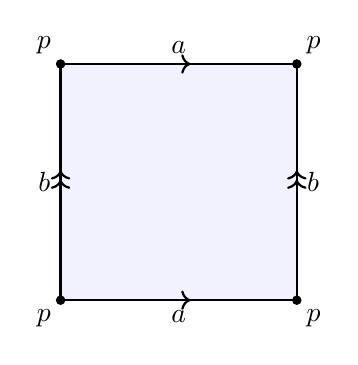
\begin{tikzpicture}[scale=1.5]
        \tikzset{midarrow/.style={decoration={markings, mark=at position 0.55 with {\arrow{>}}},postaction={decorate}}}
        \tikzset{doublemidarrow/.style={decoration={markings, mark=at position 0.55 with {\arrow{>>}}},postaction={decorate}}}

        \fill[blue!5] (0,0) rectangle (2,2);

        \draw[thick, midarrow] (0,0) -- (2,0) node[midway, below] {$a$};
        \draw[thick, midarrow] (0,2) -- (2,2) node[midway, above] {$a$};
        \draw[thick, doublemidarrow] (0,0) -- (0,2) node[midway, left] {$b$};
        \draw[thick, doublemidarrow] (2,0) -- (2,2) node[midway, right] {$b$};

        \filldraw (0,0) circle (1pt) node[below left] {$p$};
        \filldraw (2,0) circle (1pt) node[below right] {$p$};
        \filldraw (0,2) circle (1pt) node[above left] {$p$};
        \filldraw (2,2) circle (1pt) node[above right] {$p$};
    \end{tikzpicture}
    \caption{The fundamental polygon of a torus.}
    \label{fig:torus_polygon}
\end{figure}

Now suppose that 2 sides represented as $b$ are equivalent. 
Then the natural image of such rectangle can be represented as following. 

\begin{figure}[H]
    \centering
    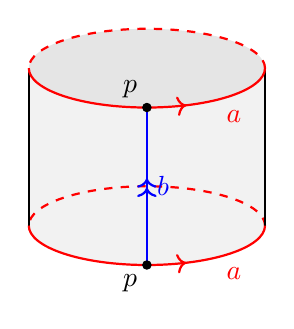
\begin{tikzpicture}[scale=1]
        \tikzset{arrowA/.style={decoration={markings, mark=at position 0.65 with {\arrow{>}}},postaction={decorate}}}
        \tikzset{arrowB/.style={decoration={markings, mark=at position 0.55 with {\arrow{>>}}},postaction={decorate}}}

        \fill[gray!10] (-1.5, 2) arc (180:360:1.5 and 0.5) -- (1.5, 0) arc (360:180:1.5 and 0.5) -- cycle;
        \fill[gray!20] (0,2) ellipse (1.5 and 0.5);

        \draw[thick, red, dashed] (1.5, 2) arc (0:180:1.5 and 0.5);
        \draw[thick, red, dashed] (1.5, 0) arc (0:180:1.5 and 0.5);

        \draw[thick] (-1.5, 0) -- (-1.5, 2);
        \draw[thick] (1.5, 0) -- (1.5, 2);

        \draw[thick, red, arrowA] (-1.5, 2) arc (180:360:1.5 and 0.5) node[pos=0.7, below right] {$a$};
        \draw[thick, red, arrowA] (-1.5, 0) arc (180:360:1.5 and 0.5) node[pos=0.7, below right] {$a$};

        \draw[thick, blue, arrowB] (0, -0.5) -- (0, 1.5) node[midway, right] {$b$};

        \filldraw[black] (0, 1.5) circle (1.5pt) node[above left] {$p$};
        \filldraw[black] (0, -0.5) circle (1.5pt) node[below left] {$p$};

    \end{tikzpicture}
    \caption{The cylinder formed by identifying the edges $b$ of the fundamental polygon.}
    \label{fig:torus_cylinder}
\end{figure}

Now, do same thing to the both side $a$ also. 

\begin{figure}[H]
    \centering
    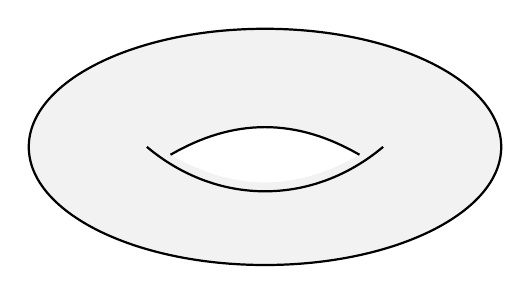
\begin{tikzpicture}[scale=1]
        % 화살표 스타일 정의
        \tikzset{arrowA/.style={decoration={markings, mark=at position 0.3 with {\arrow{>}}},postaction={decorate}}}
        \tikzset{arrowB/.style={decoration={markings, mark=at position 0.5 with {\arrow{>>}}},postaction={decorate}}}

        % 1. 바탕색 칠하기 및 투명 구멍 뚫기
        % 윗입술과 똑같이 위로 휘게(bend left) 만들어서 완벽한 '눈' 모양으로 구멍을 뚫어줍니다.
        \fill[gray!10, even odd rule] 
            (0,0) ellipse (3 and 1.5)
            (-1.2, -0.1) to[bend left=30] (1.2, -0.1)  % 위로 휨
            to[bend left=30] cycle;                    % 되돌아오면서 아래로 휨

        \draw[thick] (0,0) ellipse (3 and 1.5);

        \draw[thick] (-1.5, 0) to[bend right=40] (1.5, 0);
        \draw[thick] (-1.2, -0.1) to[bend left=30] (1.2, -0.1);
    \end{tikzpicture}
    \caption{The standard generators $a$ and $b$ on the torus $\mathbb{T}^2$.}
    \label{fig:torus_generators}
\end{figure}

Our goal in this section is generalizing this notions into topological words. 
Let's define and understand bunch of things from now on. 

\newpage 

\begin{defn}{Quotient Map}{quotient map}
    Let $X, Y$ be topological spaces and $p: X \rightarrow Y$ be a surjective map. 
    The map $p$ is said to be a \textit{quotient map} provided a subset $U$ of $Y$ is open in $Y$ 
    if and only if $p^{-1}(U)$ is open in $X$. 
\end{defn}

\begin{rem}{}{7.2}
    Following is the order of strongness of definitions. 
    \[\begin{tikzcd}
    & & & Quotient ~ Map & \arrow[dr, no head] & & \\
    Continuous ~ Map \arrow[r, no head] & \arrow{ur} \arrow{dr} & & & & \arrow[r] & Homeomorphism \\
    & & & Embeddings & \arrow[ur, no head] & &
    \end{tikzcd}\]
    Quotient map is continuous map with surjectivity and Embedding is continuous map with injectivity, and Homeomorphism is continuous map with bijectivity. 
\end{rem}
The if and only if condition above implies that, quotient map $p$ is continuous($\Rightarrow$) and 
if preimage $p^{-1}(U)$ of something $U \subseteq Y$ is open in $X$, then $U$ is open in $Y$.($\Leftarrow$)
\hl{Note that, there aren't any guarantee that image of any open set in $X$ is also open in $Y$.}
We can obtain an alternative way to define quotient maps. 

\begin{defn}{Saturated Set}{saturated set}
    Let $X, Y$ be topological spaces and $p: X \rightarrow Y$ is a surjective map. 
    We say that $C \subseteq X$ is saturated with respect to $p$ if 
    $C$ equals the complete preimage of some subset of $Y$. i.e., $p^{-1}(p(C)) = C$ holds. Equivalently, 
    $C$ contains all $p^{-1}(\{y\})$ such that intersects with $C$. 
\end{defn}

Then now we can say that \hl{$p$ is quotient map if and only if $p$ is continuous and every open saturated set in $X$ map to open set in $Y$.}
We also say that $f: X \rightarrow Y$ is an \textit{open map} if image of open set in $X$ is open in $Y$. 
Then, every surjective continuous open map is quotient map. (First one is stronger notion). 
Before move on, we summarize such confusing concepts in following way. 

\begin{rem}{Continuous, Quotient, Homeomorphism}{7.4} 
    \begin{itemize}
        \item If $f$ is continuous, $U \subseteq Y$ is open $\implies$ complete preimage of $U$ is open in $X$. 
        \item If $f$ is quotient map, there is a bijection between open sets in $Y$ and open complete preimages in $X$. 
        \item If $f$ is Homeomorphism, there is a bijection between open sets in $Y$ and open sets in $X$. 
    \end{itemize}
\end{rem}

Now we can define \textit{quotient topology} and \textit{quotient space} which are main topics in this section. 
\begin{defn}{Quotient Topology}{quotient topology}
    $X$ is a space and $A$ is a set. For any $p: X \rightarrow A$ surjective map, 
    \hl{there exists unique topology of $A$ such that make $p$ be a quotient map}. 
    Such topology is called \textit{quotient topology} induced by $p$. 
\end{defn}

Such topology of $A$ is just collection of $U \subseteq A$ such that $p^{-1}(U)$ is open in $X$. 
It automatically makes that $p$ be a continuous map, and even quotient map. 
Intuitively, surjective map can be imagine as a compression of $X$ into smaller set $A$. 
Above definition states that, there is the unique \lq shape' for $A$ that makes this becomes \lq good' compression. 
Actually the \lq compression' of space $X$ is quite non-trivial in above context. 
We define the \textit{quotient space} in general and see how to describe such compression in topological words. 

\begin{defn}{Quotient Space}{quotient space}
    Let $X$ be a topological space and $X^*$ be a disjoint partition of $X$. 
    We can define the projection $p: X \rightarrow X^*$ in natural manner, which is surjective map. 
    Then \ref{def:quotient topology} says that we can find unique \textit{quotient topology} of $X^*$. 
    With it, $X^*$ is called quotient space of $X$. 
\end{defn}

Then it is not hard to understand that $X^*$ is compressed space of space $X$. 
Each element in $X^*$ is a sort of \textit{representation} of its equivalent classes of elements of $X$. 
So any $U \subseteq X^*$ is collection of \textit{equivalent classes} and its preimage $p^{-1}(U)$ is open. 

As we stated in first of this section, now we can generalize the constructing torus from 2D rectangle. 
Let 
\[X = [0,1] \times [0,1]\]
Then we can define $X^*$ by: 
\[X^* = \begin{cases}
    \{(x, y)\} & (x,y) \in (0,1) \times (0,1) \\
    \{(0, y), (1, y)\} & y \in (0,1) \\
    \{(x, 0), (x, 1)\} & x \in (0, 1) \\
    \{(0, 0), (0, 1), (1, 0), (1, 1)\}
\end{cases}\]

Then $X^*$ becomes a torus and we can pull-back open sets on torus into open sets on rectangle. 
We state 2 theorems related to continuity on quotient maps. 

\newpage 

\begin{thm}{Continuity of Quotient Map - Mapping Out}{7.7}
    Let $p: X \rightarrow Y$ be a quotient map. 
    Let $Z$ be a space and let $g: X \rightarrow Z$ be a map such that constant on each $p^{-1}(y)$ for $y \in Y$. 
    Then, $g$ induces a map $f: Y \rightarrow Z$ such that $f \circ p = g$. 
    $f$ is continuous if and only if $g$ is continuous, $f$ is quotient map if and only if $g$ is quotient map.
\end{thm}

\begin{center}
\begin{tikzcd}[column sep=huge, row sep=huge, ampersand replacement=\&]
    X \arrow[d, "p"'] \arrow[rd, "g"] \\
    Y \arrow[r, dashed, "f"] \& Z
\end{tikzcd}
\end{center}

\begin{proof}
    $f$ can be well-defined as following way: 
    \[f: y \mapsto g\left( p^{-1}(y) \right)\]
    Then for any $x \in X$, 
    \[f \circ p (x) = g(p^{-1}p(x)) = g(x)\]
    Then it is clear that if $f$ is continuous(quotient map), then $g$ is continuous(quotient map). 
    Now suppose that $g$ is continuous. Let $U$ be any open set in $Z$. 
    Then, $g^{-1}(U)$ is open in $X$. However, $g^{-1}(U)$ is complete preimage of some subset $V$ in $Y$ so $p^{-1}(V) = g^{-1}(U)$. 
    Since $p$ is quotient map, $V$ is open in $Y$. However, $V = p \circ g^{-1}(U) = f^{-1}(U)$ is open in $Y$, so $f$ is continuous.  
\end{proof}

\begin{cor}{}{7.8}
    Let $g: X \rightarrow Z$ be a surjective continuous map. Let $X^*$ be the following 
    collection of subsets of $X$: 
    \[X^* = \{g^{-1}(z) \mid z \in Z\}\]
    Give $X^*$ the quotient topology. 
    \begin{itemize}
        \item The map $g$ induces a bijective continuous map $f: X^* \rightarrow Z$, which is a homeomorphism if and only if $g$ is a quotient map. 
        \begin{center}
        \begin{tikzcd}[column sep=huge, row sep=huge, ampersand replacement=\&]
            X\arrow[d, "p"'] \arrow[rd, "g"]\\
            X^* \arrow[r, "f", dashed, no head] \& Z 
        \end{tikzcd}
        \end{center}
        \item If $Z$ is Hausdorff, so is $X^*$.  
    \end{itemize}
\end{cor}

\begin{proof}
    Since $g$ is surjective, $f = g \circ p^{-1}$ clearly forms the bijection between $X^*$ and $Z$. 
    Suppose that $f$ is a homeomorphism and $g^{-1}(U)$ is open for some subset $U$ of $Z$. 
    Since $f$ is bijection, there exists $V$ in $X^*$ such that $f(V) = U$. 
    Then by definition of $f$, $p^{-1}(V) = g^{-1}(U)$. So $p^{-1}(V)$ is open in $X$, implies that $V$ is open in $X^*$. 
    Since $f$ is homeomorphism, $U$ is open in $Z$. 
    Suppose that $g$ is a quotient map. Then for any open set $U$ in $X$, 
    $p^{-1}(U)$ and $g^{-1}(U)$ both are open in $X^*, Z$ respectively. 
    However, they bijects via $f$, so $f$ is homeomorphism. 
    If $Z$ is Hausdorff, $X^*$ is clearly Hausdorff. 
\end{proof}

\begin{rem}{Intuition about this section}{intuition-quotient map}
    This section is related with \ref{def:evenly covered, covering map} section. 
    At the beginning of this section, we introduce the example that forms torus from rectangle. 
    Under the very definition, the notion \lq fold the space' is bit un-clear. 
    But actually, all the definitions in this section is generalization of \lq folding' spaces. 
    
    First of all, quotient map is \hl{folding}. When we fold something, the continuious and 
    surjectivity is clear. 
    One misterious part is that $p^{-1}(U)$ is open in $X$, then $U \subseteq Y$ is open in $Y$.
    Suppose that there is a shape in folded paper. 
    And we unfold the paper, then obtain some unfolded shapes. 
    That is $p^{-1}(U)$, if it is open, then folded shape becomes open is natural. 

    Now see the conclusion in this section \ref{cor:7.8}. 
    $X$ is rectangle $Z$ is torus, and $X^*$ is the blueprint or description how we fold the rectangle. 
    Bit formally, it is actually description of \lq equivalent classes' of $X$. (Glued structure) 
    Hence, \ref{cor:7.8} says that we can observe that folding rectangle as described at the first of this 
    section is acutally homeomorphic to torus. 
\end{rem}

\newpage 

\section{Connected Spaces}

From now on, our main focus is on defining and analyzing \lq good' shapes and spaces in general. 
First of all, we can imagine the good properties in $\BR^n$ for example, \textit{Maximum Value Theorem, Intermediate Value Theorem, Uniform Continuity Theorem} so on. 
However, in $\BR$, they holds for closed interval $[a, b]$. So we can imagine that $[a, b]$ is somewhat good-shaped subspace of the good space $\BR$. 
Since the condition for \lq good' can be differ for each properties, so we want to generalize them as much as possible. 
The first concept is quite natural, which is called \textit{connectedness}. 

\begin{defn}{Seperation and Connected}{seperation and connected}
    Let $X$ be a topological space. 
    We say that $U, V$ is a \textit{seperation} of $X$ if 
    $U, V \neq \emptyset, X = U \cup V$ and $U, V$ are disjoint open set in $X$. 
    If such $U, V$ are not exists in $X$, then we say that $X$ is \textit{connected} space. 
\end{defn}

\hl{Connectedness is obviously topological invariant. i.e., any Homeomorphism preserves the connectivity.} 
This is clear since any Homeomorphisms preserves the seperation. 
We can define connected space slightly differently. 

\begin{lem}{}{8.2}
    $X$ is connected if and only if clopen sets in $X$ are only the trivial ones(i.e., if $A \subseteq X$ is both closed and open, then $A = \emptyset$ or $X$). 
\end{lem}

\begin{proof}
    Existance of clopen set is equivalent to existance of seperation of $X$. 
\end{proof}

\begin{lem}{Subspace Connectivity}{subspace connectivity}
    If $Y$ is a subspace of $X$, a seperation of $Y$ is a pair of disjoint nonempty sets $A$ and $B$ whose union is $Y$, 
    neither of which contains a limit point of the other. 
    The space $Y$ is connected if and only if there exists no seperation of $Y$. 
\end{lem}

\begin{proof}
    Suppose that $Y$ is not connected, then there exists $A, B \neq \emptyset$, $A \cup B = Y$ and $A, B$ are open in $Y$. 
    Then, $A, B$ are also closed in $Y$. So, by \ref{thm:thm_3.6}, 
    \[A = \text{ closure of $A$ in $Y$ } = \overbar{A} \cap Y\]
    And similarly for $B$, we can obtain that $A, B$ contains all of its limit points in themselves. So, $A, B$ is the seperation of $Y$. 
    Suppose that $A, B$ are a seperation of $Y$. 
    Then we can obtain $A, B$ are both closed and open in $Y$, so $Y$ is not connected. 
\end{proof}

\hl{Here, we can imagine that not only elements but also a limit point acts role of \textit{connection port} of a set.}
First, we can state the notion of \textit{connection port} of elements as following lemmata. 

\begin{lem}{Connected Subspaces}{connected subspaces}
    If the sets $C$ and $D$ form a seperation of $X$, and if $Y$ is a connected subspace of $X$, 
    then $Y$ lies entirely within either $C$ or $D$.
\end{lem}

\begin{proof}
    Suppose not, then $C \cap Y, D \cap Y \neq \emptyset$ and $(C \cap Y) \cap (D \cap Y) = \emptyset$ and both are open in $Y$, 
    moreover $(C \cap Y) \cup (D \cap Y) = Y$. So, contradiction to $Y$ is connected subspace. 
\end{proof}

\begin{lem}{Connection Port - Elements}{connection port - elements}
    The union of connected subspaces that \textcolor{red}{point in common} is connected. 
\end{lem}

\begin{proof}
    Let $\{A_\alpha\}_{\alpha \in J}$ be a family of connected subspaces of $X$ and there exists $x \in X$ such that $x \in A_\alpha$ for any $\alpha \in J$. 
    Suppose that $\bigcup A_\alpha$ is not connected. Then we can find $\bigcup A_\alpha = C \cup D$ where 
    $C, D$ forms seperation of $\bigcup A_\alpha$. W.L.O.G., $x \in C$. 
    Then, according to \ref{lem:lem:connected subspaces}, every $A_\alpha \subseteq C$ so $D = \emptyset$ which is contradiction. 
\end{proof}

Now we state the notion of connection port of limit points as following theorem. 

\begin{thm}{Connection Port - Limit Points}{connection port - limit points}
    Let $A$ be connected subspace of $X$. For $A \subseteq B \subseteq \overbar{A}$, then
    $B$ is connected subspace. 
\end{thm}

\begin{proof}
    Suppose that $B$ is not connected. Then, we can find seperation $U, V$ of $B$ such that 
    $U$ contains all its limit points in $B$ and $V$ also. However since $A \subseteq B$, according to \ref{lem:connected subspaces}
    $A$ entirely in $U$ without loss of generality. 
    Then all elements in $V$ is $B \setminus A \subseteq A'$. But they are limit points of $A \subseteq U$, contradiction. 
\end{proof}

Now we'll see important results for connected spaces. The big question is, \hl{what preserves the connectedness?}

\begin{thm}{Continuous Map Preserves Connectedness}{continuous map preserves connectedness}
    The image of connected set under continuous map is connected. 
\end{thm}

\begin{proof}
    Let $f: X \rightarrow Y$ is continuous map and $X$ is connected space. 
    For convenience, let $Y = \Im(X)$. 
    If $Y$ is not connected, there are $U, V$ forming seperation of $Y$. 
    Since they are open, $f^{-1}(U), f^{-1}(V)$ also open in $X$. 
    And they are non-empty and disjoint partition of $X$, contradiction to $X$ is connected. 
\end{proof}

\begin{thm}{Finite Cartesian Product of connected spaces}{finite cartesian product of connected spaces}
    A finite Cartesian product of connected spaces is connected.
\end{thm}

\begin{proof}
    It is enough to show that if $X, Y$ are connected spaces, then $X \times Y$ is connected. 
    Pick one point $a \times b$ in $X \times Y$. For any $x \in X$, since $x \times Y \cong Y$ and $X \times b \cong X$, 
    both of $x \times Y, X \times b$ are connected. Then \ref{lem:connection port - elements} implies that 
    following subspace is connected: 
    \[T_x = (X \times b) \cup (x \times Y)\]
    Now, form the union $\bigcup_{x \in X} T_x$ then this is also connected since $a \times b \in T_x$ for any $x \in X$ and then \ref{lem:connection port - elements}. 
    However, $\bigcup_{x \in X}T_x = X \times Y$. So $X \times Y$ is connected. 
\end{proof}

Here are some interesting results. As we refered in \ref{prop:box topology versus product topology}, 
when we consider the arbitrary cartesian products, the connectedness depends on what topology we take for the space. 

\begin{thm}{Box Topology and Product Topology, in connectedness}{8.9}
    Let $\{X_\alpha\}_{\alpha \in J}$ is family of connected spaces. 
    $\prod_{\alpha \in J}X_\alpha$ is connected under product topology, but not always true under box topology. 
\end{thm}

The example is quite tricky. We can imagine $\BR^\omega$ as a set of sequences on $\BR$. 
Then, we can categorize such sequences by: 
\[A: \text{ Bounded sequences }, \quad B: \text{ Unbounded sequences}\]
Then $A \cap B = \emptyset$, $A \cup B = \BR^{\omega}$. 
Now we claim that $A, B$ both are open. 
For sequence $\{x_n\}_{n \in \BN}$, construct 
\[U = (x_1 - 1, x_1 + 1) \times (x_2 - 1, x_2 + 1) \times \cdots\]
Then $U$ is open in box topology, and $U \subseteq A$ if $\{x_n\}$ is bounded, and $U \subseteq B$ if $\{x_n\}$ is unbounded. 
So $A, B$ both are open and $\BR^{\omega}$ is not connected. 
Actually this example shows that second part of \ref{thm:8.9}. 
\begin{proof}
    Choose $(x_\alpha)_{\alpha \in J}$ in $\prod X_\alpha$. 
    We can define $Y$ by set of $(y_\alpha)_{\alpha \in J}$ such that $y_\alpha \neq x_\alpha$ for finitely many $\alpha \in J$. 
    Then, we can define $X_K$ by $\prod H_\alpha$ such that $H_\alpha = X_\alpha$ if $\alpha \in K$ and $H_\alpha = \{x_\alpha\}$ if not. 
    Then $X_K \cong \prod_{\alpha \in K}X_\alpha$ Here if $K$ is finite, then $\prod_{\alpha \in K} X_\alpha$ is connected by \ref{thm:finite cartesian product of connected spaces} 
    and so for $X_K$. 
    Note that $Y = \bigcup_{\forall K \subseteq J, |K| < \infty} X_K$ and each $X_K$ has common point 
    $(x_\alpha)$. So $Y$ is connected. 
    Now suppose any basis element $\prod_{\alpha \in L, |L| < \infty} U_\alpha$ for $\prod X_\alpha$. 
    In such basis element, we can always find 
    \[(z_\alpha) = \begin{cases}
        x_\alpha & \alpha \notin L \\
        z_\alpha & \alpha \in L
    \end{cases}\]
    Then it is clear that $(z_\alpha) \in \prod_{\alpha \in L, |L| < \infty} U_\alpha$ and $(z_\alpha) \in Y$. 
    So, every basis of $\prod X_\alpha$ intersects $Y$. Means that every points of $\prod X_\alpha$ is limit points of $Y$, 
    implies that $\overbar{Y} = \prod X_\alpha$. However $Y$ is connected, so $\overbar{Y}$ also connected by \ref{thm:connection port - limit points}. 
    So $\prod X_\alpha$ also connected. 
\end{proof}

\newpage 

\section{Connected Subspaces of The Real Line}

In this section, we state full-of intuitive parts about connectedness. 
We intuitively knows that any intervals and rays are connected in $\BR$. 
Such connected sets in $\BR$ has \lq good' properties, like \textit{intermediate value theorem}. 
Our goal is find the general condition that makes our space holds \textit{intermediate value theorem}, like $\BR$. 
And also, state another fully intuitive notion called \textit{path connected}. 

\begin{defn}{Linear continuum}{linear continuum}
    A simply ordered set $L$ non-empty is called a \textit{linear continuum} if following holds: 
    \begin{enumerate}
        \item $L$ has the least upper bound property.
        \item If $x < y$, exists $z$ such that $x < z < y$. 
    \end{enumerate}
    Where least upper bound property means that, 
    if $A \subseteq L$ is bounded above, then $\sup A \in L$. 
\end{defn}

\hl{This is the target property that our general space behaviors like $\BR$ (in connectedness' perspective).}
First $\BR$-like behavior is following. 

\begin{thm}{Convex Connectedness}{convex connectedness}
    Let $L$ is a linear continuum with ordered topology. \textit{Any convex set $Y$ in $L$ is connected}. 
    So, $L$ itself, intervals, and rays are connected. 
\end{thm}

\begin{proof}
    Suppose that our convex set $Y \subseteq L$ is not connected. 
    Then $Y$ has a seperation $A, B$. 
    Let's choose $a \in A, b \in B$ and $a < b$ withour loss of generality. 
    Since $Y$ is convex, $[a,b] \subseteq Y$. 
    Let's denote 
    \[A_0 = [a,b] \cap A, \quad B_0 = [a,b] \cap B\]
    However, $[a,b] \subseteq Y \subseteq L$ also supspace and $A_0, B_0$ are non-empty open sets in $[a, b]$, which union is $[a,b]$. 
    So $A_0, B_0$ forms seperation of $[a, b]$.
    Now, let $x = \sup A_0$. This is well-defined since $A_0$ is bounded and $L$ is linear continuum. 
    And $a \leq x \leq b$, so $x \in [a,b]$. Suppose that $x \in B_0$. 
    Since $B_0$ is open, we can find small open interval for $x$ in $B_0$. 
    See it partly, we obtain $(d, x] \subseteq B_0$. Then $d$ is smaller upperbound than $x$, contradiction. 
    Vice versa, $Y$ is connected. 
\end{proof}
Now it's time to generalize one of the famous theorem in real analysis, which is \textit{intermediate value theorem}. 
\hl{The condition is much generalized, $f$ is continuous, $X$ is connected, $Y$ is order space. }
\begin{thm}{The Intermediate Value Theorem}{IVT}
    Let $f: X \rightarrow Y$ be a continuous map where $X$ is connected and $Y$ is order space. 
    For $a, b \in X$, if $f(a) < r < f(b)$ then there exists $c \in X$ such that $f(c) = r$. 
\end{thm}

\begin{proof}
    Suppose that such $c$ is not exists. 
    Then, $r \notin \Im(X)$ so we can seperate $\Im(X)$ by 
    \[A_0 = \Im(X) \cap (-\infty, r), \quad B_0 = \Im(X) \cap (r, \infty)\]
    Since $A_0, B_0$ is open in $\Im(X)$ and non-empty disjoint, 
    they are seperation of $\Im(X)$. However, the image of connected space under continuous map is connected by \ref{thm:continuous map preserves connectedness}.
    So this is contradiction, and such $c$ is exists. 
\end{proof}

Now we define another version of connectedness, which is called \textit{path connected}. 
This is drawable concepts, but not exactly equivalent to what we defined. 

\begin{defn}{Path Connected}{path connected}
    Let $X$ be a topological space. We define a \textit{path} between $x, y \in X$ by a continuous mapping 
    $f: [a, b] \rightarrow X$ such that $f(a) = x, f(b) = y$. Where $[a, b] \subseteq \BR$. 
    $X$ is called \textit{path connected} if for every $x, y \in X$, there exists a path from $x$ to $y$. 
\end{defn}

\begin{thm}{Path Connected Implies Connected}{path connected implies connected}
    If $X$ is path connected space, then $X$ is connected space. 
\end{thm}

\begin{proof}
    Suppose that $X$ is not connected so there is a seperation $A, B$ of $X$. 
    Then since every path is image of convex(so, connected) space, \textit{path is connected}. 
    So by \ref{lem:connected subspaces}, path is entirely in $A$ or $B$. 
    Then, we can't find a path between $a \in A$ and $b \in B$, contradiction to $X$ is path connected. 
    So, $X$ is connected.
\end{proof}

\begin{prop}{Connected Does Not Implies Path Connected}{connected does not implies path connected}
    Let $S = \{x \cdot \sin(1/x) \mid 0 < x \leq 1\}$. $\overbar{S}$ is connected but not path connected. 
\end{prop}

\begin{proof}
    Since $S$ is image of $(0, 1]$ under continuous map, so $S$ is connected. This implies that $\overbar{S}$ is connected by \ref{thm:connection port - limit points}. 
    Note that $\overbar{S} = S \cup (0 \times [-1, 1])$. 
    There is not any path between $a \in S, b \in 0 \times [-1, 1]$. 
    If there exists a path, $f: [0, 1] \rightarrow \overbar{S}$ such that $f(0) = b$ and $f(1) = a$ is continuous. 
    However, it oscillate in $[-1, 1]$ near $x = 0$, continuity is not hold near $x = 0$. 
\end{proof}

\newpage 

\section{Compact Space}

When we say something is \lq compact', it means that \lq Wow, that's very good or suitable'. According to our textbook page 161, Munkres\cite{munkres}
refer good historical development of the word \lq compact' in topology. 
First, in $\BR$, we observe that any closed interval has very good properties like 
uniform continuity theorem and maximum value theorem. 
After that, mathematicians like Weierstrass observe that every infinite subsets of $[a, b]$ has a limit point. 
Later, finally we find the core generalization via open coverings. We begin with define open covering of space. 

\begin{defn}{Open Covering}{open covering}
    A family $\CA$ of subsets of $(X, \CT)$ is called \textit{open covering} of $X$ if 
    every $A \in \CA$ is open and $\bigcup_{A \in \CA} A = X$. 
\end{defn}

With this definition, we define general \textit{compact} in topological spaces. 

\begin{defn}{Compact}{compact}
    $X$ is said to be \textit{compact} if for any open covering $\CA$ of $X$ contains \textit{finite subcollection} that also covers $X$. 
\end{defn}

You might realize that it is hard to specify given space is compact. To decide that given space is \textit{not} compact, 
we tries to find proper open covering that we never find finite subcovering from there. Often 
choose \textit{sequential} covering such that decreases, so if there exists finite subcovering, 
some contradiction occurs. For example, following open covering for $(0,1]$ with standard topology shows this: 
\[\{\left(1/n, 1\right] \mid n \in \BN\} \implies (0,1] \text{ is not compact }\]
We can state some lemmata between previous concepts and compactness. 

\begin{lem}{Compactness under Union and Intersection}{compact union intersection}
    Finite union of compact subspaces are compact. Arbitrary intersections of compact subspaces in \textit{Hausdorff} space is compact. 
\end{lem}

\begin{lem}{Subspace Compactness}{subspace compactness}
    Let $Y$ be a subspace of $X$. $Y$ is compact if and only if 
    every open covering of $Y$ in $X$ contains a finite subcovering of $Y$. 
\end{lem}

\begin{thm}{Closed in Compact is Compact}{closed in compact is compact}
    Closed subspace of compact space is compact. 
\end{thm}

\begin{thm}{Compact in Hausdorff is Closed}{compact in Hausdorff is closed}
    Compact subspace of Hausdorff space is closed.
\end{thm}

\begin{proof}
    Let $X$ be a Hausdorff space and $C$ is subspace of $X$ which is compact. 
    Then, we'll show that $X \setminus C$ is open in $X$. 
    Choose any $x \in X \setminus C$. 
    Then for any $y \in C$, since $X$ is Hausdorff, we can find pair of disjoint open neighborhood $U_x, U_y$ with respect to $x, y$. 
    We collect all of this into: 
    \[\CA = \{U_y \mid y \in C\}\]
    Then since this forms a open covering of $C$ in $X$, we can apply \ref{lem:subspace compactness} and 
    obtain finite subcovering of $C$: 
    \[\CA' = \{U_{y_1}, \cdots, U_{y_n}\}\]
    We have its pair elements $U_{x}^1, \cdots, U_{x}^n$ and 
    \[U = \bigcap_{i \in [n]} U_{x_i} \implies \text{ open neighborhood of $x$ disjoint with $C$ }\]
    So, $U \subseteq X \setminus C$, implies that $X \setminus C$ is open in $X$. 
\end{proof}

We bring some useful features in above proof into following lemma. This will be appear in sections about seperation axioms. 

\begin{lem}{}{10.7}
    If $Y$ is a compact subspace of Hausdorff space $X$ and $x \notin Y$, 
    then there exists two disjoint open sets $U$ and $V$: 
    \[U \text{ is neighborhood of $x$ }, \quad Y \subseteq V\]
\end{lem}

Next few theorems construct the connection between continuous map and homeomorphisms with compactness.

\begin{thm}{Continuous Map Preserves Compactness}{continuous preserves compact}
    The image of compact space under continuous map is compact. 
\end{thm}

\begin{proof}
    Straight forward, so omitted. 
\end{proof}

\begin{cor}{Compactness is Absolute}{compact is absolute}
    Let $Y$ be the subspace of $X$. If $K$ is compact in $Y$, then $K$ also compact in $X$. 
\end{cor}

\begin{proof}
    Natural inclusion $f: Y \hookrightarrow X$ is continuous. 
    Since continuity preserves compactness, $f(K) = K \subseteq X$ also compact. 
\end{proof}

\begin{thm}{From Compact into Hausdorff}{}
    Let $f: X \rightarrow Y$ be a bijective continuous map. If $X$ is compact and $Y$ is Hausdorff then $f$ is a homeomorphism. 
\end{thm}

\begin{proof}
    Only thing we need to do is that show $f^{-1}$ is continuous. 
    Then it is enough to show that, image of closed set in $X$ is also closed in $Y$. 
    First, if $A \subseteq X$ is closed, then it is compact by \ref{thm:closed in compact is compact}. 
    However, image of compact subspace under continuous map is also compact by previous theorem. 
    Finally, compact subspace $\Im(A)$ under $f$ in Hausdorff space $Y$ is closed by \ref{thm:compact in Hausdorff is closed}. 
\end{proof}

Now we prove some important and quite non-trivial statements. 

\begin{lem}{Tube Lemma}{tube lemma}
    Let $X \times Y$ be a product space where $Y$ is compact. 
    If $N$ is open set of $X \times Y$ containing $x_0 \times Y$ for some $x_0 \in X$, 
    then $N$ contains some \textit{tube} $W \times Y$ about $x_0 \times Y$, where $W$ is a neighborhood of $x_0$ in $X$. 
\end{lem}

\begin{proof}
    Since $N$ is an open set of $X \times Y$, we can denote $N$ is a union of basis element $\CT_X \times \CT_Y$. 
    So, denote 
    \[N = \bigcup_{\alpha \in J} (U_\alpha \times V_\alpha), \quad U_\alpha \in \CT_X, \quad V_\alpha \in \CT_Y\]
    Now here, since $x_0 \times Y \subseteq N$, $\{V_\alpha \mid \alpha \in J, x_0 \in U_\alpha \}$ 
    is open covering of $Y$ and so we can find finite subcovering of $Y$ by 
    \[\{V_i \mid i \in [n], x_0 \in U_i \} \text{ such that } \bigcup_{i \in [n]} V_i = Y\]
    Then, we construct 
    \[W = \bigcap_{i \in [n]} U_i \implies W \text{ is neighborhood of $x_0$ in $X$}\]
    Then it is clear that $W \times Y \subseteq N$. 
\end{proof}

\begin{thm}{Product of Finite Compact is Compact}{product of finite compact is compact}
    The product of finitely many compact space is compact. 
\end{thm}

\begin{proof}
    If is sufficient to show that if $X, Y$ is compact then $X \times Y$ is compact. 
    Let $\CA$ be any open covering of $X \times Y$. 
    Then for any fixed $x_0 \in X$, $x_0 \times Y$ is homeomorphic to $Y$ and so compact. 
    By \ref{lem:subspace compactness}, $x_0 \times Y$ is compact subspace of $X \times Y$ and 
    $\CA$ is a open covering of $x_0 \times Y$, so we can find finite subcovering $A_1, \cdots, A_n \in \CA$ such that 
    $x_0 \times Y \subseteq \bigcup A_i = N$. 
    Then according to \ref{lem:tube lemma}, we can find $W_{x_0} \times Y \subseteq N$ such that $W$ is neighborhood of $x_0$ in $X$. 
    Do this for every $x_0 \in X$ then collect 
    \[\{W_x \mid x \in X\} \implies \text{ open covering of $X$ } \implies \text{Finite subcovering } \{W_{x_1}, \cdots, W_{x_m}\}\]
    Then, 
    \[\{W_{x_i} \times Y \mid i \in [m]\} \implies \text{Finite Subcovering of $\CA$ of $X \times Y$}\] 
    This completes the proof.
\end{proof}

\begin{thm}{Tychonoff Theorem}{Tychonoff theorem}
    Product of arbitrary many compact spaces is compact. 
\end{thm}

\begin{proof}
    We prove this later.
\end{proof}

Finally, we propose another criterion for space to be compact. 

\begin{defn}{Finite Intersection Property}{finite intersection property}
    A collection $\CC$ of subsets of $X$ is said to have the \textit{finite intersection property} if for 
    every finite subcollection 
    \[\{C_1, \cdots, C_n\}\]
    of $\CC$, the intersection $C_1 \cap \cdots \cap C_n$ is nonempty. 
\end{defn}

\begin{thm}{Finite Intersection Property Criterion}{finite intersection property criterion}
    $X$ is compact if and only if every collection $\CC$ of \textit{closed subsets} in $X$ having finite intersection property,
    then $\bigcap_{C \in \CC} C \neq \emptyset$. 
\end{thm}

\begin{proof}
    Suppose that $X$ is compact and $\CC$ is a collection of closed subsets which having finite intersection property. 
    Means that for any finite subfamily, there intersection is non-empty. 
    We forms 
    \[\CA = \{X \setminus C \mid C \in \CC\}\]
    Suppose that $\bigcap_{C \in \CC} C = \emptyset$, then $\CA$ become open covering of $X$. hence we can find finite subcovering. 
    Which means that 
    \[A_1 \cup \cdots \cup A_n = X \implies X \setminus (C_1 \cap \cdots \cap C_n) = X\]
    implies that 
    \[C_1 \cap \cdots \cap C_n = \emptyset\]
    This is contradiction, hence $\bigcap_{C \in \CC} C \neq \emptyset$. 

    Suppose that later condition holds. 
    Given $\CA$ be any open covering of $X$. 
    Then construct 
    \[\CC = \{X \setminus A \mid A \in \CA\}\]
    This become family of closed sets. If it has no finite intersection property, we can find 
    \[(X \setminus A_1) \cap \cdots \cap (X \setminus A_n) = \emptyset \implies A_1, \cdots, A_n \text{ is finite subcovering $\implies$ $X$ is compact}\]
    If it holds finite intersection property, contradiction to $\CA$ is covering of $X$.
\end{proof}

\newpage 

\section{Metric and Metric Topology}

Before moving on to the compactness of Euclidean spaces, it is good time to define the 
general notion of distance, which is called \textit{metric} and topology induced by it. 
$\BR$ is very intuitive space for us and we learned so far about $\BR$. 
In many theories including topology, sometimes they behaves like \textit{meta-theory} of our domain. 
The notion of \textit{metric} is sort of that. 
The \textit{metric}, general notion of distance is defined as following. 

\begin{defn}{Metric}{metric}
    A \textit{metric} on a set $X$ is a function 
    \[d: X \times X \rightarrow \BR\]
    with following axioms: 
    \begin{enumerate}
        \item $d(x, y) \geq 0$ for every $x, y \in X$ and $d(x, y) = 0 \iff x = y$. 
        \item $d(x, y) = d(y, x)$ for any $x, y \in X$. 
        \item $d(x, y) + d(y, z) \geq d(x, z)$ for any $x, y, z \in X$.
    \end{enumerate}
\end{defn}

\begin{notn}{Open Ball}{open ball}
    Given metric $d$ of $X$ and $\varepsilon > 0$, we denote 
    \[B_d(x, \varepsilon) = \{y \mid d(x, y) < \varepsilon\}\]
    and it is called \textit{$\varepsilon$-ball centered at $x$}. When $d$ is trivial in context, we denote $B(x, \varepsilon)$ often. 
\end{notn}

This two notion is very familiar from real analysis course. However, note that metric is 
defined on the arbitrary set $X$. So one natural further step is that, 
when metric on a set $X$ is given, what is the natural topology for $X$ induced by the metric? 

\begin{defn}{Metric Topology}{metric topology}
    Let $d$ be a metric on a set $X$. Topology generated by \textit{collection of all $\varepsilon$-balls in $X$} is called the \textit{metric topology induced by $d$}. 
    i.e., 
    \[\CB = \{B_d(x, \varepsilon) \mid x \in X, \varepsilon > 0\}\]
\end{defn}

This is well-defined since if $x \in B_1 \cap B_2$ where $B_1 = B(y, \varepsilon_1), B_2 = B(z, \varepsilon_2)$ then 
we can find $\delta = \min \left(\varepsilon_1 - d(x, y), \varepsilon_2 - d(x, z)\right)$ then $x \in B(x, \delta) \subseteq B_1 \cap B_2$. 

Again also natural question is occuring. Since we show that given metric can induce natural topology of $X$, 
we want to ask the reverse: 
\begin{center}
    \textit{When $(X, \CT)$ is given, can we find proper metric $d$ that induces the topology of $X$?}
\end{center}
It's a sort of important question, and indeed, very strong condition in topology. 
\begin{defn}{Metrizable}{metrizable}
    Topological space $X$ is said to be \textit{metrizable} if there exists a metric $d: X \times X \rightarrow \BR$ such that 
    induces the topology of $X$. A \textit{metric space} is a metrizable space $X$ together with a explicit metric $d$ that induces that topology of $X$.  
\end{defn}
Once we can prove that $X$ is metrizable, then it is \textit{almost visualizable}, i.e., it becomes 
very intuitive and nature space for us. So many intuitive lemmata guaranteed on metrizable space, 
and also proving $X$ is metrizable is important problem. Since they are main branch of topological theory, 
we'll see that in later section. 
Now we'll do almost recap from analysis course. 

\begin{defn}{Bounded, Diameter}{bounded, diabmeter}
    $X$ is a metric space with metric $d$. $A \subseteq X$ is said to be bounded if 
    there exists $M \in \BR$ such that 
    \[\forall a_1, a_2 \in A, \quad d(a_1, a_2) \leq M\]
    If $A$ is bounded and nonempty, we can define \textit{diameter} of $A$ by 
    \[\text{diam}(A) = \sup \{d(a_1, a_2) \mid a_1, a_2 \in A\}\]
\end{defn}

\begin{thm}{Standard Bounded Metric}{standard bounded metric}
    $X$ is a metric space with metric $d$. We define $\overbar{d}: X \times X \rightarrow \BR$ by 
    \[\overbar{d} : (x, y) \mapsto \min \{d(x, y), 1\}\]
    Then $\overbar{d}$ is a metric and it induces the same topology as $d$. This is called \textit{standard bounded metric} corresponding to $d$. 
\end{thm}

\begin{defn}{Norm, Euclidean Metric, Square Metric}{norm, euclidean metric, square metric}
    Given $\mathbf{x} = (x_1, \cdots, x_n) \in \BR^n$, we define \textit{norm} of $\mathbf{x}$ by 
    \[\norm{x} = (x_1^2 + \cdots + x_n^2)^{1/2}\]
    We define the \textit{Euclidean metric} $d$ on $\BR^n$ by 
    \[d(\mathbf{x}, \mathbf{y}) = \norm{\mathbf{x} - \mathbf{y}}\]
    We define the \textit{square metric} $\rho$ by 
    \[\rho(\mathbf{x}, \mathbf{y}) = \max \{|x_1 - y_1|, \cdots, |x_n - y_n|\}\]
\end{defn}

\begin{lem}{Comparison of Metrics}{comparison of metrics}
    Let $d, d'$ be two metrics on $X$ and $\CT, \CT'$ be topologies they induce, respectively. 
    $\CT \subseteq \CT'$ if and only if $\forall x \in X$ and $\forall \varepsilon > 0$, there exists $\delta > 0$ such that $B_{d'}(x, \delta) \subseteq B_d(x, \varepsilon)$.  
\end{lem}

\begin{proof}
    $\CT \subseteq \CT'$ if and only if for any basis $x \in B$ of $\CT$ we can find $B' \in \CB'$ such that $x \in B' \subseteq B$. 
    This directly same statements as desired. 
\end{proof}

\begin{cor}{Euclidean Metric and Square Metric on $\BR^n$}{11.9}
    On $\BR^n$, topology generated by Euclidean metric and square metric are same. 
\end{cor}

Now we have the cases what we've seen in section 6 which is arbitrary cartesian product space $\BR^J$. 
When $J$ is infinite index set, the definition of Euclidean metric and square metric is not always well-defined. 
So we now observe how can we generalize that cases and connect with box topology, product topology. 

\begin{defn}{Uniform Metric, Uniform Topology}{uniform metric, uniform topology}
    Let $\mathbf{x} = (x_\alpha)_{\alpha \in J}, \mathbf{y} = (y_\alpha)_{\alpha \in J}$ of $\BR^J$. 
    We define \textit{uniform metric} $\overbar{\rho}$ on $\BR^J$ by 
    \[\overbar{\rho}(\mathbf{x}, \mathbf{y}) = \sup\{\overbar{d}(x_\alpha, y_\alpha) \mid \alpha \in J\}\]
    where $\overbar{d}$ is the standard bounded metric on $\BR$ in \ref{thm:standard bounded metric}. 
    Topology induced by it is called the \textit{uniform topology} of $\BR^J$. 
\end{defn}

\begin{thm}{Product $<$ Uniform $<$ Box in $\BR^J$}{11.11}
    In $\BR^J$, 
    \[\textit{Product topology} \subseteq \textit{Uniform topology} \subseteq \textit{Box topology}\]
    If $J$ is infinite, 
    \[\textit{Product topology} \subset \textit{Uniform topology} \subset \textit{Box topology}\]
\end{thm}

\begin{proof}
    Let $\mathbf{x} = (x_\alpha)_{\alpha \in J}$ and $\mathbf{x} \in \prod U_\alpha$ which is a basis of product topology. 
    So, $U_\alpha$ is non-$\BR$ open subset of $\BR$ in $\alpha_1, \cdots, \alpha_n$ and $U_\alpha = \BR$ for other indices. 
    Since $U_{\alpha_i}$ is open in $\BR$ and $x_{\alpha_i} \in U_{\alpha_i}$, 
    we can find $\varepsilon_i$ such that $B(x_{\alpha_i}, \varepsilon_i) \subseteq U_{\alpha_i}$. 
    Since standard bounded metric induces same topology of $\BR$ as Euclidean metric, we can denote 
    \[B_{\overbar{d}}(x_{\alpha_i}, \varepsilon_i) \subseteq U_{\alpha_i}\]
    Let $\varepsilon = \min\{\varepsilon_1, \cdots, \varepsilon_n\} > 0$. 
    Then we can define $B_{\overbar{\rho}}(\mathbf{x}, \varepsilon)$. It is clear that 
    \[\mathbf{x} \in B_{\overbar{\rho}}(\mathbf{x}, \varepsilon) \subseteq \prod_{\alpha \in J} U_\alpha\]
    So, uniform topology is finer than product topology. 

    Let $\mathbf{x} = (x_\alpha)_{\alpha \in J}$ and $\mathbf{x} \in B_{\overbar{\rho}}(\mathbf{x}, \varepsilon)$. 
    Then we can construct 
    \[U_\alpha = \left(x_\alpha - \frac{1}{2}\varepsilon, x_\alpha + \frac{1}{2}\varepsilon \right)\]
    for each $\alpha \in J$. Then, $\prod U_\alpha$ is basis of box topology such that 
    \[\mathbf{x} \in \prod U_\alpha \in B_{\overbar{\rho}}(\mathbf{x}, \varepsilon)\]
\end{proof}

\begin{thm}{Product Topology is Metrizable}{product topology is metrizable}
    Let $\overbar{d}$ be the standard bounded metric on $\BR$ referred in \ref{thm:standard bounded metric}. 
    Define 
    \[D: (\mathbf{x}, \mathbf{y}) \mapsto \sup \left\{\frac{\overbar{d}(x_i, y_i)}{i}\right\}\]
    where $\mathbf{x}, \mathbf{y} \in \BR^\omega$, set of sequences in $\BR$. (i.e., countable infinite) 
    Then $D$ is a metric that \hl{induces the \textit{product topology} on $\BR^\omega$}. 
\end{thm}

\begin{proof}
    First, we claim that $D$ is a metric of $\BR^\omega$. The metric axioms in \ref{def:metric} (1), (2) is obvious. 
    For any $\mathbf{x}, \mathbf{y}, \mathbf{z} \in \BR^\omega$, since $\overbar{d}$ is a metric of $\BR$,
    \[\overbar{d}(x_i, z_i) \leq \overbar{d}(x_i, y_i) + \overbar{d}(y_i, z_i) \implies \frac{\overbar{d}(x_i, z_i)}{i} \leq \frac{\overbar{d}(x_i, y_i)}{i} + \frac{\overbar{d}(y_i, z_i)}{i} \leq D(\mathbf{x}, \mathbf{y}) + D(\mathbf{y}, \mathbf{z})\]
    for every $i$. So, 
    \[D(\mathbf{x}, \mathbf{z}) \leq D(\mathbf{x}, \mathbf{y}) + D(\mathbf{y}, \mathbf{z})\]
    So $D$ is a metric of $\BR^\omega$. 

    Now we prove that topology induced by $D$ is same with product topology of $\BR^w$. 
    Let $\mathbf{x} = (x_\alpha)_{\alpha \in J}$. First, we choose a basis of topology induced by $D$: 
    \[B_D(\mathbf{x}, \varepsilon) \implies \sup \left\{\frac{\overbar{d}(x_i, y_i)}{i}\right\} < \varepsilon\]
    Then, there exists $m \in \BN$ such that $\varepsilon \cdot m > 1$. So, 
    \[i \geq m \implies \overbar{d}(x_i, y_i) \leq 1 \implies y_i \in \BR\]
    Then we can construct 
    \[\prod U_i , \quad U_i = \begin{cases}
        B(x_i, \varepsilon) & i < m \\
        \BR & i \geq m
    \end{cases}\]
    Then for $\mathbf{y} \in \prod U_i$, 
    \[D(\mathbf{x}, \mathbf{y}) = \max_{1 \leq i < m}\left\{\frac{\overbar{d}(x_i, y_i)}{i}, \frac{1}{m}\right\} < \varepsilon\] 
    So, $\mathbf{x} \in \prod U_i \subseteq B_D(\mathbf{x}, \varepsilon)$. 

    Second, we choose a basis of product topology: 
    \[\mathbf{x} \in \prod U_i, \quad U_i = \begin{cases}
        \text{Open set of $\BR$ that }\neq \BR & U_{i_1}, \cdots, U_{i_n} \\
        \BR & \text{otherwise}
    \end{cases}\]
    Then, we can find $0 < \varepsilon_1, \cdots, \varepsilon_n < 1$ such that 
    \[B_{\overbar{d}}(x_{i_j}, \varepsilon_j) \subseteq U_{i_j}, \quad j \in [n]\]
    Now, let 
    \[\varepsilon = \min \left\{\frac{\varepsilon_1}{i_1}, \cdots, \frac{\varepsilon_n}{i_n}\right\}\]
    Then, $\mathbf{x} \in B_D(\mathbf{x}, \varepsilon) \subseteq \prod U_i$
\end{proof}

\begin{thm}{Subspaces of Metric Space is Metric Space}{11.13}
    Let $X$ be a metric space with metric $d$. 
    If $A$ is subspace of $X$ with subspace topology, $d|_{A \times A}$ is metric of $A$ 
    and it induce that topology. 
\end{thm}

\begin{lem}{Metric Space is Hausdorff}{11.14}
    Metric space is Hausdorff. 
\end{lem}

Once metric is defined, the notion of continuity become more intuitive to us. 
As I mentioned, the formal definition of continuity said that \lq near images are from near domain'. 
The concept \lq near' can be dealt with numerical number in metric space. \lq $\varepsilon$-near images are from $\delta$-near domain elements'. 

\begin{thm}{Continuity on Metrizable Space}{continuity on metrizable space}
    Let $f: X \rightarrow Y$ and $X, Y$ are metrizable with $d_X, d_Y$ respectively. 
    The continuity of $f$ is equivalent to that given any $x \in X$ and $\varepsilon > 0$, 
    there exists $\delta > 0$ such that 
    \[d_X(x, y) < \delta \implies d_Y(f(x), f(y)) < \varepsilon\] 
\end{thm}

In analysis, the sequence is sort of important feature we studied. 
We might want to generalize the concept of sequences and convergence also. 
First one is the relation between limit points and convergent sequence. 

\begin{lem}{The Sequence Lemma}{sequence lemma}
    Let $X$ be a topological space. 
    For $A \subseteq X$, if there is a sequence of points of $A$ converging to $x$, then $x \in \overbar{A}$. 
    The converse holds if $X$ is metrizable. (i.e., if $X$ is metrizable there exists a sequence of points of $A$ such that converges into $x \in \overbar{A}$. )
\end{lem}

\begin{proof}
    Let $\{a_n\}_{n \in \BN}$ converges to $x \in X$. 
    By the definition, for any neighborhood $U$ of $x$ in $X$, 
    there exists $N \in \BN$ such that if $a_n, n \geq \BN$ then $a_n \in U$. This automatically implies that 
    for any neighborhood $U$ of $X$, $U \cap A \neq \emptyset$ so $x \in \overbar{A}$. 

    Let $X$ be metrizable with $d$ and $x \in \overbar{A}$. 
    Then, we can construct 
    \[\{B_d(x, 1/n) \mid n \in \BN\}\]
    becomes sequence of neighborhood of $x$ in $X$. 
    However since $x \in \overbar{A}$, we can find elements of $A$ in each open balls. 
    Let's denote them by $\{a_n\}_{n \in \BN}$. It converges to $x$ in $A$. 
\end{proof}

\begin{thm}{Continuity Preserves Convergence}{Continuity Preserves Convergence}
    If $f: X \rightarrow Y$ is continuous and $\{x_n\}_{n \in \BN} \rightarrow x$ is a convergent sequence in $X$ 
    then $\{f(x_n)\}_{n \in \BN}$ converges to $f(x)$ in $Y$. 
    The converges holds if $X$ is metrizable. 
\end{thm}

\begin{proof}
    The preimage of neighborhood $U$ of $f(x)$ in $Y$ is neighborhood $V$ of $x$ in $X$, so we can find 
    $N \in \BN$ such that $x_n \in N$ for $n \geq V$. So, all of images of them sended into $U$, so $\{f(x_n)\}$ converges to $f(x)$. 

    If $X$ is metrizable and latter condition holds, we'll see the continuity of $f$ by $f(\overbar{A}) \subseteq \overbar{f(A)}$. 
    If $x \in \overbar{A}$, then we can find $\{x_n\}$ in $A$ converges to $x$ since $X$ is metrizable, by \ref{lem:sequence lemma}. 
    Then, $\{f(x_n)\}$ converges to $f(x)$ by the condition. So, $f(x) \in \overbar{f(A)}$. This implies that 
    $f(\overbar{A}) \subseteq \overbar{f(A)}$, $f$ is continuous by \ref{thm:thm_5.5}. 
\end{proof}

As you might realized, we used metrizable property while proving \ref{lem:sequence lemma} however 
\lq not very much' use the power of metrizable spaces. We just used to obtain \hl{sequencially decreasing neighborhood of $x$}. 
So indeed, \ref{lem:sequence lemma} and \ref{thm:Continuity Preserves Convergence} holds on weaker condition. 
It is quite non-trivial definition, but we'll revisit this concept in latter section. 

\begin{defn}{Countable Basis, First Countability}{coutable basis, first Countability}
    A space $X$ is said to have a \textit{countable basis at the point $x$} if there is a countable collection 
    $\{U_n\}_{n \in \BN}$ of neighborhoods of $x$ such that any neighborhood $U$ of $x$ contains at least one of the sets $U_n$. 
    i.e., $\forall U$ neighborhood of $x$, we can find $U_n$ such that $x \in U_n \subseteq U$ from countable many $\{U_n\}$. 
    If $X$ has a countable basis at each points then $X$ satisfy the \textit{first countability axiom}. 
\end{defn}

\begin{rem}{Holds on First Countable Space $X$}{11.19}
    We can replace $B(x, 1/n)$ into $B_n = U_1 \cap \cdots \cap U_n$ for countable basis $\{U_n\}$ of $x$ 
    in proof of \ref{lem:sequence lemma} and so on \ref{thm:Continuity Preserves Convergence}. 
\end{rem}

In analysis, we also dealt with sequence of functions and its convergences. 

\newpage 

\begin{defn}{Uniform Convergence}{uniform convergence}
    Let $\{f_n: X \rightarrow Y\}$ be a sequence of functions from \hl{set $X$ to metric space $Y$ with $d$}. 
    We say that $\{f_n\}$ \textit{converges uniformly} to $f$ and denote $\{f_n\} \rightrightarrows f$ 
    if given $\varepsilon > 0$, there exists $N \in \BN$ such that 
    \[d(f_n(x), f(x)) < \varepsilon\]
    for all $n > N$ and $\forall x \in X$. 
\end{defn}

\begin{thm}{Uniform Limit Theorem}{uniform limit theorem}
    Let $f_n: X \rightarrow Y$ be a sequence of \hl{continuous functions} from topological space $X$ into metric space $Y$. \hl{If $\{f_n\}$ uniformly converges to $f$ then $f$ is continuous.}
\end{thm}

\begin{proof}
    Let $V$ be open in $Y$. For $y_0 \in V$, let $f(x_0) = y_0$. Then we can find $B(y_0, \varepsilon) \subseteq V$. 
    Since $\{f_n\} \rightrightarrows f$, we can find $N \in \BN$ such that $d(f_n(x), f(x)) < \varepsilon/3$ for any $x \in X$. 
    Here, $f_N$ is continuous map, so we can state that $U = f^{-1}_N(B(f_N(x_0), \varepsilon/3))$ is open neighborhood of $x_0$ in $X$. 
    Then for $x \in U$, 
    \[d(f(x), f_N(x)) < \varepsilon/3 \quad \because \text{ uniform continuity }\]
    \[d(f_N(x), f_N(x_0)) < \varepsilon/3 \quad \because x, x_0 \in U\]
    \[d(f_N(x_0), f(x_0)) < \varepsilon/3 \quad \because \text{ uniform continuity }\]
    This implies that if $x \in U$, $d(f(x), f(x_0)) < \varepsilon$ so $x \in U$ implies that $U \subseteq f^{-1}(V)$, so $f^{-1}(V)$ is open in $X$. 
\end{proof}

\begin{rem}{Uniform Metric and Uniform Convergence}{11.22}
    The \textit{uniform metric} is related with \textit{uniform convergence}. 
\end{rem}

Recap, uniform metric on $\BR^J$ is defined by 
\[\overbar{\rho}: (\mathbf{x}, \mathbf{y}) \mapsto \sup \left\{\overbar{d}(x_\alpha, y_\alpha) \mid \alpha \in J\right\}\]
For a set $X$, view $\BR^X$ as collection of $f: X \rightarrow \BR$ and give $\BR^X$ to uniform metric. 
Suppose that $\{f_n\}$, the sequence of elements in $\BR^X$ converges to $f$ with respect to uniform metric. 
We can say that $f_n: X \rightarrow \BR$ uniformly converges to $f$. 

\begin{rem}{Not metrizable}{11.23}
    To show that some space is not metrizable, in many case we show that 
    such space does not holds sequence lemma with some counter example. 
\end{rem}

\newpage 

\section{Compactness with Metric}

Again, the motive of compact space is generally good space to derive. 
For motivation, we state following theorem without proof. 

\begin{thm}{Compact = Closed and Bounded in $\BR^n$}{compact = closed and bounded}
    $A \subseteq \BR^n$ is compact if and only if $A$ is closed and bounded in $\BR^n$ 
    under Euclidean metric or square metric.
\end{thm}

Anyone read this theorem might agree that such space is intuitively, enough good for analysis. 
One good property of compact space is stated in following theorem. 

\begin{thm}{Extreme Value Theorem}{extreme value theorem}
    Let $f: X \rightarrow Y$ be countinuous function where $Y$ is order topology space. 
    If $X$ is compact, then $\exists \, c, d \in X$ such that $f(c) \leq f(x) \leq f(d)$ for any $x \in X$. 
\end{thm}

\begin{proof}
    Since continuous map preserves compactness by \ref{thm:continuous preserves compact}, 
    $f(X) \subseteq Y$ is compact. So, since 
    \[\{(-\infty, a) \mid a \in f(X)\} \implies \text{open cover of $f(X)$}\]
    we can find finite subcovering, 
    \[\{(-\infty, a_1), \cdots, (-\infty, a_n)\} \implies \max\{a_i\} = \sup f(X) = f(d)\]
    Similarly for $\inf f(X)$. 
\end{proof}

From now on, \textit{the most important and useful} theorems will be stated. 
Before moving on, we define one more very intuitive notion: distanct from point-to-set. 
There are few way to define it, however following definition is the most standard one. 

\begin{defn}{Distance from Point to Set}{distance from point to set}
    Let $(X, d)$ be a metric space and $\emptyset \neq A \subseteq X$. 
    For $x \in X$, we can define the \textit{distance} from $x$ to $A$ by 
    \[d(x, A) := \inf \{d(x, a) \mid a \in A\}\]
\end{defn}

\begin{rem}{Distance is Continuous}{12.4}
    For fixed $A$, distance in continuous over $X$. 
\end{rem}

Now here we state one of the most important theorem in this summary note. 

\newpage

\begin{thm}{Lebesgue Number Lemma}{Lebesgue number lemma}
    Let $\CA$ be an open covering of the metric space $(X, d)$. 
    If $X$ is compact then there exists $\delta > 0$ such that 
    each subset of $X$ having diameter less than $\delta$, there exists an element of $\CA$ containing it. 
    Such $\delta$ is called a \hl{Lebesgue number} for the covering $\CA$. 
\end{thm}

\begin{proof}
    Let $\CA$ be an open covering of $X$. 
    If $X \in \CA$, then we can take any $\delta > 0$ to be Lebesgue number. Hence, 
    suppose that $X \notin \CA$ is natural. 

    As $X$ is compact, we can find finite subcovering $\{A_1, \cdots, A_n\}$. 
    Let's define $f: X \rightarrow \BR$ as follow
    \[f: x \mapsto \frac{1}{n} \sum_{i = 1}^{n} d(x, X \setminus A_i)\]
    this is continuous function as each distance is continuous. 
    Hence, the image $f(X)$ is compact in $\BR$ since $X$ is compact. 
    By \ref{thm:extreme value theorem}, we can find minimum $f(x_0) \in f(X)$. 
    Let 
    \[\delta = f(x_0) = \text{ minimum in } f(X)\]
    Since $x_0 \in A_i$ for some $i \in [n]$, $\delta > 0$ holds.

    Now we claim that this $\delta > 0$ be the Lebesgue number. 
    Let $B \subseteq X$ where $\operatorname{diam}(B) < \delta$. 
    For any $b \in B$, 
    \[\delta \leq f(b) = \frac{1}{n} \sum_{i = 1}^{n} d(b, X \setminus A_i) \leq d(b, X \setminus A^*)\]
    It means that, distance between $b$ and $A^*$ is at least $\delta$ we obtained. 
    Hence, 
    \[B \subseteq B(b, \delta) \subseteq A^* \in \CA\]
    Hence, $\delta > 0$ is well-defined Lebesgue number and always exists for any open covering $\CA$ of 
    compact space $X$. 
\end{proof}

Now view $\CA$ as the \textit{collection of open sets} such that as many as enough to cover $X$ totally. 
The Lebesgue number theorem states that, if $X$ is compact space then 
we can assume that any sufficiently small($\delta$-small) subset of $X$ is totally contained in some given open set. 

In compact space another good property also arises which is called \textit{uniform continuous}. 

\begin{defn}{Uniform Continuous}{uniform continuous}
    $f: X \rightarrow Y$ is a continuous map where $X, Y$ are metric space induced by $d_X, d_Y$ respectively. 
    $f$ is uniformly continuous if for any $\varepsilon > 0$, we can find $\delta > 0$ such that 
    \[d_X(x_0, x_1) < \delta \implies d_Y(f(x_0), f(x_1)) < \varepsilon\]
\end{defn}

We describe that the continuity intuitively implies that \textit{near elements(neighborhood) of codomain is from a near elements(neighborhood) of domain}. 
Uniform continuity (1) Explicitly determines the \lq near' via metric $d_X, d_Y$ respectively. (2) Such nearness is \lq globally determined' for $X, Y$ both. 

\begin{thm}{Uniform Continuity Theorem}{uniform continuity theorem}
    Continuous function from compact metric space into general metric space is uniformly continuous.
\end{thm}

\begin{proof}
    Easily proved by \ref{thm:Lebesgue number lemma}. Find $\delta$ from 
    preimage of $\varepsilon/2$-open balls for each element of $Y$. 
    For $x_0 \in X$, image of any $\delta/2$-ball centered by $x_0$ is contained in 
    $\varepsilon/2$-ball. 
\end{proof}

Finally we prove that the uncountablity of real number. We say that $x \in X$ is an \textit{isolated point} of $X$ 
if $\{x\}$ is open in $X$. 

\begin{thm}{Uncountablity of Compact Hausdorff with Non-isolated}{12.8}
    Let $X$ be a nonempty compact Hausdorff space. If $X$ has no isolated points, then $X$ is uncountable. 
\end{thm}

\begin{proof}
    Let $x \in X$ and $U$ be arbitrary chosen nonempty open set of $X$. 
    If $x \in U$, since $x$ is not isolated point, $\{x\} \subset U$ so we can find $x \neq y \in U$. 
    If $x \notin U$, since $U$ is nonempty we can find $x \neq y \in U$. 
    Since $X$ is Hausdorff, we can construct two open sets $W_x, W_y$ distinguishing $x, y$ respectively. 
    Let $V = W_y \cap U$. Again it distinguishes $x$ in $U$ and open. Since $x \in W_x \subseteq X \setminus V$, 
    we can say that $x \notin \overbar{V}$. 

    Let $f: \BN \rightarrow X$ and $f(n) := x_n$. 
    Let $V_0 = X$. We can find $V_1 \subset V_0$ such that $x_1 \notin \overbar{V_1}$. 
    Similarly, we can find $V_n \subset V_{n-1}$ such that $x_n \notin \overbar{V_{n-1}}$. 
    Then now we obtain 
    \[X = \overbar{V_0} \supset \overbar{V_1} \supset \cdots\]
    Note that $X$ is compact and each $\overbar{V_i}$ is closed. 
    by \ref{def:finite intersection property}, 
    \[\exists \, x \in \bigcap_{i \in \BN} \overbar{V_i}\]
    If $x = x_m$ for some $m \in \BN$, $x_m \in \overbar{V_m}$ but it is impossible. 
    So for any given countable sequence, we can find $x \in X$ that not contained in it. 
    So $X$ is uncountable. 
\end{proof}

\newpage

\section{Limit Point Compactness}

At the beginning of section 10, we mentioned that \lq compact' means good-property inheritted. 
We learned the standard version definition of such good property via finite subcovering exists in any given open covering. 
There are another version of \lq good' which is called \textit{limit point compactness}. 
This is generally weaker than standard compactness, however, they agree on the metrizable spaces. 

\begin{defn}{Limit Point Compactness}{limit point compact}
    A space $X$ is said to be \textit{limit point compact} if \hl{every infinite subset of $X$ has a limit point}. 
\end{defn}

This is quite natural. Once our space is limit point compactness, we can imagine that 
our space is sort of \lq bounded' in some sence. Actually, general compactness also states the 
general concepts of bounded space. 

\begin{thm}{Compactness $\implies$ Limit Point Compactness}{compact then limit point compact}
    Compactness implies limit point compactness, but not conversely.
\end{thm}

\begin{proof}
    Suppose that $X$ is compact but not limit point compact. 
    Then, we can find $A \subseteq X$ infinite order but $A$ doesn't have any limit point. 
    Then by definition, for all $a \in A$ we can find open neighborhood $U_a$ of $a$ such that $U_a \cap A = \{a\}$. 
    $\CC = \{U_a \mid a \in A\}$ be a open covering of $A$. However, $X$ is compact so we can find 
    $U_1, \cdots, U_n$ that finite subcovering of $A$. But it cover only $n$ elements of $A$, here contradiction occurs. 
    
    The minimal uncountable well-ordered set $S_\Omega$ is not compact but limit point compact. 
\end{proof}

Similarly we define one more compactness which is called \textit{sequentially compactness}. 

\begin{defn}{Sequentially Compact}{sequentially compact}
    Let $X$ be a topological space and $\{x_n\}$ is a sequence of points of $X$. Let 
    \[n_1 < n_2 < \cdots < n_i < \cdots\]
    For sequence $\{y_i\}, y_i = x_{n_i}$ is called a subsequence of $\{x_n\}$. 
    $X$ is said to be \textit{sequentially compact} if every sequence of points of $X$ has a 
    convergent subsequence. 
\end{defn}

\newpage 

\begin{thm}{Three Compacts are Same on Metrizable Space}{13.4}
    On the metrizable space $X$, 
    \[X \textit{ is compact} \iff X \textit{ is limit point compact} \iff X \textit{ is sequentially compact}\]
\end{thm}

\begin{proof}
    Compactness implies limit point compactness for general $X$ by \ref{thm:compact then limit point compact}. 

    (2) $\implies$ (3) Suppose that $X$ is limit point compact. 
    Let $\{x_n\}$ be any sequence of points of $X$. If $\{x_n\}$ is finite, then it already converges. 
    Then if $\{x_n\}$ is infinite set over $X$, there exists a limit point $x$. 
    We can find subsequence of $\{x_n\}$ such that converges to $x$ by following algorithm: 
    \[y_1 \implies x_{n_1} \in B(x, 1)\]
    Then, 
    \[y_{i} \implies x_{n_{i}} \in B(x, 1/i), \, n_{i-1} < n_{i}\]
    Second process is well defined since there are infinitely many elements in $B(x, 1/i)$ and 
    so we can always find such $n_i$. 

    (3) $\implies$ (1) Suppose that $X$ is sequentially compact space. 
    First, \hl{Lebesgue number lemma holds on $X$}. Suppose that $\CA$ be any open covering of $X$. 
    Suppose that $\nexists \, \delta > 0$ such that diam$(B) < \delta \implies \exists A \in \CA \,$ such that $B \in A \in \CA$ holds. 
    Since such $\delta$ not exists, once we choose $n$, there exists a set diameter is less than $1/n$ but 
    not contained in any element of $\CA$ totally. 
    Let $C_n$ be such a set(diam$(C_n) < 1/n$ but $C_n$ not totally contained in any $A \in \CA$). 
    For each $C_n$, choose $x_n \in C_n$. Then there exists $\{y_i\}, y_i = x_{n_i}$ that converges to $a$. 
    Since $\CA$ is a covering, $a \in A \in \CA$ for some $A$. 
    $A$ is open set and $a \in A$, so we can find $B(a, \varepsilon) \subseteq A$. 
    Since $\{x_{n_i}\} \rightarrow a$, we can find $x_{n_i}$ such that $B(x_{n_i}, 1/n_i) \subseteq B(a, \varepsilon) \subseteq A$. 
    However, this is contradiction. ($\because$ $x_{n_i}$ is sampled from non-$A$-containing set size less than $1/n_i$)

    Second, \hl{given $\varepsilon > 0$, there exists finite covering of $X$ by open $\varepsilon$-balls in $X$.}
    Suppose not, means that for some $\varepsilon > 0$, $X$ can't be covered by finite $\varepsilon$-balls. 
    Now we sample points in each $\varepsilon$-balls at most one. In general, 
    given $x_1, \cdots, x_n$, choose $x_{n+1}$ to be a point not in the union 
    \[B(x_1, \varepsilon) \cup \cdots \cup B(x_n, \varepsilon)\]
    Then $\{x_n\}$ can not have convergent subsequence. 

    Finally, \hl{$X$ is compact.}
    Given any open covering $\CA$ of $X$, we can find Lebesgue number $\delta$. 
    Let $\varepsilon = \delta/3$ and find finite covering of $X$ by open $\varepsilon$-balls. 
    Each of balls has size $< 2\delta/3$, so it lies in some $A \in \CA$. 
    Collect such $A$, it becomes finite subcovering of $X$ from $\CA$. So $X$ is compact. 
\end{proof}

\newpage 

\section{Local Compactness}

Until now, when we say \lq compactness' that was sort of global property of spaces(or subspaces). 
But as you did in open set, if we can choose \textit{compact boundary containing $x$} in a (not necessarily compact) space, 
it can be also a good property. Indeed, $\BR^n$ is sort of such space. 
Since all intuitions came from standard space like $\BR^n$, we give name for such property. 

\begin{defn}{Local Compactness}{local compact}
    A space $X$ is said to be \textit{locally compact} at $x$ if there exists 
    compact subspace $C \subseteq X$ that contains a neighborhood of $x$. 
    If $X$ is locally compact at each of its points, $X$ is said to be \textit{locally compact space}. 
\end{defn}

\begin{rem}{Compact $\implies$ Locally Compact}{14.2}
    Compact space is locally compact. 
\end{rem}

\begin{proof}
    $\forall x \in X$, we can choose any neighborhood $U$ of $x$ in $X$. 
    Then, $x \in U \subseteq \overbar{U}$ is closed subset in compact space $X$, so $X$ is locally compact. 
\end{proof}

\begin{warn}{Non Locally Compact Spaces}{14.3}
    $\BQ, \BR^\omega$(with product topology) is not locally compact. 
\end{warn}

From now on, we'll study \textit{compactifications}. 
There are very good intuition about this in p.183 of \cite{munkres}. 
As just quoting them, two of the most well-behaved classes of spaces for mathematics are the 
metrizable spaces and the \textit{compact Hausdorff} spaces. 
If a given space is not of one types, the next best thing one can hope for is that 
it is a \hl{subspace of one of those spaces since we can imbedding}. 
However, subspace of a compact Hausdorff space need not be compact. \hl{Then, under what conditions is a space homemomorphic with a subspace of a compact Hausdorff space?}

\begin{thm}{Compactification Theorem}{14.4}
    $X$ is \textit{locally compact Hausdorff} if and only if there exists a space $Y$ satisfying the following conditions: 
    \begin{enumerate}
        \item $X$ is a subspace of $Y$
        \item $Y \setminus X$ is consists of a single point. 
        \item $Y$ is a compact Hausdorff space. 
    \end{enumerate}
    Such $Y$ is unique up to homeomorphisms which is the identity map on $X$. 
\end{thm}

\begin{proof}
    $(\Rightarrow)$ Suppose that $X$ is locally compact Hausdorff. 
    Make fresh element 
    \[\infty \notin X \implies Y = X \cup \{\infty\}\]
    Now this is a set, we give a topology to $Y$. 
    \[\CT_1 = \{U \mid U \in \CT_X\}, \quad \CT_2 = \{Y \setminus C \mid C \text{ is compact in $X$ }\}\]
    We claim that $\CT_1 \cup \CT_2$ is the topology such that $(Y, \CT_1 \cup \CT_2)$ holds 
    the three conditions. 
    It is straight-forward to show that $\CT_1 \cup \CT_2$ is well-defined topology on $Y$. 
    It is sufficient to show that $(Y, \CT_1 \cup \CT_2)$ is compact Hausdorff space. 
    For given any open covering $\CA$ of $Y$, we can find $A^* \in \CA$ such that $\infty \in A^*$. Then, 
    such $A^* = Y \setminus C$ where $C$ is a compact subset of $X$. 
    Hence, 
    \[\CA - A^* \text{ is an open covering of } C \]
    Since $C$ is compact in $X$, it also compact in $Y$ by \ref{cor:compact is absolute}. 
    So, we can find finite subcovering $A_1, \cdots, A_n$ in $\CA - A^*$ and $A_1, \cdots, A_n, A^*$ 
    becomes the finite open subcovering of $Y$. 

    Since $X$ is Hausdorff, we can distinguish $x_1, x_2 \in X \subset Y$ by open neighborhoods of them. 
    Without loss of generality, suppose that we try to distinguish $\infty$ and $x \in X$. 
    As $X$ is locally compact space, we can find neighborhood $U$ of $x$ and a compact subset $C$ such that 
    $x \in U \subseteq C$. Up to here, we can distinguish $\infty$ and $x$ by $Y \setminus C$ and $U$. 

    $(\Leftarrow)$ Suppose that such $Y$ exists. Since the subspace of Hausdorff space is Hausdorff, 
    $X$ is Hausdorff. However, $\forall x \in X$ and $\infty \in Y \setminus X$ is distinguishable by open neighborhoods $U, V$ respectively. 
    Then, $x \in U \subseteq Y \setminus V \subseteq X$ and $Y \setminus V$is closed in $Y$, hence compact. 
    Implies that $X$ is locally compact Hausdorff space. 
\end{proof}

This is the notion of compactification. More formally, we say that construction of $Y$ in \ref{thm:14.4} 
is \textit{one-point compactification} of $X$. In other words, $X$ is locally compact Hausdorff if and only if $X$ has the unique one-point compactification up to homeomorphism. 

Classical example is following. We denote that $S^n$ by one-point compactification of $\BR^n$. 

\begin{center}
\begin{tikzpicture}[scale=1.5]
    \draw[<->, thick] (-3, 0) -- (3, 0) node[right, font=\large] {$\mathbb{R}$};

    \draw[thick] (0, 1) circle (1);
    \node[right, font=\large] at (1, 1) {$S^1$};

    \filldraw (0, 2) circle (1.5pt) node[above, font=\large, yshift=2pt] {$\infty$};

    \filldraw (0, 0) circle (1.5pt) node[below, yshift=-2pt] {$0$};
\end{tikzpicture}
\end{center}

\newpage 

\section{Seperation Axioms}

Have you ever considered the topological \lq resolution' of a space? 
Our previous encounter with Hausdorff spaces illustrated that topology is deeply concerned with the ability to separate distinct points using open neighborhoods. 
In this section, we will explore this concept in full generality. The fundamental measure of a space's \lq resolution' is the degree to which its points and closed sets can be \textit{topologically separated}. 
Much like how higher resolution provides greater clarity in optics, stronger topological conditions allow us to distinguish finer structural details within a space. We will formalize these levels of resolution through the hierarchy of Separation Axioms, categorizing spaces by what topological entities they can successfully separate.

Before moving on to the definition, all the concepts consisted with 2 parts: (1) What objects we're trying to seperate? (2) How we define such objects are seperated? 

\begin{defn}{$T_1$ space}{T1 space}
    A space $X$ is $T_1$ if for any pair of distinct points $x, y$, there exists an open set $U$ with $x \in U, y \notin U$. 
\end{defn}

Under this basic resolution, we can state following. 

\begin{prop}{$T_1 \iff$ Singleton Set is Closed}{T1 iff singleton set is closed}
    $X$ is $T_1$ if and only if every singleton $\{x\}$ is a closed set. 
\end{prop}

\begin{proof}
    If $X$ is $T_1$, for any point $y$ in $X - x$, we can find $y \in U, x \notin U$. 
    So, $y \in U \subseteq X - x$, implies that $X - x$ is open, so $\{x\}$ is closed. 

    If any $\{x\}$ is closed set, then with similar reasoning, we can seperated $x, y$ by open set such that $x \in U, y \notin U$. 
\end{proof}

\begin{defn}{$T_2$ space, Hausdorff space}{T2 space}
    A space $X$ is $T_2$(Hausdorff) if for every pair of distinct points $x, y$ 
    there exists disjoint open sets $U, V$ with $x \in U, y \in V$. 
\end{defn}

\begin{prop}{Uniqueness of Limits}{unique limit property}
    In a Hausdorff space, every sequence converges to at most one point. 
\end{prop}

We can easily construct the counter-example when our space $T_1$. (Just Try)

\begin{defn}{$T_3$ space, Regular space}{T3 space}
    A space $X$ is $T_3$(Regular) if it is $T_1$ and for any $x \in X$ and every closed set $C$ such that $x \notin C$, there exists 
    disjoint open sets $U, V$ such that $x \in U, C \subseteq V$.  
\end{defn}
Note that seperating object is upgraded from $T_2$. (point/point $\rightarrow$ point/closed set). 

\begin{prop}{Equivalent Characterization of Regularity}{regularity property}
    A $T_1$ space $X$ is regular if and only if $\forall x \in X$ and every open $W$ containing $x$, there exists open neighborhood $U$ of $x$ with 
    \[x \in U \subseteq \overbar{U} \subseteq W\]
\end{prop}

\begin{proof}
    Let $X$ be a regular space. For arbitrary given $x$ and open $W$ that $x \in W$, 
    $x$ and $X \setminus W$ are seperable via open sets. So, 
    \[U,V \text{ are disjoint open sets such that } x \in U, \, X \setminus W \subseteq V\]
    Means that $x \in U \subseteq X \setminus V$. Since $X \setminus V$ is closed, it contains all its limit points.
    \[x \in U \subseteq \overbar{U} \subseteq W\]

    Suppose that later condition holds. For arbitrary $x$ and closed set $C$ that $x \notin C$, 
    $W = X \setminus C$ is open and containing $x$, so we can find open $U$ such that $x \in U \subseteq \overbar{U} \subseteq X \setminus C$. 
    Then, let $V = X \setminus \overbar{U}$. It is open and $U, V$ are disjoint and $C \subseteq V$. 
\end{proof} 

\begin{defn}{$T_4$ space, Normal space}{T4 space}
    A space $X$ is $T_4$(Normal) if it is $T_1$ and for every pair of disjoint closed set $A, B$, there 
    exists disjoint open sets $U, V$ with $A \subseteq U$ and $B \subseteq V$. 
\end{defn}

You can easily obtain following result. 
\[T_4 \implies T_3 \implies T_2 \implies T_1\]
We upgrades the seperated objects from $T_1$ to $T_4$, with same seperation scheme: via open set. 
So this can view as \lq resolution level' of given space. 
One natural question is that what's the resolution level of spaces we've learned before? 

\begin{thm}{Metrizable Space is $T_4$(Normal)}{metrizable is normal}
    Every metrizable space is Normal. 
\end{thm}

\begin{proof}
    Let $X$ be a metrizable space and $d$ be a metric of $X$. 
    Given any two disjoint closed sets $A, B$ of $X$, define following function: 
    \[f(x) = \frac{d(x, A)}{d(x, A) + d(x, B)}\]
    Since $A, B$ are disjoint, this is well-defined(denominator is non-zero). 
    Since distance is continuous, $f$ is continuous and $f(A) = \{0\}, f(B) = \{1\}$. 
    Then $U = f^{-1}([0, 1/2)), V = f^{-1}((1/2, 1])$ are disjoint open sets with $A \subseteq U, B \subseteq V$. 
\end{proof}

\begin{thm}{Compact Hausdorff space is Normal}{compact Hausdorff is normal}
    Every compact Hausdorff space is Normal. 
\end{thm}

\begin{proof}
    Let $X$ be a compact Hausdorff space. We'll show that $X$ is regular first. 
    Since $X$ is Hausdorff, $T_1$ is automatically holds. 
    Let $C$ be a closed set(hence compact) and $x \notin C$. Then, for every $c \in C$, we can find 
    $c \in W_c$ and $x \in V_c$ are disjoint open sets. 
    Then, $\{W_c\}_{c \in C}$ is open covering of $C$, so we can find finite subcovering 
    \[W_{c_1}, \cdots, W_{c_n} \implies C \subseteq \bigcup_{i = 1}^{n} W_{c_i} , \quad x \in \bigcap_{i = 1}^{n} V_{c_i}\]
    They are disjoint open sets, so $X$ is regular. 

    Now we'll show that $X$ is normal. Let $A, B \subseteq X$ are disjoint closed sets. 
    For each $a \in A$, we can seperate $a$ and $B$ via disjoint open sets $U_a, V_a$ since $X$ is regular. 
    $\{U_a\}_{a \in A}$ is an open covering of $A$, so we can find finite subcovering 
    \[U_{a_1}, \cdots, U_{a_m} \implies A \subseteq \bigcup_{j = 1}^{m} U_{a_j}, \quad B \subseteq \bigcap_{j = 1}^{m} V_{a_j}\]
    They are disjoint open sets seperating $A$ and $B$, hence $X$ is normal. 
\end{proof}

\begin{exmp}{Examples}{examples of seperation axioms}
    The Sorgenfrey plane $\BR_l \times \BR_l$ is not normal although $\BR_l$ is normal. 
    $\BR$ with $K$-topology is not regular. 
\end{exmp}

\begin{defn}{Tychonoff Space}{Tychonoff space}
    A space $X$ is $T_{3.5}$(Completely Regular, Tychonoff) space if it is $T_1$ 
    and for every $x \in X$ and every closed set $C$ with $x \notin C$, 
    there exists a continuous function $f: X \rightarrow [0,1]$ with $f(x) = 0$ and $f(C) = 1$. 
\end{defn}

In general, 
\[T_4 \implies T_{3.5} \implies T_3 \implies T_2 \implies T_1\]
$T_{3.5} \implies T_3$ is clear but $T_4 \implies T_{3.5}$ need quite amount of jobs, which is called \textit{Urysohn's Lemma}. 
In the next section, we'll mainly focus on Urysohn's lemma. Before moving on, 
we also characterize Normality condition in other words. 
i.e., there are always perfect gap between closed set and its open boundary. 

\begin{lem}{Shrinking Lemma, Characterization of Normal}{shrinking lemma}
    A $T_1$ space $X$ is normal if and only if for every closed set 
    $C$ and every open set $W$ with $C \subseteq W$, there exists an open set $V$ with 
    $C \subseteq V \subseteq \overbar{V} \subseteq W$. 
\end{lem}

\begin{proof}
    Suppose that $X$ is $T_1$ Normal space. 
    Given arbitrary closed set $C$ and open set $W$ with $C \subseteq W$, 
    we can seperate $C$ and $X \setminus W$ via open sets. i.e., 
    $C \subseteq V$, $X \setminus W \subseteq U$ where $U, V$ are disjoint open sets. 
    However, $C \subseteq V \subseteq X \setminus U$ however $X \setminus U$ is closed. So we obtain 
    \[C \subseteq V \subseteq \overbar{V} \subseteq W\]
    Conversely, let $A, B$ be disjoint closed sets in $X$. Then find open set $U, V$ such that 
    $A \subseteq U \subseteq \overbar{U} \subseteq X \setminus B$, and vice versa for $B$ and $V$. 
    $U, V$ are disjoint open sets such that seperates $A, B$. 
\end{proof}

\newpage 

\section{More About Normal Spaces}

\begin{defn}{First Countable}{first countable}
    A space $X$ is \textit{first countable} if for any $x \in X$, we can find 
    \textit{countable neighborhoods of $x$} denoted by $\CU = \{U_n\cdots \}_{n \in \BN}$ 
    such that for any neighborhood $U$ of $x$, we can find $x \in U_i \in U$ for some $i \in \BN$. 
\end{defn}

\begin{defn}{Second Countable}{second countable}
    A space $X$ is \textit{second countable} if it has a countable basis $\CB = \{B_n\}$. 
\end{defn}

\begin{defn}{Lindel\"of Space}{Lidelof Space}
    A space $X$ is Lindel\"of if for every open covering $\CA$ of $X$, 
    we can find \textit{countable} subcovering of $\CA$. 
\end{defn}

\begin{thm}{Regular + Second Countable $\implies$ Normal}{regular + second countable = normal}
    Every second countable regular($T_3$) space is normal($T_4$). 
\end{thm}

\begin{proof}
    As $X$ is second countable, we can find $\CB = \{B_n\}_{n \in \BN}$ countable basis. 
    Let $A, B \subseteq X$ be disjoint closed sets. 
    For any $a \in A$ and $X \setminus B$, we can apply \ref{prop:regularity property} so find 
    \[a \in U_a \subseteq \overbar{U_a} \subseteq X \setminus B\]
    However, by the definition of basis, we can find proper $B_{n(a)} \in \CB$ such that 
    \[a \in B_{n(a)} \subseteq U_a \subseteq \overbar{U_a} \subseteq X \setminus B\]
    \hl{Hence, $a \in B_{n(a)} \subseteq \overbar{B_{n(a)}} \subseteq X \setminus B$. }
    By the way, we can collect $n(a)$ for every $a \in A$ then obtain 
    \[B_{a_1}, B_{a_2}, \cdots \implies A \subseteq \bigcup_{i = 1}^{\infty} B_{a_i}\]
    Similarly, 
    \[B_{b_1}, B_{b_2}, \cdots \implies B \subseteq \bigcup_{j = 1}^{\infty} B_{b_j}\]
    Now let's define 
    \[U_n := B_{a_n} \setminus \bigcup_{j = 1}^{n} \overbar{B_{b_j}}, \quad V_n := B_{b_n} \setminus \bigcup_{i = 1}^{n} \overbar{B_{a_i}}\]
    and construct 
    \[U = \bigcup U_n, \quad V = \bigcup V_n\]
    Then $U_n, V_n$ are finite intersection of open sets, hence open, so $U, V$ are open. 
    And for any $U_n, V_m$ are disjoint, hence they are pairwise disjoint, so $U \cap V = \emptyset$. 
    Finally, by the highlights, we obtain $A \subseteq U, B \subseteq V$. So $A, B$ can be seperated by disjoint open sets, hence $X$ is normal.
\end{proof}

\newpage

\section{Urysohn's Metrization Theorem}

All the notions we defined in Section 15 are highly \textit{topological}. 
However, they are clear enough for us to \textit{visualize} in our minds. 
Such mental images are typically based on $\mathbb{R}$, $\mathbb{R}^2$, or $\mathbb{R}^3$, which are highly intuitive for humans. 
Urysohn's lemma and the theorems induced by it establish a crucial connection between these topological intuitions and real spaces.

Meanwhile, I would like to note that ``separation'' consists of two parts: 
(1) What objects are we trying to separate? 
(2) How do we define the separation of these objects?

In the previous section, the answer to (2) always involved \textit{open-set separators}. 
However, Urysohn demonstrated that in certain cases, this separation can be achieved via \textit{continuous real-valued functions}.

See following lemma and understand how the \textit{seperator} is changed from open boundary. 

\begin{lem}{Urysohn's Lemma}{Urysohn's Lemma}
    Let $X$ be a \textit{normal} space and $A, B \subseteq X$ be disjoint closed sets. 
    Then there exists a continuous function 
    \[f: X \rightarrow [0, 1]\]
    such that $f|_A \equiv 0$ and $f|_B \equiv 1$. 
\end{lem}

\begin{claim}{Big Picture of Proof}{Urysohn's Lemma Proof}
    If $X$ is metrizable space(implies normal \ref{thm:metrizable is normal}) then the seperator function will be 
    \[f(x) = \frac{d(x, A)}{d(x, A) + d(x, B)}\]
    However the main result of Urysohn's Lemma states that it is also possible for general normal spaces. 
    \hl{Where can we find the numbers in topological setting?} There are some non-trivial techinique using indexing. 
    First, we define \textit{dyadic rationals} by 
    \[\BD = \left\{\frac{k}{2^n} \mid k, n \in \BN\right\} \cap [0, 1]\]
    We'll use this set as \textit{index set} and construct a family of open sets $\{U_r\}_{r \in \BD}$ such that satisfy
    \[r < s \implies A \subseteq U_r \subseteq \overbar{U_r} \subseteq U_s \subseteq X \setminus B \tag{$\star$}\]
    From this definition, we finally define 
    \[f(x) = \inf \{r \in \BD \mid x \in U_r\}\]
    This is continuous and $f|_A \equiv 0, f|_B \equiv 1$. 
\end{claim}

\begin{proof}
    Let $U_1 = X \setminus B$ which is open in $X$. 
    Then, $A \subseteq U_1$ so by \ref{lem:shrinking lemma}, we can find an open set $U_0$ such that 
    \[A \subseteq U_0 \subseteq \overbar{U_0} \subseteq U_1 = X \setminus B\]   
    Now our goal is constructing $\{U_r\}_{r \in \BD}$ holds condition ($\star$). 
    We'll construct $U_r$ inductively with respect to $n$. 
    Suppose that if $n \leq m$, we already have 
    \[ \left\{U_\alpha \mid \alpha = \frac{k}{2^n} , k \in \BN , U_\alpha \text{ is open }\right\} , \quad \frac{x}{2^n} = r < s = \frac{y}{2^n} \implies \overbar{U_r} \subseteq U_s \tag{I.H.}\]
    Now we consider construction of 
    \[\left\{U_\alpha \mid \alpha = \frac{k}{2^{m+1}}, k \in \BN, U_\alpha \text{ is open }\right\} \tag{1}\]
    We define 
    \[ \text{For each $t = \frac{2k+1}{2^{m+1}}$, we can find $r = \frac{k}{2^m}, s = \frac{k+1}{2^m}$ so $t = \frac{r + s}{2}$. } \]
    However here, we already have $U_r \subseteq \overbar{U_r} \subseteq U_s$. Since $\overbar{U_r}$ is closed and $U_s$ is open, 
    we can apply \ref{lem:shrinking lemma} and find an open set (denote it $U_t$) such that 
    \[r < \frac{r + s}{2} = t < s , \quad \overbar{U_r} \subseteq U_t \subseteq \overbar{U_t} \subseteq U_s\]
    This construct (1) successfully, however such (1) satisfy ($\star$) clearly. 
    With this inductive construction, we construct 
    \[\{U_r\}_{r \in \BD}, \quad U_r \text{ is open in $X$}, \quad r < s \implies A = U_0 \subseteq U_r \subseteq \overbar{U_r} \subseteq U_s \subseteq U_1 = X \setminus B\]
    Now as stated above, define 
    \[f: X \rightarrow [0, 1] \text{ defined by } f: x \mapsto \begin{cases}
        \inf \underbrace{\{r \in \BD \mid x \in U_r\}}_{L} & L \neq \emptyset \\
        1 & L = \emptyset
    \end{cases}\]
    Then $f|_A \equiv 0$ since $A \subseteq U_0$. Also, $f|_B \equiv 1$ since 
    $U_1 = X \setminus B$, so $L = \emptyset$ in this case always. 
    And $\Im(X) \subseteq [0, 1]$ since $L \subseteq [0, 1]$. One last thing to prove is that the 
    \textit{continuity of $f$}. Using \ref{lem:lem_5.4}, it is sufficient to show that \hl{preimage of subbasis of codomain is open in domain}. 
    The standard subbasis of $[0,1]$ is \textit{open rays}, such that for $a \in [0,1]$, $(-\infty, a)$ and $(a, \infty)$. In this case, 
    \[\CS = \{[0, a), (a, 1] \mid a \in [0,1]\}\]
    However, 
    \[f^{-1}([0, a)) = \bigcup_{r \in \BD, r < a} U_r, \quad f^{-1}((a, 1]) = \bigcup_{s \in \BD, s > a} (X \setminus \overbar{U_s})\]
    So any preimages of subbasis of $[0,1]$ is open in $X$, so $f$ is continuous map. 
\end{proof}

\begin{rem}{}{16.3}
    Try to prove the last part of above proof: showing continuity of $f$. 
    The dense property of $\BD$ is used. 
    Also, try to prove that the converse of Urysohn's Lemma also holds. 
    If we try to change our argument for one closed set and one point and continuous functions, 
    we have $T_{3.5}$, Tychonoff space. 
\end{rem}

Now we prove the main theorem of this section. 

\begin{thm}{Urysohn's Metrization Theorem}{Urysohn's metrization theorem}
    Every regular second countable space is metrizable. 
    Furthermore, it embeds homeomorphically into the Hilbert cube 
    \[H = [0,1]^\omega = \prod_{i = 1}^{\infty} [0,1]\]
    with the metric 
    \[d(\mathbf{x}, \mathbf{y}) = \sqrt{\sum_{n=1}^{\infty}\frac{(x_n - y_n)^2}{n^2}}\]
\end{thm}

\begin{proof}
    Our goal is find a nice embedding from $X$ to metrizable space $[0,1]^\omega$ and then argue that 
    there exists homeomorphism between and $X$ with its image of embedding. Then, since metrizablity is 
    topological invariant, $X$ is also metrizable. 

    Since $X$ is countable, let $\CB = \{B_n\}_{n = 1}^{\infty}$ be a 
    countable basis for $X$. Let's define 
    \[\CP = \{(n, m) \in \BN \times \BN \mid \overbar{B_n} \subseteq B_m\}\]
    Since $\BN \times \BN$ is countable, $\CP$ also countable so we can denote $\CP = \{(n_k, m_k)\}_{k \in \BN}$. 
    Here, for each $(n_k, m_k) \in \CP$, we can find 2 closed sets: $\overbar{B_{n_k}}$ and $X \setminus B_{m_k}$. 
    Remarks that, every second countable regular space is normal by \ref{thm:regular + second countable = normal}. 
    \hl{So $X$ is normal and we can apply Urysohn's Lemma to $\overbar{B_{n_k}}$ and $X \setminus B_{m_k}$}. 
    \[g_k: X \rightarrow [0,1] , \quad g_k|_{\overbar{B_{n_k}}} \equiv 0, \quad g_k|_{X \setminus B_{m_k}} \equiv 1\]
    Now we have the family $\{g_k\}_{k \in \BN}$ of continuous functions from $X$ to $[0,1]$ that seperates closed sets. 
    \hl{We first show that $X$ is $T_{3.5}$ space with this construction of $\{g_k\}$.} 
    Suppose that $x \in X$ and $C$ be a closed set of $X$ such that $x \notin C$. 
    Then $x \in X \setminus C$ which is open, by \ref{prop:regularity property} we can find \textit{nice gap} $V$ between $x$ and $X \setminus C$ means that 
    \[x \in V \subseteq \overbar{V} \subseteq X \setminus C\]
    However, since $\CB$ is a basis of $X$, we can find $B_m \in \CB$ such that 
    \[x \in B_m \subseteq V \subseteq \overbar{V} \subseteq X \setminus C\]
    Also by \ref{prop:regularity property}, we can find \textit{nice gap} $W$ between $x$ and $B_m$ means that  
    \[x \in W \subseteq \overbar{W} \subseteq B_m \subseteq V \subseteq \overbar{V} \subseteq X \setminus C\]
    Finally we find a basis $B_n$ such that $x \in B_n \subseteq W$. It implies that $\overbar{B_n} \subseteq \overbar{W}$, so we denote 
    \[x \in \overbar{B_n} \subseteq \overbar{W} \subseteq B_m \subseteq X \setminus C\]
    Now, $(n, m) \in \CP$ so they have natural number index(denote $k$). 
    Then, 
    \[g_k|_{\overbar{B_n}} \equiv 0, \quad g_k|_{X \setminus B_m} \equiv 1, \quad g_k \text{ is continuous }\]
    Since $x \in B_n$ and $C \subseteq X \setminus B_m$, we can rewrite  
    \[g_k(x) = 0, \quad g_k|_{C} \equiv 1, \quad g_k \text{ is continuous }\]
    This seperates $x$ and closed set $C$ not containing $x$ via continuous real function, so $X$ is $T_{3.5}$. 
    Now we'll embed $X$ into $[0,1]^\omega$ by following function $F: X \rightarrow [0,1]^\omega$ 
    \[F: x \mapsto (g_k(x))_{k \in \BN}\]
    Then, $F$ is injective. For $x \neq y \in X$, since $\{y\}$ is singleton so closed in $X$ by $T_1$ axiom. 
    It implies that there exists $g_k$ such that $g_k(x) = 0$, $g_k(y) = 1$. So $F(x), F(y)$ are 
    different in at least one index $k$. 

    Since $F$ is mapping onto product space $[0,1]^\omega$ and continuous since it is indexwise continuous. Means that 
    each $g_k$ continuous so $F$ is continuous by \ref{thm:6.18}. 

    Finally, $F$ is an open map. Let $x \in X$ and choose any neighborhood $U$ of $x$ in $X$. 
    Then $X \setminus U$ is closed and $x \notin X \setminus U$, we can find $g_k$ such that 
    $g_k(x) = 0, g_k(X \setminus U) = \{1\}$. 
    Let's define 
    \[W = F(X) \cap \pi_{k}^{-1}([0,1/2))\]
    This is open in $F(X)$, $W \subseteq F(U)$ and contains $F(x)$ in $[0,1]^\omega$. 
    So, $F(U)$ is open in $F(X)$ means that $F$ is an open map. 

    Injective, continuous, open map forms a homeomorphism from $X$ to its image under $F$, $F(X)$. 
    So, $X \cong F(X)$ implies that $X$ is metrizable. 
\end{proof}

\begin{rem}{}{17.5}
    \begin{enumerate}
        \item Every separable metrizable spaces can embedded into Hibert Cube. 
        \item Since local Euclidean implies regularity, every topological manifold is metrizable. 
        \item Every metrizable space is $T_3$ and every separable metrizable space is second countable. 
    \end{enumerate}
\end{rem}

\begin{rem}{My Intuitions}{my intuition for Urysohn Theorem}
    In this memo, I outline my intuitive understanding of the proof of Urysohn's Metrization Theorem. 

The theorem fundamentally states that if a topological space possesses a sufficiently fine ``resolution'' (second countability) and allows for spatial separation (regularity), we can formally define a distance between its fundamental units, or ``pixels.'' 

We can conceptualize the elements of the space as these pixels, which are locally captured by a countable basis. Provided we have this structural resolution, for every topological ``gap'' between disjoint closed sets---or clusters of pixels---we can assign a dedicated ``dimension.'' This dimension acts as a new coordinate axis specifically designed to separate these objects. By assigning these axes, we construct a mapping that embeds the space into a metrizable space (the Hilbert cube).
\end{rem}

I studied this part with Lecture note by Hyungryul Baik, KAIST \cite{Lecture01}. 

\newpage 

\section{Tietze Extension Theorem}

In mathematics, we often study the \lq extension' like \textit{field extension}. 
When you softly study Riemann Conjecture, you might also find the word extension. 
It's like a dual concept of \lq embeddings'. We'll \textit{expand} our domain of continuous function in some condition. 
Actually, the \textit{Tietze Extension Theorem} is one of the most powerful topological theorem we'll often use further. 
Also \hl{It characterize normality: $X$ is normal if and only if it has the Tietze extension property. }

We first prove the key lemma of Tietze extension theorem. 

\begin{lem}{Third Trick}{third trick}
    Let $X$ be normal and $A \subseteq X$ be closed. For $h: A \rightarrow [-M, M]$ continuous function, 
    there exists a continuous function $g: X \rightarrow [-M/3, M/3]$ such that 
    \[\left|h(x) - g(x)\right| \leq \frac{2M}{3}, \quad \forall x \in A\]
\end{lem}

\begin{proof}
    We define following two region: 
    \[A^{-} = h^{-1}([-M, -M/3]) \quad A^+ = h^{-1}([M/3, M])\]
    Since $A^- \cap A^+ = h^{-1}(\emptyset) = \emptyset$, $A^-, A^+$ are disjoint. Preimage of closed set under continuous map is closed, so $A^-, A^+$ is closed in $A$. 
    Moreover since $A$ is closed in $X$, we deduce that \textit{$A^-, A^+$ are disjoint closed set of $X$}. 
    By Urysohn's lemma \ref{lem:Urysohn's Lemma}, we can find $g: X \rightarrow [-M/3, M/3]$ (Since the choice of domain range is arbitrary $[a, b]$) 
    such that $g|_{A^-} \equiv -M/3$ and $g|_{A^+} \equiv M/3$. 
    Then, 
    \[|h(x) - g(x)|_{x \in A} = \begin{cases}
        \big|[-M, -M/3] - (-M/3)\big| \leq 2M/3 & x \in A^- \\ 
        \big|[M/3, M] - (M/3)\big| \leq 2M/3 & x \in A^+ \\ 
        \big|[-M/3, M/3] - [-M/3, M/3]\big| \leq 2M/3 & x \in A \setminus (A^- \cup A^+)
    \end{cases} \]
    implies that 
    \[|h(x) - g(x)|_{x \in A} \leq 2M/3\]
\end{proof}

\newpage

Now we're ready to prove main statement of this section. 

\begin{thm}{Tietze Extension Theorem}{Tietze extension theorem}
    Let $X$ be a normal space and $A \subseteq X$ be a closed subset. 
    \begin{enumerate}
        \item If $f: A \rightarrow [a, b]$ is continuous then there exists continuous $F: X \rightarrow [a, b]$ with $F|_A = f$. 
        \item If $f: A \rightarrow \BR$ is continuous then there exists continuous $F: X \rightarrow \BR$ with $F|_A = f$. 
    \end{enumerate}
\end{thm}

\begin{proof}
    For (1), it is sufficient to show for $f: A \rightarrow [-1, 1]$. (Since the choice is arbitrary) 
    We'll do inductive construction of our target function. Begin with 
    \[h_0 = f: A \rightarrow [-1, 1]\]
    By \ref{lem:third trick}, we can find 
    \[g_1: X \rightarrow [-1/3, 1/3], \quad \norm{h_0 - g_1}_A \leq 2/3\]
    So, we can construct 
    \[h_1 = (h_0 - g_1)|_A : A \rightarrow [-2/3, 2/3]\]
    Inductively doing this: 
    \[h_n = (h_0 - g_1 - g_2 - \cdots - g_n)|_A : A \rightarrow [-(2/3)^n, (2/3)^n]\]
    So we can denote it into following way. 
    \[\norm{h_0 - \sum_{i = 1}^n g_i}_A \leq \left(\frac{2}{3}\right)^n\]
    Let's denote the partial summation of functional series be: 
    \[S_n = \sum_{i = 1}^{n} g_i\]
    However, it is uniformly Cauchy: 
    \[\norm{g_n + g_{n+1} + \cdots + g_m}_X \leq \sum_{i = n}^{m} \left(\frac{1}{3}\right)^i \rightarrow 0 , \quad n, m \rightarrow \infty\]
    Hence uniformly converges: 
    \[\sum_{i = 1}^{n} g_i = S_n \rightrightarrows F = \sum_{i=1}^{\infty} g_i\]
    Now we claim that $F$ is our target function(Tietze extension function). 
    First, each $g_i$ is continuous since they are from \ref{lem:Urysohn's Lemma}, 
    and uniform continuity preserves functionwise continuity so $F$ is continuous. 
    And domain of $F$ is $X$, also the codomain of $F$ is $[-1, 1]$ since 
    \[|F(x)| \leq \sum_{i=1}^{\infty} |g_i(x)| \leq \sum_{i=1}^{\infty} \left(\frac{1}{3}\right)^i \leq 1\]
    Finally, $F|_A \equiv f$ since 
    \[\norm{f - S_n}_A \leq \left(\frac{2}{3}\right)^n , \quad S_n \rightrightarrows F \implies F|_A \equiv f\]
    Now let's prove the second part of the theorem. First, 
    \[\BR \cong (-1, 1) \text{ by } \varphi: t \mapsto \frac{t}{1 + |t|}\]
    Then for $f: A \rightarrow \BR$, we can construct $\varphi \circ f : A \rightarrow (-1, 1)$. 
    By part (1), we find 
    \[G: X \rightarrow [-1, 1], \quad G|_A \equiv \varphi \circ f\]
    One natural way is obtaining $f$-extension by $\varphi^{-1} \circ G$. However, 
    if $G$ has $-1, 1$ as its image, $\varphi^{-1}$ is not defined. 
    So we must modify $G$ properly, let 
    \[C = G^{-1}(\{-1, 1\}) \implies \text{ closed in $X$ }\]
    since $\{-1, 1\}$ is discrete set in Hausdorff space so closed, and its preimage under continuous function $G$ also closed in $X$. 
    And since $G(A)$ does not contain $-1, 1$ , $C$ and $A$ are disjoint closed sets in $X$. 
    So the Urysohn's Lemma \ref{lem:Urysohn's Lemma} again implies that there exists 
    \[\lambda: X \rightarrow [0, 1], \quad \lambda|_C \equiv 0, \quad \lambda|_A \equiv 1\]
    Let's construct 
    \[\overbar{G} = \lambda \cdot G\]
    We obtain $\overbar{G}$ is continuous, and 
    \[\overbar{G}|_A = \lambda(A) \cdot G|_A = G|_A = \varphi \circ f\]
    Finally, 
    \[G(x) = \pm 1 \implies \lambda(x) = 0 \implies \overbar{G}(x) = 0\]
    So, 
    \[\overbar{G}(X) \subseteq (-1, 1)\]
    Now we can well-define 
    \[F = \varphi^{-1} \circ \overbar{G} : X \rightarrow \BR , F|_A = f \]
\end{proof}

\newpage

Here I append some remarks from \cite{Lecture01}. 

\begin{rem}{}{18.3}
    If Tietze extension property holds then $X$ is normal. 
\end{rem}

\begin{proof}
    Let $A, B$ are disjoint open sets in $X$. 
    We construct $f: A \rightarrow 0$ and $g: B \rightarrow 1$. 
    Since constant function is continuous, they are continuous in $A, B$ respectively. 
    By \ref{lem:lem_pasting lemma}, we can construct 
    \[h: A \cup B \rightarrow [0, 1], \quad h|_A \equiv f, \quad h|_B \equiv g, \quad h\text{ is continuous }\]
    So we can apply Tietze extension theorem: 
    \[F: X \rightarrow [0, 1], \quad \text{ continuous }, \quad F|_A \equiv 0 , F|_B \equiv 1\]
    This can be viewed as Urysohn seperation function in \ref{lem:Urysohn's Lemma}. 
    Now simply, $F^{-1}([0, 1/2))$ and $ F^{-1}((1/2, 1])$ forms open seperator of $A, B$ in $X$. 
    Implies that $X$ is normal. 
\end{proof}

\begin{rem}{}{18.3}
    Closedness of domain is matter: For example, $f(x) = \sin(1/x)$ on $(0, 1]$ has no 
    continuous extension to $[0, 1]$. 
\end{rem}

\newpage 

\section{Homotopy}

Now we're ready to dive into \lq real' (not $\BR$) topology. From now on, 
we dealt very nice abstraction of drawable spaces via main object path and homotopy. 
First, we define general notion of homotopy first. 

\begin{defn}{Homotopy}{homotopy}
    Let $f, f': X \rightarrow Y$ be continuous maps. 
    We say that $f$ is \textit{homotopic} to $f'$ (denoted by $f \simeq f'$) if there exists 
    \[F: X \times [0,1] \rightarrow Y, \quad F\text{ is continuous }, \quad F|_{X \times \{0\}} \equiv f, \quad F|_{X \times \{1\}} \equiv f'\]
    Such $F$ is called \textit{homotopy} between $f$ and $f'$. 
    If $f$ is homotopic to constant map, $f$ is called \textit{nul-homotopic}. 
\end{defn}

Homotopy can be understand as \hl{\textit{Continuous(time) change of continuous function}. i.e., We 
often call $[0,1]$ as \textit{time axis}.}
Through out the time going, our function $f$ \hl{changed continuously} to $f'$. 

\begin{prop}{Homotopic is Equivalence Relation}{homotopic equiv}
    The relation \textit{homotopic}($\simeq$) is equivalence relation. i.e., 
    \begin{itemize}
        \item $f \simeq f$ 
        \item $f \simeq f' \iff f' \simeq f$ 
        \item $f \simeq g, g \simeq h \implies f \simeq h$. 
    \end{itemize}
\end{prop}

So we can define equivalence classes under this relation, which is called \textit{homotopy classes}. 

Now we define very natural, intuitive notion of drawing \textit{line, path} on space $X$. 
We call that 
\[\gamma: [0,1] \rightarrow X, \quad \gamma \text{ is continuous } \implies \gamma \text{ is a path on $X$}\]
And naturally says $\gamma(0)$ is the \textit{initial point of $\gamma$}, and $\gamma(1)$ is the \textit{end point of $\gamma$}. 
Since this notion is more intuitive, useful, and important specific case of \ref{def:homotopy}, we specialize them. 

\newpage 

\begin{defn}{Path Homotopy}{path homotopy}
    Let $\gamma, \gamma': [0,1] \rightarrow X$ be paths. 
    We say that they are \textit{path homotopic relative to end points}(denoted by $\simeq_p$)
    if 
    \[\gamma(0) = \gamma'(0), \quad \gamma(1) = \gamma'(1)\]
    and there exists 
    \[F: [0,1] \times [0,1] \rightarrow X, \quad F \text{ is continuous }, \quad F|_{[0,1] \times \{0\}} \equiv \gamma, \quad F|_{[0,1] \times \{1\}} \equiv \gamma'\]
\end{defn}

You can find a few nice examples in \cite{munkres} page 325-326. 
However, we can generalize the notion of \lq concatenation' of two paths on space as following. 

\begin{defn}{Path Product}{path product}
    Let $\gamma, \delta: [0,1] \rightarrow X$ be paths on $X$ such that $\gamma(1) = \delta(0)$. 
    Then we can construct following path: 
    \[\gamma * \delta: [0,1] \rightarrow X, \quad t \mapsto \begin{cases}
        \gamma(2t) & t \in [0,1/2] \\
        \delta(2t - 1) & t \in [1/2, 1]
    \end{cases}\]
    This is well define based on pasting lemma \ref{lem:lem_pasting lemma}. 
\end{defn}

We can just imagine that 2 times faster move through $\gamma$ then $\delta$. 
By the way, as we noted at \ref{prop:homotopic equiv}, we can find \textit{path homotopic classes} of path $\gamma$ in $X$: 
\[[\gamma] = \{\delta \mid \delta \simeq_p \gamma, \delta \text{ is any path in $X$}\}\]
Then suprisingly, we can define the natural binary operation between \textit{path homotopic classes}.

\begin{defn}{Define Binary Operation on Path Homotopic Classes}{path hom bin op}
    We can define following binary operation $*$: 
    \[[\gamma] * [\delta] \mapsto [\gamma * \delta]\]
\end{defn}

Then we'll not prove, but following holds (very naturally)
\begin{enumerate}
    \item This is well-defined, i.e., $[\gamma] * [\delta] = [\gamma'] * [\delta']$ for $\gamma \simeq_p \gamma', \delta \simeq_p \delta'$.
    \item $[\gamma] * ([\delta] * [\eta]) = ([\gamma] * [\delta]) * [\eta]$
    \item For $\gamma(0) = x_0, \gamma(1) = x_1$, define $e_{x}$ be constant map onto $x$. Then, we obtain 
    \[[\gamma] * [e_{x_1}] = [e_{x_0}] * [\gamma] = [\gamma]\]
    \item We can define $\overbar{\gamma}(s) = \gamma(1 - s)$, the reverse path. Then, 
    \[[\gamma] * [\overbar{\gamma}] = [e_{x_0}], [\overbar{\gamma}] * [\gamma] = [e_{x_1}]\]
    \item Let $\gamma$ be a path and suppose that $0 \leq a_0 < a_1 < \cdots < a_n = 1$ and $\gamma_i: I \rightarrow X$ induced by 
    $\gamma(a_{i-1})$ to $\gamma(a_{i})$. Then, 
    \[[\gamma] = [\gamma_1] * \cdots * [\gamma_m]\]
\end{enumerate}

\newpage

\section{The Fundamental Groups}

At this moment, one beautiful combination between Algebraic notions and Topological notions. 
One interesting story when I studied this parts, my Topology professor taught us about \lq free groups' 
and in the following Algebra class, Algebra professor taught us about \lq fundamental groups'. 

We define bunch of important definitions here. 

\begin{defn}{The Fundamental Groups}{fundamental group}
    If some path has same initial/end point $x_0$, we specialize them to call a \textit{loop based at $x_0$}.
    The set of path homotopy classes of loops based at $x_0$ is denoted by $\pi_1(X, x_0)$. 
    With binary operation defined in \ref{def:path hom bin op}, $\pi_1(X, x_0)$ is group and it is called 
    \textit{the fundamental group of $X$ relative to the base point $x_0$}. 
\end{defn}

First natural curious is that, what if we change the \lq base point $x_0$' on the same space $X$? 
Once there exists a path $\alpha$ between $x_0$ and $x_1$ in $X$, we can construct following natural map. 
\[\hat{\alpha}: \pi_1(X, x_0) \rightarrow \pi_1(X, x_1) \text{ defined by } [\gamma] \mapsto [\overbar{\alpha}] * [\gamma] * [\alpha]\]
Since the drawing of image of this is obvious, I omitted here. We can observe following property. 

\begin{prop}{Isomorphism Between Fundamental Groups}{20.2}
    Let $\alpha$ be a path from $x_0$ to $x_1$ in $X$. $\hat{\alpha}$ is group isomorphism. i.e., 
    \[\pi_1(X, x_0) \cong \pi_1(X, x_1)\]
\end{prop}

\begin{proof}
    It is easy to show that this is homomorphism: 
    \[[\gamma] * [\delta] = [\gamma * \delta] \mapsto [\overbar{\alpha}] * [\gamma * \delta] * [\alpha]\]
    By the way, 
    \begin{align*} 
        & [\overbar{\alpha}] * [\gamma] * [\alpha] * [\overbar{\alpha}] * [\delta] * [\alpha] \\
        &= [\overbar{\alpha}] * [\gamma] * [e_{x_0}] * [\delta] * [\alpha] \\ 
        &= [\overbar{\alpha}] * [\gamma * \delta] * [\alpha]
    \end{align*}
    To show that $\hat{\alpha}$ is bijection, it is enough to show that there exists inverse homomorphism. 
    Define 
    \[(\hat{\alpha})^{-1}: \pi_1(X, x_1) \rightarrow \pi_1(X, x_0) \text{ defined by } [\delta] \mapsto [\alpha] * [\delta] * [\overbar{\alpha}]\]
    Hence, $\hat{\alpha}$ is isomorphism. 
\end{proof}

\begin{cor}{Fundamental Group in Path Connected Space}{20.3}
    If $X$ is path-connected, $\pi_1(X, x_0)$ does not depend on choice of $x_0 \in X$. i.e., they are all isomorphic. 
\end{cor}

We'll mainly talk about path connected spaces. The reason is similar why we usually talk about connected graphs in Graph Theory. 
Since each disconnected components does not have any channel to communicate, it is natural. 
And note that, \hl{isomorphism between $\pi_1(X, x_0) \xrightarrow{\sim} \pi_1(X, x_1)$ depends on choice of path between them.}
However, we can observe following: 
\[\pi_1(X, x_0) \xrightarrow{\sim} \pi_1(X, x_1) \text{ independent to path } \iff \pi_1(X, x_0) \text{ is Abelian}\]

\begin{proof}
Let $[\gamma], [\delta] \in \pi_1(X, x_0)$. Suppose that $\alpha$ is a path from $x_0$ to $x_1$. Then we can construct another path $[\delta * \alpha]$. 
Since the assumption, 
\[[\overbar{\alpha}] * [\gamma] * [\alpha] = [\overbar{\delta * \alpha}] * [\gamma] * [\delta * \alpha]\]
This implies that 
\[[\gamma] = [\overbar{\delta}] * [\gamma] * [\delta] \implies [\delta] * [\gamma] = [\gamma] * [\delta]\]
And converse is clear. 
\end{proof}

\begin{defn}{Simply Connected Space}{simply connected space}
    Suppose that $X$ is path-connected space. We say it is \textit{simply connected} when 
    \[\pi_1(X, x_0) = \{[e_{x_0}]\}\]
    i.e., trivial group. Intuitively, our space $X$ is very nice as there is not any \lq hole'. 
\end{defn}

Now the second natural curious is that, what if we change the \lq space $X$' via continuous maps or homeomorphisms? 

\begin{defn}{Homomorphism Induced by Continuous Map}{homomorphism induced by continuous map}
    Let $f: (X, x_0) \rightarrow (Y, y_0)$ be a continuous mapping. 
    We can define 
    \[f_*: \pi_1(X, x_0) \rightarrow \pi_1(Y, y_0) \text{ defined by } [\gamma] \mapsto [f \circ \gamma]\]
    This $f_*$ is called the \textit{homomorphism induced by $h$ relative to the base point $x_0$}. 
\end{defn}

It is not hard to see that $f_*$ is well-defined homomorphism. Note that, as very clear reason, \hl{If $f$ is homeomorphism then $f_*$ is group isomorphism}. 

\newpage 

\section{Universal Covering Theory - Introduction}

I strongly follow up the textbook \cite{munkres} and Lecture note \cite{Lecture02}.

Many topological spaces we encounter in practice are highly complex—riddled with holes, twisted structures, and intricate walls. Imagining such spaces, especially in higher dimensions, can be a daunting task. On the other hand, simply connected spaces, such as $\mathbb{R}^n$, are completely flat and mathematically "clean," making them exceptionally natural and easy to work with. 
Fortunately, these simple spaces often serve as the fundamental building blocks for more complicated ones via quotient topologies. We have already seen a prime example of this: constructing a torus by gluing the edges of a simple, well-behaved square. Now, we want to take this idea further. Our goal is to reverse this process—to systematically "unfold" or "unroll" any twisted, complex space into a pure, simply connected space.

Here I write up the entire big picture of this section here. 
We'll state that under \underbar{some condition} of $B$, we can \lq maximally' unfold it into simply connected space(called universal cover) $\tilde{B}$. 
However, above some condition containing path-connected, hence $B$ has unique first fundamental group $\pi_1(B)$. 
\hl{Try to view that group acts on $\tilde{B}$}. 
Then finally, it determines the folded structure of $B$ from $\tilde{B}$, means that 
\[B \cong \tilde{B}/\pi_1(B)\]
Hence, for such \underbar{good} $B$, it is enough to analysis fundamental group $\pi_1(B)$. 
Via them, we can fully understand the topological structures and folded structure of $B$ from $\tilde{B}$. 

Now I give very explicit example in this page. 
Try to view following complex function as topological manner: 
\[p: \BR \rightarrow S^1 \cong \text{ unit circle in $\BC$ , defined by } t \mapsto e^{2\pi i \cdot t}\]

The fundamental group $\pi_1(S^1) \cong \BZ$. It can be imagined as $n$-times loop in $S^1$. 
Suppose that we start from $0$ in $\BR$. 
Here, $n$-times loop can be viewed as move $0$ to $n$ in $\BR$. i.e., stairup $n$-times in $\BR$ $\implies$ $n$-loop in $S^1$. 
Hence, each $n$-loop acts on $\BR$ by $x \mapsto x + n$. 
And also we obtain $S^1 \cong \BR/\BZ$. 
Now we \lq fold' simply connected space $\BR$ with respect to $\BZ$, 
then it construct $S^1$ circle. 

\newpage 

\section{Covering Spaces and Lifting Theorems}

Now we begin the main theory. First, we define the \textit{covering map}. 
In basic, it is a natural-map from \hl{more unfolded space into folded target space}. 
However, in real world also, the fold operation makes some symmetric structures like Decalcomani. 
Try to view the notion of covering map and evenly covered as Decalcomani in general space. 

\begin{rem}{My Intuition}{my intuition-covering}
    I think we can understand all of these story as \textit{parallel universe theory}. 
    $B$ is our space, and $E$ is God's space(Entire Universe). There are many Homeomorphic parallel universes (sheets). 
    If we do some action $f: Y \rightarrow B$, then it effect \textit{some other parallel universe} on $E$. 
    In this view, the name $p$ can be viewed as \textit{projection}. 
\end{rem}

\begin{defn}{Evenly Covered, Covering Map}{evenly covered, covering map}
    Suppose that $p: E \rightarrow B$ is continuous surjection. 
    For open set $U$ in $B$, it is called \textit{evenly covered by $p$}
    if 
    \begin{enumerate}
        \item[(1)] \[p^{-1}(U) = \bigsqcup_{\alpha \in A} V_\alpha\]
    means that each $V_\alpha$ are pairwise disjoint open sets. 
        \item[(2)] Each $V_\alpha$ is homeomorphic to $U$ by $p|_{V_\alpha}$ 
    \end{enumerate}
    We say that $p$ is \textit{covering map} if for any $b \in B$, we can find evenly covered neighborhood $U$ of $b$. 
    We'll say that such $V_\alpha$ are \textit{sheets} over $U$. 
\end{defn}

Then, we can obtain some easy facts once $p: E \rightarrow B$ is covering map. 

\begin{prop}{Property of Covering Map}{property of covering map}
    Suppose that $p: E \rightarrow B$ is covering map. 
    \begin{enumerate}
        \item[(1)] $p$ is local homeomorphism. 
        \item[(2)] $p$ is open map. 
        \item[(3)] Fibers of single point is discrete. 
    \end{enumerate}
\end{prop}

\begin{proof}
    (1), (3) is trivial. Suppose that $V \subseteq E$ is open set. 
    Then for $\forall e \in E$, we can find sheet $V_e \subseteq E$ such that containing $e$. 
    However, $p|_{V_e}$ is homeomorphism, hence $p|_{V_e}(V \cap V_e)$ is open in $B$. 
    $p(V) = \bigcup_{e \in V} p|_{V_e}(V \cap V_e)$, arbitrary union of open sets hence open in $B$. 
\end{proof}

\begin{defn}{Deck Transformation}{deck transformation}
    Suppose that covering map $p: E \rightarrow B$ is given. 
    A homeomorphism $\varphi: E \rightarrow E$ is called \textit{deck transformation} 
    if $p \circ \varphi = p$. 
    The set of all deck transformations forms a group, denoted by $\operatorname{Deck}(E/B)$ or $\Aut(p)$. 
\end{defn}

Here we observe a few important facts. As we've already said, $\pi_1(S^1) \cong \BZ$. 
However, it is clear that the only deck transformations of $p: \BR \rightarrow S^1$ defined by 
$t \mapsto e^{2\pi i \cdot t}$ is $\varphi: t \mapsto t + n$ for any $n \in \BZ$. 
Hence, $\operatorname{Deck}(E/B) = \BZ \cong \pi_1(S^1)$. 
For another example, let's imagine that $p: S^n \rightarrow P\BR^n$. 
Here, $P\BR^n$ is all 1-dim vector spaces in $\BR^n$. 
Then we can imagine that all possible lines over $\BR^3$ and the outer-sphere($S^3$). 
Any line in $\BR^3$ determines 2 symmetric points over the surface of sphere. 
Hence, any open sets in $P\BR^n$ construct the open sets over the surface of $S^n$ and it is 
symmetrical through the origin. Hence, $p: S^n \rightarrow P\BR^n$ is 2-covering map. 
The only non-trivial deck transformation is $x \mapsto -x$, hence $\operatorname{Deck}(E/B) \cong Z_2 \cong \BZ/2\BZ$. 
However, $\pi_1(P\BR^n) \cong \BZ/2\BZ$ is known. 
These results reveals that deck transformation group is isomorphic to fundamental groups of codomain. 

\begin{thm}{Deck Transformation is Unique up to point}{unique deck transformation theorem}
    Let $p: E \rightarrow B$ be covering map and \hl{$E$ is connected}. $\varphi_1, \varphi_2$ both are deck transformation. 
    \[\exists \, e \in E, \, \varphi_1(e) = \varphi_2(e) \implies \varphi_1 = \varphi_2\]
\end{thm}

\begin{proof}
    Define 
    \[S = \{e \in E \mid \varphi_1(e) = \varphi_2(e)\} \neq \emptyset\]
    If $S$ is clopen, $S = E$ since $E$ is connected space. 
    First, $S$ is open: suppose that $s \in S \implies \varphi_1(s) = \varphi_2(s) = x$. 
    Then we can find a sheet $V$ over $p(x)$ containing $x$. 
    Then, $\varphi_1^{-1}(V) \cap \varphi_2^{-1}(V)$ is open neighborhood of $s$ such that $\varphi_1, \varphi_2$ agree. 
    Similarly, $S$ is closed: if $s \in E \setminus S \implies \varphi_1(s) \neq \varphi_2(s)$. 
    Hence, they are one the different sheet $V_1, V_2$. 
    Then we can also find $\varphi_1^{-1}(V_1) \cap \varphi_2^{-1}(V_2)$ is open and contained in $E \setminus S$.  
\end{proof}

\newpage

Now we define one more important concept, which is called \textit{lifting}. 
Up to this point, we understand the concept of covering map as Decalcomani. However, 
we did nothing yet. To give the meaning here, we just need to \hl{draw some picture on our folded space $B$ and 
unfold it onto $E$} through covering map(fold operation). 

\begin{defn}{Lifting}{lifting}
    Suppose that $p: E \rightarrow B$ is a covering map. 
    Let $f: Y \rightarrow B$ is continuous map. 
    We say that $\tilde{f}: Y \rightarrow E$ is a \textit{lifting of $f$ by $p$} if 
    $\tilde{f}$ is continuous and $p \circ \tilde{f} = f$. 
    \[
    \begin{tikzcd}[row sep=large, column sep=large]
        & E \arrow[d, two heads, "p", shorten >= 2pt, shorten <= 2pt]\\
        Y \arrow[ru, red, "\tilde{f}", shorten >= 2pt, shorten <= 2pt] \arrow[r, "f", shorten >= 2pt, shorten <= 2pt] & B
    \end{tikzcd}
    \]
\end{defn}

See \ref{rem:my intuition-covering}. From now on, I'll try to explain my understanding about all these notion as this way. 
Suppose that we do something($f: Y \rightarrow B$) onto our space $B$. It happens in parallel universes in $E$. 
Once we can fix one element of some parallel universe, we can fix our entire $f$ on such universe, which is lifting of our $f$. 

\begin{thm}{Unique Lifting Theorem}{unique lifting property}
    Let $p: E \rightarrow B$ be covering map, $Y$ is connected space and $f: Y \rightarrow B$ is continuous map. 
    Suppose that $\tilde{f_1}, \tilde{f_2}$ are lifting of $f$ by $p$. 
    If $\tilde{f_1}, \tilde{f_2}$ agree at least one point in $E$, they are exactly same. 
    Hence lifting of $f$ by $p$ is unique up to choice of one point. 
\end{thm}

\begin{proof}
    Do samething from \ref{thm:unique deck transformation theorem}. 
\end{proof}

Now, since our goal is deal more intuitive thing which is fundamental group, 
we'll specify 2 cases using the notion of lifting. 
First one is path lifting, it can be imagined that we draw some path in our space $B$, 
then every parallel spaces in $E$ maybe draw it its own way. Second one is Homotopy lifting. 
If we continuously change our path in $B$, every parallel space can do similar thing in $E$. 

\begin{thm}{Path Lifting Theorem}{path lifting theorem}
    Let $p: E \rightarrow B$ be a covering map. 
    Suppose that $\gamma: [0,1] \rightarrow B$ is a path on $B$. 
    Fix one $e_0 \in E$ such that $p(e_0) = \gamma(0)$. 
    There exists the unique path lifting $\tilde{\gamma}: [0,1] \rightarrow E$ of $\gamma$ 
    such that $\tilde{\gamma}(0) = e_0$ and $p \circ \tilde{\gamma} = \gamma$. 
    \[
    \begin{tikzcd}[row sep=large, column sep=large]
        & E \arrow[d, two heads, "p", shorten >= 2pt, shorten <= 2pt]\\
        \left[0,1\right] \arrow[r, "\gamma", shorten >= 2pt, shorten <= 2pt] \arrow[ru, "\exists! \tilde{\gamma}", red, shorten >= 2pt, shorten <= 2pt] & B
    \end{tikzcd}
    \quad \quad \quad
    \begin{tikzcd}[row sep=large, column sep=large]
        & e_0 \arrow[d, "p", mapsto, shorten >= 2pt, shorten <= 2pt]\\
        0 \arrow[r, "\gamma", mapsto, shorten >= 2pt, shorten <= 2pt] \arrow[ru, red, "\exists! \tilde{\gamma}", mapsto, shorten >= 2pt, shorten <= 2pt] & \gamma(0)
    \end{tikzcd}
    \]
\end{thm}

\begin{proof}
    Since $p$ is covering map, for any $\gamma(t) \in B$ where $t \in [0,1]$, we can find 
    $U_t$ : evenly covered neighborhood of $\gamma(t)$. 
    Then, $\gamma^{-1}(U_t)$ forms open covering of $[0,1]$. 
    By \ref{thm:Lebesgue number lemma}, we can find Lebesgue number $\delta > 0$ such that 
    if $S \subseteq [0,1]$ and $\operatorname{diam}(S) < \delta$ then $S$ entirely contained in 
    some $\gamma^{-1}(U_t)$. 
    Then now, partitioning $[0,1]$ into $[t_i, t_{i+1}]$ where $t_0 = 0, t_m = 1$ and $t_{i+1} - t_i < \delta$. 
    Now each $[t_i, t_{i+1}] \subseteq \gamma^{-1}(U_t)$ for some $t$. 
    However, $t_0 = 0$ maps to $e_0$ in $E$ and $\gamma(0)$ in $B$. Hence we can choose 
    sheet containing $e_0$, then $[t_0, t_1] \rightarrow E$ is uniquely determined when $p \circ \tilde{\gamma} = \gamma$ on $[t_0, t_1]$. 
    Hence we can fix $\tilde{\gamma}(t_1)$. Do this for $[t_1, t_2]$, and so on. 
    By pasting lemma \ref{lem:lem_pasting lemma}, we can all concate them, it construct $\tilde{\gamma}: [0,1] \rightarrow E$ such that $\tilde{\gamma}(0) = e_0$ and $p \circ \tilde{\gamma} = \gamma$. 
\end{proof}

\begin{thm}{Homotopy Lifting Theorem}{homotopy lifting theorem}
    Let $p: E \rightarrow B$ be a covering map. Suppose that $H: [0,1] \times [0,1] \rightarrow B$ 
    is a path homotopy on $B$. Once initial path lifting $\tilde{H}|_{[0,1] \times \{0\}}$ is fixed on $E$, 
    there exists a unique lifting $\tilde{H}$ of $H$ in $E$ such that 
    \[\tilde{H}: [0,1] \times [0,1] \rightarrow E, \quad p \circ \tilde{H} = H, \quad \tilde{H}(\cdot, 0) = \text{ lift of $H(\cdot, 0)$ }\]
\end{thm}

\begin{proof}
    Do similarly with \ref{thm:path lifting theorem} on 2D plane.
\end{proof}

\begin{cor}{End points of Lifting of Homotopy}{end points of lifting of homotopy}
    Let $p: E \rightarrow B$ be a covering map. 
    2 paths $\gamma_1, \gamma_2$ are homotopic in $B$ rel end points. 
    Suppose that $\tilde{\gamma_1}, \tilde{\gamma_2}$ are there path lifting by $p$. 
    Once they share the initial point, then they share the end points: $\tilde{\gamma}_1(1) = \tilde{\gamma}_2(1)$. 
\end{cor}

\begin{proof}
    Construct homotopy $H: [0,1] \times [0,1] \rightarrow B$ from $\gamma_1$ to $\gamma_2$. 
    As $\tilde{\gamma}_1$ is given, fix it as initial path on $E$, then there exists unique 
    homotopy lifting $\tilde{H}$ by \ref{thm:homotopy lifting theorem}. 
    Now suppose $\tilde{H}(1, \cdot)$. Since $H(1, \cdot)$ is constant map on $\gamma_1(1) = \gamma_2(1) = b$, 
    $p \circ \tilde{H}(1, \cdot)$ also constant on $b$. 
    However, $p^{-1}(b)$ is discrete and $\tilde{H}$ is continuous, hence $\tilde{H}(1, \cdot)$ also constant map. 
    It implies that the end points of $\tilde{\gamma}_1, \tilde{\gamma}_2$ are same. 
\end{proof}

\begin{cor}{The Induced Homomorphism Between Fundamental Groups}{induced hom fundamental groups}
    Once covering map $p: E \rightarrow B$ is given, then the induced homomorphism \ref{def:homomorphism induced by continuous map}
    \[p_*: \pi_1(E, e_0) \rightarrow \pi_1(B, b_0)\]
    is injective. 
\end{cor}

\begin{proof}
    Homomorphism is injective if and only if its kernel is trivial. Suppose that 
    $p_*([\gamma]) = [C_{b_0}]$. 
    By definition, it implies that there exists a path homotopy between 
    $p \circ \gamma \simeq_p C_{b_0}$. 
    See the lifting of $C_{b_0}$ in $E$. Since $p^{-1}(b_0)$ is discrete and one point $e_0$ is fixed, 
    lifting of $C_{b_0}$ is $C_{e_0}$ in $E$. 
    Hence by the homotopy lifting theorem \ref{thm:homotopy lifting theorem}, 
    lifting of $p \circ \gamma$ is path homotopic to $C_{e_0}$. 
    We can specify lifting of $p \circ \gamma$ by $\gamma$, hence $\gamma \simeq_p C_{e_0}$, hence 
    $[\gamma] = [C_{e_0}]$ which is identity in $\pi_1(E, e_0)$. 
\end{proof}

From now on, we've \hl{shown that the existance of lifting only for path and homotopy} by direct constructing. 
One natural question is the existance of lifting of general continuous function $f: Y \rightarrow B$. 

Following theorem intuitively means that, lifting exists if and only if $Y$ is unfolded more than $E$. 
View $f_*(\pi_1(Y, y_0))$ as complexity of space of $Y$. 

\begin{thm}{The Lifting Criterion}{lifting criterion}
    Let $p: (E, e_0) \rightarrow (B, b_0)$ be a covering map, and $f: (Y, y_0) \rightarrow (B, b_0)$ be continuous map with \hl{$Y$ is path-connected and locally path-connected.}
    \[\text{Exists unique lift}, \tilde{f}: (Y, y_0) \rightarrow (E, e_0) \iff f_*(\pi_1(Y, y_0)) \leq p_*(\pi_1(E, e_0))\]
\end{thm}

\begin{proof}
    ($\Rightarrow$) If such lifting is exists, $p \circ \tilde{f} = f$. 
    Hence, $f_*(\pi_1(Y, y_0))$ is filtered-image of $p_*(\pi_1(E, e_0))$.(Since functorial property: $p \circ \tilde{f} = f \implies p_* \circ \tilde{f}_* = f_*$) Hence 
    \[f_*(\pi_1(Y, y_0)) \leq p_*(\pi_1(E, e_0))\]
    ($\Leftarrow$) 
    Here we construct $\tilde{f}$ directly. 
    Choose $y \in Y$, then since $Y$ is path-connected, there exists a path $\alpha$ from $y_0$ to $y$. 
    It is projected into $B$ by $f$: 
    \[\alpha \mapsto f \circ \alpha, \quad f \circ \alpha(0) = b_0\]
    Then we can find its lifting by fixing initial point by $e_0$ in $E$. 
    \[f \circ \alpha \xmapsto{\text{lift}} \widetilde{f \circ \alpha}, \quad \widetilde{f \circ \alpha}(0) = e_0\]
    Then we definitionally define 
    \[\tilde{f}: y \mapsto \widetilde{f \circ \alpha}(1)\]
    Here we need to show that $\tilde{f}$ is well-defined (independent to the choice of $\alpha$) and valid lifting. 
    Suppose that we choose another $y_0$ to $y$ path, namely $\beta$. 
    We want to show that 
    \[\widetilde{f \circ \alpha}(1) = \widetilde{f \circ \beta}(1)\]
    Here, $\alpha * \overbar{\beta}$ forms $y_0$ loop in $Y$. 
    Hence by the assumption, $[\alpha * \overbar{\beta}] \in \pi_1(Y, y_0)$ implies that 
    \[[f \circ (\alpha * \overbar{\beta})] = p_*([\gamma]), \text{ for some $\gamma \in \pi_1(E, e_0)$ }\]
    Hence, lifting of $f \circ (\alpha * \overbar{\beta})$ forms loop based at $e_0$ in $E$. 
    But lifting of $f \circ (\alpha * \overbar{\beta})$ can be viewed as concatenation of both lifts, implies our goal. 
    Showing continuity is not hard. 
\end{proof}

Up to these results, we now possesses the tool to compute the fundamental group of $S^1$ rigorously. 

\begin{thm}{Fundamental Group of $S^1$}{fundamental group of S1}
    $p: t \mapsto e^{2\pi i \cdot t}$ be our covering map. $\tilde{\gamma}$ is lifting of $\gamma$ by fixing initial point by $0 \in \BR$.
    \[ \pi_1(S^1, x_0) \cong \BZ , \text{ defined by } [\gamma] \mapsto \tilde{\gamma}(1)\]
\end{thm}

\begin{proof}
    This will be nice practice.
\end{proof}

\newpage 

\section{The Universal Covering Theorem}

Now we begin our main theory. As we stated, we wonder that the maximal unfolded space of given folded space $B$. 
It is natural to think that maximal unfolded space is \textit{simply connected space} \ref{def:simply connected space}. 
So we define the universal covering as following: 

\begin{defn}{Universal Covering}{universal covering}
    A covering map $p: \tilde{B} \rightarrow B$ is called \textit{universal covering} 
    when $\tilde{B}$ is \textit{simply connected}. 
\end{defn}

Universal covering is maximally unfolded space. Hence, intuitively, we can construct 
every non-maximally unfolded covering space $E$ of $B$ from $\tilde{B}$. 

\begin{prop}{Meaning of Universal Covering}{prop 23.2}
    Suppose that $p: (\tilde{B}, \tilde{b}_0) \rightarrow (B, b_0)$ is an universal covering. 
    For any \hl{path-connected covering} $q: (E, e_0) \rightarrow (B, b_0)$, 
    there exists a covering map $r: (\tilde{B}, \tilde{b}_0) \rightarrow (E, e_0)$ 
    such thar $q \circ r = p$. 
\end{prop}

In diagram, 
\[
\begin{tikzcd}
    & & & & (E, e_0) \arrow[ddd, "q", shorten >= 2pt, shorten <= 2pt]\\
    & & & & \\
    & & & \circlearrowright & \\
    (\tilde{B}, \tilde{b}_0) \arrow[rrrruuu, "r", red, shorten >= 3pt, shorten <= 3pt]\arrow[rrrr, "p", shorten >= 2pt, shorten <= 2pt] & &  & & (B, b_0)
\end{tikzcd}
\]

Each are path-connected covering map. Remarks that path-connectedness gives the meaning of unfolded into our space \ref{thm:lifting criterion}. 
\begin{proof}
    Since $\tilde{B}$ is simply connected, it is path-connected and locally path-connected. 
    Hence, by the Lifting Criterion \ref{thm:lifting criterion}, 
    there exists unique lifting $r$ of $p$ such that $r(\tilde{b}_0) = e_0$ such that 
    $q \circ r = p$. Now we'll claim that $r: (\tilde{B}, \tilde{b}_0) \rightarrow (E, e_0)$ is a covering map. 
    \[\iff r \text{ is surjective}, \quad \forall e \in E, \exists \, U:\text{open neighborhood of $e$}, \quad U \text{ is evenly covered by $r$}\]
    Choose any $e \in E$. Since $E$ is path-connected, we can find a path $\gamma$ from $e_0$ to $e$. 
    Then, its $q$-projection path is $q \circ \gamma$ in $B$. We can fix the lifting of $q \circ r$ through $p$ by fixing 
    initial point by $\tilde{b}_0$. Then, $r(\widetilde{q \circ \gamma}(1)) = e$. Hence $r$ is surjective. 

    Now choose any $b \in B$. Since both $p, q$ are covering map, we can find $p,q$-evenly covered neighborhood $U$ of $b$. 
    Denote its sheets on $\tilde{B}$ by $\{V_\alpha\}$ and on $E$ by $\{W_\beta\}$. 
    In this setting, $r$ sends $\{V_\alpha\}$ into $\{W_\beta\}$ surjectively and homeomorphically. 
    Hence, for any $e \in E$, we can find $\{V_\alpha\}$ and $\{W_\beta\}$ with respect to $q(e) \in B$ and 
    then the sheet $W_\beta'$ containing $e$ has sheets in $\{V_\alpha\}$. (Try to check the details in this proof.) 
\end{proof}

\newpage

Up to here, we observe that once we have universal covering, we can cover all the intermediate-folded spaces. 
It's time to discuss when such universal covering exsits. This will be the highlights of this section. 
Before move on, we define some condition of our space first. 

\begin{defn}{Semi-Locally Simply Connected}{semi locally simply connected}
    $B$ is called \textit{semi-locally simply connected} if for any $b \in B$, 
    we can find neighborhood $U$ of $b$ such that 
    any homomorphism $\pi_1(U, b) \rightarrow \pi_1(B, b)$ is trivial. 
    In other words, for any $b \in B$, if we restrict our loop-space up to $U$, 
    all possible loops in $U$ is actually trivial loops in $B$. 
\end{defn}

Now we can state when the universal covering always exists. 
I'll add my intuition after formal proof of this theorem.
As this is proof via construction, quite important to remember.

\begin{thm}{Existance of Universal Covering}{exists of universal covering}
    Any \hl{path connected, locally path connected, semi-locally simply connected} space $B$ has the universal covering $p: \tilde{B} \rightarrow B$.
    $\tilde{B}$ is unique up to isomorphism.
\end{thm}

\begin{proof}
    We create following space $\tilde{B}$ and projection map $p: \tilde{B} \rightarrow B$ by 
    \[\tilde{B} = \{[\gamma] \mid \gamma \text{ is any path in $B$, homotopic rel end points}\}\]
    \[p: \tilde{B} \rightarrow B \text{ defined by } [\gamma] \mapsto \gamma(1)\]
    Since $[\gamma] = [\delta]$ only if there end points are same, hence $p$ is well-defined. Our goal is showing that 
    $p$ is universal covering. Since $B$ is path-connected, one is clear that $p$ is surjective map. 

    However now yet $\tilde{B}$ is not a space, just a set. 
    Hence we define the \textit{topology} over $\tilde{B}$. 
    The very intuition of topology is defining near elements and it is natural to see that 
    2 paths are near when they are distinct in tiny region. 
    So we can try to intuitive near path homotopy classes as following: 
    \[\langle [\gamma], U \rangle = \{[\gamma * \eta] \mid \text{$U$ is $\star$-set, }\eta \text{ is a path in $U$ starting at $\gamma(1)$}\}\]
    In practical reason, we need to restrict $U$ as condition $\star$. 
    \[\text{$\star$-set}: \text{Open neighborhood of $\gamma(1)$, path-connected and $\pi_1(U) \rightarrow \pi_1(B)$ is trivial }\]
    Now we can give this as a basis for $\tilde{B}$. 
    For any $[\gamma] \in \tilde{B}$, we can find $\star$-set of $[\gamma]$ hence every $[\gamma]$ 
    is contained in some basis element. Suppose that $[\delta] \in \langle [\gamma_1], U_1 \rangle \cap \langle [\gamma_2], U_2 \rangle$. 
    We can find $\star$-set $W$ in $U_1 \cap U_2$, and $\langle [\delta], W \rangle \subseteq \langle [\gamma_1], U_1 \rangle \cap \langle [\gamma_2], U_2 \rangle$. 
    Hence now $\tilde{B}$ is topological space. 

    Now we want to show that $p: \tilde{B} \rightarrow B$ defined by $[\gamma] \mapsto \gamma(1)$ is a covering map. 
    We'll show that \hl{Every $\star$-set is evenly covered by $p$}. 
    First, 
    \[p: \langle [\gamma], U \rangle \rightarrow U\]
    Since $\star$-set $U$ is path-connected, it is clear. 
    And more over, this is injective. Namely,
    \[p: \langle [\gamma], U \rangle \twoheadrightarrow U\]
    Suppose that $[\gamma * \eta_1], [\gamma * \eta_2] \in \langle [\gamma], U \rangle$ such that $p([\gamma * \eta_1]) = p([\gamma * \eta_2])$. 
    Means that 
    $\eta_1 * \overbar{\eta_2}$ is a loop based at $\gamma(1)$. 
    By the $\star$-condition, $\eta_1 * \overbar{\eta_2} \simeq_p C_{\gamma(1)}$ in $B$. 
    Hence, $[\gamma * \eta_1] = [\gamma * \eta_2]$ in $B$. Implies that $p$ is injective. 

    Now we show that $U$ has disjoint sheets in $\tilde{B}$. Suppose that 
    $\langle [\gamma_1], U \rangle \cap \langle [\gamma_2], U \rangle \neq \emptyset$. 
    It implies that there exists $[\delta] = [\gamma_1 * \eta_1] = [\gamma_2 * \eta_2]$. 
    Hence, $\gamma_1 \simeq_p \gamma_2 * \eta_2 * \overbar{\eta_1}$. Now we can rewrite 
    for any $[\gamma_1 * \mu] \in \langle [\gamma], U \rangle$ into 
    \[[\gamma_2 * \eta_2 * \overbar{\eta_1} * \mu] \implies [\gamma_2 * \mu'] \in \langle [\gamma_2], U \rangle\]
    Hence, by symmetry, $\langle [\gamma_1], U \rangle = \langle [\gamma_2], U \rangle$. 
    So every preimages of $U$ over $p$ is disjoint basis(open sets). 

    So we proved that $p$ is a covering map. Remaining job is showing $\tilde{B}$ is simply connected. 
    Choose any loop $\tilde{\alpha}: [0,1] \rightarrow \tilde{B}$ based at $\tilde{b}_0 = [C_{b_0}]$ in $\tilde{B}$. 
    Then, $p \circ \tilde{\alpha} = \alpha$ is a loop based at $b_0$ in $B$. 
    We define $\varphi: [0,1] \rightarrow \tilde{B}$ defined by 
    \[\varphi: t \mapsto [\alpha|_{[0, t]}]\]
    This become lifting of $\alpha$ in $\tilde{B}$. 
    Hence, $\tilde{\alpha} = \varphi$ by the uniqueness. 
    So, 
    \[\tilde{\alpha}(1) = \varphi(1) = [\alpha]\]
    But, $\tilde{\alpha}(1) = [C_{b_0}]$ by loop condition(loop based at $[C_{b_0}]$) Hence, 
    \[[\alpha] = [C_{b_0}]\]
    Hence, 
    \[\alpha \simeq_p C_{b_0} \implies \tilde{\alpha} \simeq_p C_{\tilde{b}_0}\]
    Implies that $\tilde{B}$ is simply connected. 
\end{proof}

\newpage 

\begin{thm}{Deck Transformation and Fundamental Groups}{Deck, Fundamental}
    Let $p: (\tilde{B}, \tilde{b}_0) \rightarrow (B, b_0)$ be an universal covering. 
    \[\operatorname{Deck}(\tilde{B}/B) \cong \pi_1(B, b_0)\]
\end{thm}

\begin{proof}
    We construct explicit isomorphism. 
    Given $[\alpha] \in \pi_1(B, b_0)$, define $\phi_{[\alpha]}$ by 
    for given $\tilde{b}$, since $\tilde{B}$ is simply connected, 
    we can find a path $\tilde{\sigma}$ from $\tilde{b}_0$ to $\tilde{b}$. 
    Then we project it by $\sigma = p \circ \tilde{\sigma}$. 
    It is a path from $b_0$ to $p(b)$. 
    Then, we construct $\alpha * \sigma$. 
    Defining 
    \[\phi_{[\alpha]}: \tilde{b} \mapsto \widetilde{\alpha * \sigma}(1)\]
    Easy to show that this is well-defined isomorphism. 
\end{proof}

\newpage 

\bibliographystyle{plainurl}
\bibliography{reference} 

\end{document}